%% abtex2-modelo-trabalho-academico.tex, v-1.9.7 laurocesar
%% Copyright 2012-2018 by abnTeX2 group at http://www.abntex.net.br/ 
%%
%% This work may be distributed and/or modified under the
%% conditions of the LaTeX Project Public License, either version 1.3
%% of this license or (at your option) any later version.
%% The latest version of this license is in
%%   http://www.latex-project.org/lppl.txt
%% and version 1.3 or later is part of all distributions of LaTeX
%% version 2005/12/01 or later.
%%
%% This work has the LPPL maintenance status `maintained'.
%% 
%% The Current Maintainer of this work is the abnTeX2 team, led
%% by Lauro César Araujo. Further information are available on 
%% http://www.abntex.net.br/
%%
%% This work consists of the files abntex2-modelo-trabalho-academico.tex,
%% abntex2-modelo-include-comandos and abntex2-modelo-references.bib
%%

% ------------------------------------------------------------------------
% ------------------------------------------------------------------------
% abnTeX2: Modelo de Trabalho Academico (tese de doutorado, dissertacao de
% mestrado e trabalhos monograficos em geral) em conformidade com 
% ABNT NBR 14724:2011: Informacao e documentacao - Trabalhos academicos -
% Apresentacao
% ------------------------------------------------------------------------
% ------------------------------------------------------------------------

\documentclass[
	% -- opções da classe memoir --
	12pt,				% tamanho da fonte
	openright,			% capítulos começam em pág ímpar (insere página vazia caso preciso)
	twoside,			% para impressão em recto e verso. Oposto a oneside
	a4paper,			% tamanho do papel. 
	% -- opções da classe abntex2 --
	%chapter=TITLE,		% títulos de capítulos convertidos em letras maiúsculas
	%section=TITLE,		% títulos de seções convertidos em letras maiúsculas
	%subsection=TITLE,	% títulos de subseções convertidos em letras maiúsculas
	%subsubsection=TITLE,% títulos de subsubseções convertidos em letras maiúsculas
	% -- opções do pacote babel --
	english,			% idioma adicional para hifenização
	french,				% idioma adicional para hifenização
	spanish,			% idioma adicional para hifenização
	brazil				% o último idioma é o principal do documento
	]{abntex2}

% ---
% Pacotes básicos 
% ---
\usepackage{lmodern}			% Usa a fonte Latin Modern			
\usepackage[T1]{fontenc}		% Selecao de codigos de fonte.
\usepackage[utf8]{inputenc}		% Codificacao do documento (conversão automática dos acentos)
\usepackage{indentfirst}		% Indenta o primeiro parágrafo de cada seção.
\usepackage[dvipsnames]{xcolor}				% Controle das cores
\usepackage{graphicx}			% Inclusão de gráficos
\usepackage{microtype} 			% para melhorias de justificação
\usepackage{multirow}
% ---
		
% ---
% Pacotes adicionais, usados apenas no âmbito do Modelo Canônico do abnteX2
% ---
\usepackage{lipsum}				% para geração de dummy text
% ---

% ---
% Pacotes de citações
% ---
\usepackage[brazilian,hyperpageref]{backref}	 % Paginas com as citações na bibl
\usepackage[num]{abntex2cite}	% Citações padrão ABNT
\citebrackets[]

% ---
% Formatação de código-fonte
% ---
\usepackage{listings}

% Altera o nome padrão do rótulo usado no comando \autoref{}
\renewcommand{\lstlistingname}{Código}

% Altera o rótulo a ser usando no elemento pré-textual "Lista de código"
\renewcommand{\lstlistlistingname}{Lista de códigos}

% Configura a ``Lista de Códigos'' conforme as regras da ABNT (para abnTeX2)
\begingroup\makeatletter
\let\newcounter\@gobble\let\setcounter\@gobbletwo
  \globaldefs\@ne \let\c@loldepth\@ne
  \newlistof{listings}{lol}{\lstlistlistingname}
  \newlistentry{lstlisting}{lol}{0}
\endgroup

\renewcommand{\cftlstlistingaftersnum}{\hfill--\hfill}

\let\oldlstlistoflistings\lstlistoflistings
\renewcommand{\lstlistoflistings}{%
   \begingroup%
   \let\oldnumberline\numberline%
   \renewcommand{\numberline}{\lstlistingname\space\oldnumberline}%
   \oldlstlistoflistings%
   \endgroup}

% Cria uma nova customização para a linguagem Prolog
\lstloadlanguages{Prolog}
\lstdefinestyle{prologCustom}{
  alsoother={0123456789_},
  backgroundcolor=\color{white},   % choose the background color; you must add \usepackage{color} or \usepackage{xcolor}
  % the size of the fonts that are used for the code
  basicstyle=\ttfamily\ABNTEXfontereduzida, 
  %backgroundcolor=\color{theshade},
  breakatwhitespace=false,         % sets if automatic breaks should only happen at whitespace
  breaklines=true,                 % sets automatic line breaking
  captionpos=b,                    % sets the caption-position to bottom
  commentstyle=\color{Green},      % comment style
  deletekeywords={...},            % if you want to delete keywords from the given language
  escapeinside={\%*}{*)},          % if you want to add LaTeX within your code
  extendedchars=true,              % lets you use non-ASCII characters; for 8-bits encodings only, does not work with UTF-8
  frame=single,                    % adds a frame around the code
  inputencoding=utf8,
  keepspaces=true,                 % keeps spaces in text, useful for keeping indentation of code (possibly needs columns=flexible)
  keywordstyle=\color{blue},       % keyword style
  language=scala,                 % the language of the code
  literate={á}{{\'a}}1 {ã}{{\~a}}1 {é}{{\'e}}1 {è}{{\`{e}}}1 {ê}{{\^{e}}}1 {ë}{{\¨{e}}}1 {É}{{\'{E}}}1 {Ê}{{\^{E}}}1 {û}{{\^{u}}}1 {ú}{{\'{u}}}1 {â}{{\^{a}}}1 {à}{{\`{a}}}1 {á}{{\'{a}}}1 {ã}{{\~{a}}}1 {Á}{{\'{A}}}1 {Â}{{\^{A}}}1 {Ã}{{\~{A}}}1 {ç}{{\c{c}}}1 {Ç}{{\c{C}}}1 {õ}{{\~{o}}}1 {ó}{{\'{o}}}1 {ô}{{\^{o}}}1 {Õ}{{\~{O}}}1 {Ó}{{\'{O}}}1 {Ô}{{\^{O}}}1 {î}{{\^{i}}}1 {Î}{{\^{I}}}1 {í}{{\'{i}}}1 {Í}{{\~{Í}}}1,
  % if you want to add more keywords to the set
  morekeywords={*, :-},
  numberbychapter=false,
  % the style that is used for the line-numbers
  numbers=left,
  numberstyle=\footnotesize, %\tiny\color{theframe}\sffamily, 
  numbersep=6pt,
  %rulecolor=\color{theframe},         % if not set, the frame-color may be changed on line-breaks within not-black text (e.g. comments (green here))
  %showspaces=false,                % show spaces everywhere adding particular underscores; it overrides 'showstringspaces'
  showstringspaces=false,          % underline spaces within strings only
  showtabs=false,                  % show tabs within strings adding particular underscores
  stepnumber=1,                    % the step between two line-numbers. If it's 1, each line will be numbered
  stringstyle=\color{YellowOrange}\itshape,     % string literal style
  tabsize=2,                       % sets default tabsize to 2 spaces
  title=\lstname,                  % show the filename of files included with \lstinputlisting; also try caption instead of title
  framexleftmargin=10pt,
  framexleftmargin=15pt
}
\lstset{escapechar=@,style=prologCustom}
% ---



% --- 
% CONFIGURAÇÕES DE PACOTES
% --- 

% ---
% Configurações do pacote backref
% Usado sem a opção hyperpageref de backref
\renewcommand{\backrefpagesname}{Citado na(s) página(s):~}
% Texto padrão antes do número das páginas
\renewcommand{\backref}{}
% Define os textos da citação
\renewcommand*{\backrefalt}[4]{
	\ifcase #1 %
		Nenhuma citação no texto.%
	\or
		Citado na página #2.%
	\else
		Citado #1 vezes nas páginas #2.%
	\fi}%
% ---

% ---
% Informações de dados para CAPA e FOLHA DE ROSTO
% ---
\titulo{Padrões de Projeto\\ e o Paradigma Funcional}
\autor{Matheus Antonio Oliveira Cardoso}
\local{Rio das Ostras}
\data{2020}
\orientador{Carlos Bazilio Martins}
% \coorientador{Equipe \abnTeX}
\instituicao{%
  Universidade Federal Fluminense -- UFF
  \par
  Instituto de Ciência e Tecnologia
  \par
  Ciência da Computação}
\tipotrabalho{Tese (Graduação)}
% O preambulo deve conter o tipo do trabalho, o objetivo, 
% o nome da instituição e a área de concentração 
\preambulo{Trabalho de Conclusão de Curso para o curso 
de graduação em Ciência da Computação da Universidade 
Federal Fluminense.}
% ---


% ---
% Configurações de aparência do PDF final

% alterando o aspecto da cor azul
\definecolor{blue}{RGB}{41,5,195}

% informações do PDF
\makeatletter
\hypersetup{
     	%pagebackref=true,
		pdftitle={\@title}, 
		pdfauthor={\@author},
    	pdfsubject={\imprimirpreambulo},
	    pdfcreator={LaTeX with abnTeX2},
		pdfkeywords={abnt}{latex}{abntex}{abntex2}{trabalho acadêmico}, 
		colorlinks=true,       		% false: boxed links; true: colored links
    	linkcolor=blue,          	% color of internal links
    	citecolor=blue,        		% color of links to bibliography
    	filecolor=magenta,      		% color of file links
		urlcolor=blue,
		bookmarksdepth=4
}
\makeatother
% --- 

% ---
% Posiciona figuras e tabelas no topo da página quando adicionadas sozinhas
% em um página em branco. Ver https://github.com/abntex/abntex2/issues/170
\makeatletter
\setlength{\@fptop}{5pt} % Set distance from top of page to first float
\makeatother
% ---

% ---
% Possibilita criação de Quadros e Lista de quadros.
% Ver https://github.com/abntex/abntex2/issues/176
%
\newcommand{\quadroname}{Quadro}
\newcommand{\listofquadrosname}{Lista de quadros}

\newfloat[chapter]{quadro}{loq}{\quadroname}
\newlistof{listofquadros}{loq}{\listofquadrosname}
\newlistentry{quadro}{loq}{0}

% configurações para atender às regras da ABNT
\setfloatadjustment{quadro}{\centering}
\counterwithout{quadro}{chapter}
\renewcommand{\cftquadroname}{\quadroname\space} 
\renewcommand*{\cftquadroaftersnum}{\hfill--\hfill}

\setfloatlocations{quadro}{hbtp} % Ver https://github.com/abntex/abntex2/issues/176
% ---

% --- 
% Espaçamentos entre linhas e parágrafos 
% --- 

% O tamanho do parágrafo é dado por:
\setlength{\parindent}{1.3cm}

% Controle do espaçamento entre um parágrafo e outro:
\setlength{\parskip}{0.2cm}  % tente também \onelineskip

% ---
% compila o indice
% ---
\makeindex
% ---

% ----
% Início do documento
% ----
\begin{document}

% Seleciona o idioma do documento (conforme pacotes do babel)
%\selectlanguage{english}
\selectlanguage{brazil}

% Retira espaço extra obsoleto entre as frases.
\frenchspacing 

\renewcommand{\imprimircapa}{%
  \begin{capa}%
    \center
    \ABNTEXchapterfont\Large \imprimirinstituicao

    \vspace*{1cm}

    {\ABNTEXchapterfont\large\imprimirautor}


    \vfill

    \begin{center}
      \ABNTEXchapterfont\bfseries\LARGE\imprimirtitulo
    \end{center}

    \vfill


    

    \large\imprimirlocal

    \large\imprimirdata

    \vspace*{1cm}

  \end{capa}
}



\makeatletter
\renewcommand{\folhaderostocontent}{

\begin{center}
  \center
    \ABNTEXchapterfont\Large \imprimirinstituicao

    \vspace*{1cm}

    {\ABNTEXchapterfont\large\imprimirautor}


  \vspace*{\fill}\vspace*{\fill}

  \begin{center}
    \ABNTEXchapterfont\bfseries\Large\imprimirtitulo
  \end{center}

  \vspace*{\fill}

  \abntex@ifnotempty{\imprimirpreambulo}{%    
 
    \hspace{.45\textwidth}

    \begin{flushright}  
      \begin{minipage}{.5\textwidth}
        \SingleSpacing
        \imprimirpreambulo
      \end{minipage}%
    \end{flushright}

    \vspace*{\fill}
  }%


  

  {\large\imprimirorientadorRotulo~\imprimirorientador\par}


  \vspace*{\fill}

  {\large\imprimirlocal}

  \par

  {\large\imprimirdata}

  \vspace*{1cm}

\end{center}
}

\makeatother








% ---
% Capa
% ---
\imprimircapa
% ---

% ---
% Folha de rosto
% (o * indica que haverá a ficha bibliográfica)
% ---
\imprimirfolhaderosto*
% ---

% ---
% Inserir a ficha bibliografica
% ---

% Isto é um exemplo de Ficha Catalográfica, ou ``Dados internacionais de
% catalogação-na-publicação''. Você pode utilizar este modelo como referência. 
% Porém, provavelmente a biblioteca da sua universidade lhe fornecerá um PDF
% com a ficha catalográfica definitiva após a defesa do trabalho. Quando estiver
% com o documento, salve-o como PDF no diretório do seu projeto e substitua todo
% o conteúdo de implementação deste arquivo pelo comando abaixo:
%
% \begin{fichacatalografica}
%     \includepdf{fig_ficha_catalografica.pdf}
% \end{fichacatalografica}

%\begin{fichacatalografica}
%	\sffamily
%	\vspace*{\fill}					% Posição vertical
%	\begin{center}					% Minipage Centralizado
%	\fbox{\begin{minipage}[c][8cm]{13.5cm}		% Largura
%	\small
%	\imprimirautor
%	%Sobrenome, Nome do autor
%	
%	\hspace{0.5cm} \imprimirtitulo  / \imprimirautor. --
%	\imprimirlocal, \imprimirdata-
%	
%	\hspace{0.5cm} \thelastpage p. : il. (algumas color.) ; 30 cm.\\
%	
%	\hspace{0.5cm} \imprimirorientadorRotulo~\imprimirorientador\\
%	
%	\hspace{0.5cm}
%	\parbox[t]{\textwidth}{\imprimirtipotrabalho~--~\imprimirinstituicao,
%	\imprimirdata.}\\
%	
%	\hspace{0.5cm}
%		1. Palavra-chave1.
%		2. Palavra-chave2.
%		2. Palavra-chave3.
%		I. Orientador.
%		II. Universidade xxx.
%		III. Faculdade de xxx.
%		IV. Título 			
%	\end{minipage}}
%	\end{center}
%\end{fichacatalografica}
% ---


% ---
% Inserir folha de aprovação
% ---

% Isto é um exemplo de Folha de aprovação, elemento obrigatório da NBR
% 14724/2011 (seção 4.2.1.3). Você pode utilizar este modelo até a aprovação
% do trabalho. Após isso, substitua todo o conteúdo deste arquivo por uma
% imagem da página assinada pela banca com o comando abaixo:
%
%\begin{folhadeaprovacao}
%\includepdf{folhadeaprovacao_final.pdf}
%\end{folhadeaprovacao}

\begin{folhadeaprovacao}

  \begin{center}
    {\ABNTEXchapterfont\large\imprimirautor}

    \vspace*{\fill}\vspace*{\fill}
    \begin{center}
      \ABNTEXchapterfont\bfseries\Large\imprimirtitulo
    \end{center}
    \vspace*{\fill}
    
    \hspace{.45\textwidth}
    \begin{minipage}{.5\textwidth}
        \imprimirpreambulo
    \end{minipage}%
    \vspace*{\fill}
   \end{center}
        
   Trabalho aprovado. \imprimirlocal, 15 de setembro de 2021:

   \assinatura{\textbf{\imprimirorientador} \\ Orientador} 
   %\assinatura{\textbf{Professor} \\ Convidado 1}
   %\assinatura{\textbf{Professor} \\ Convidado 2}
   %\assinatura{\textbf{Professor} \\ Convidado 3}
   %\assinatura{\textbf{Professor} \\ Convidado 4}
      
   \begin{center}
    \vspace*{0.5cm}
    {\large\imprimirlocal}
    \par
    {\large\imprimirdata}
    \vspace*{1cm}
  \end{center}
  
\end{folhadeaprovacao}
% ---

% ---
% Dedicatória
% ---
%\begin{dedicatoria}
%   \vspace*{\fill}
%   \centering
%   \noindent
%   \textit{} \vspace*{\fill}
%\end{dedicatoria}
% ---

% ---
% Agradecimentos
% ---
%\begin{agradecimentos}
%Os agradecimentos principais são direcionados à Gerald Weber, Miguel Frasson,
%Leslie H. Watter, Bruno Parente Lima, Flávio de Vasconcellos Corrêa, Otavio Real
%Salvador, Renato Machnievscz\footnote{Os nomes dos integrantes do primeiro
%projeto abn\TeX\ foram extraídos de
%\url{http://codigolivre.org.br/projects/abntex/}} e todos aqueles que
%contribuíram para que a produção de trabalhos acadêmicos conforme
%as normas ABNT com \LaTeX\ fosse possível.
%
%Agradecimentos especiais são direcionados ao Centro de Pesquisa em Arquitetura
%da Informação\footnote{\url{http://www.cpai.unb.br/}} da Universidade de
%Brasília (CPAI), ao grupo de usuários
%\emph{latex-br}\footnote{\url{http://groups.google.com/group/latex-br}} e aos
%novos voluntários do grupo
%\emph{\abnTeX}\footnote{\url{http://groups.google.com/group/abntex2} e
%\url{http://www.abntex.net.br/}}~que contribuíram e que ainda
%contribuirão para a evolução do \abnTeX.
%
%\end{agradecimentos}
% ---

% ---
% Epígrafe
% ---
%\begin{epigrafe}
%    \vspace*{\fill}
%	\begin{flushright}
%		\textit{``Não vos amoldeis às estruturas deste mundo, \\
%		mas transformai-vos pela renovação da mente, \\
%		a fim de distinguir qual é a vontade de Deus: \\
%		o que é bom, o que Lhe é agradável, o que é perfeito.\\
%		(Bíblia Sagrada, Romanos 12, 2)}
%	\end{flushright}
%\end{epigrafe}
% ---


% ---
% RESUMOS
% ---

% resumo em português
\setlength{\absparsep}{18pt} % ajusta o espaçamento dos parágrafos do resumo
\begin{resumo}
  O presente trabalho tem como objetivo analisar 
  um conjunto de padrões de projeto no contexto do 
  paradigma de programação funcional. Os padrões 
  de projeto apresentam soluções tradicionais para problemas 
  comuns de \textit{design} de \textit{software}, 
  destacando-se os vinte e três padrões 
  \textit{Gang of Four}, que apresentam soluções 
  voltadas para o desenvolvimento de \textit{software} 
  orientado a objetos. Porém, como a forma 
  de construir um \textit{software} difere muito 
  do paradigma funcional para o orientado a 
  objetos, existe a dúvida de como ou se os 
  problemas apresentados pelos padrões podem ser 
  solucionados com o uso de uma linguagem 
  funcional. Dessa forma, o trabalho analisará, 
  do ponto de vista funcional, cada um dos 
  vinte e três padrões \textit{Gang of Four}, 
  verificando se o problema de orientação a objetos 
  proposto também existe no contexto funcional e 
  como pode ser resolvido no mesmo. Ao 
  fim, deseja-se concluir se o uso dos recursos de 
  programação funcional pode contribuir para a 
  solução de cada padrão e, caso a conclusão não 
  seja a mesma para todos os padrões, 
  identificar características que possibilitem 
  agrupar as soluções encontradas.

 \textbf{Palavras-chave}: padrões de projeto. programação funcional.
\end{resumo}

\begin{comment}
  O presente trabalho tem como objetivo analisar 
  o conceito de padrões de projeto no contexto do 
  paradigma de programação funcional. Os padrões 
  de projeto apresentam soluções comuns para problemas 
  comuns de design de software, destacando-se os 
  vinte e três padrões Gang of Four, que apresentam 
  soluções comuns para problemas relacionados ao 
  paradigma orientado a objetos. Porém, como a forma 
  de construir um software difere muito do paradigma 
  funcional para o orientado a 
  objetos, existe a dúvida de como ou se esses padrões 
  podem ser reaproveitados, além da possibilidade de o 
  uso do paradigma funcional solucionar os problemas 
  oriundos da orientação a objetos.
  Dessa forma, o trabalho buscará analisar, 
  do ponto de vista funcional, cada um dos 
  23 padrões GoF, verificando se o problema de 
  orientação a objetos proposto também existe 
  no contexto funcional e se é resolvido pelo 
  padrão em questão. Também serão analisados, se 
  existirem, os casos em que o problema deixa de 
  existir ou é solucionado de outra forma. Ao 
  fim, deseja-se concluir se 
  o uso dos recursos de programação funcional 
  contribui para a solução de cada padrão GoF 
  e, caso a conclusão não seja a mesma para 
  todos os padrões, tentar identificar as 
  características de cada grupo.


 \textbf{Palavras-chave}: padrões de projeto. programação funcional.
\end{comment}

% resumo em inglês
\begin{resumo}[Abstract]
 \begin{otherlanguage*}{english}
  The present work aims to analyze a set of 
  design patterns in a functional programming 
  paradigm context. The design patterns present 
  traditional solutions for common software design 
  problems, standing out the twenty three Gang 
  of Four patterns, which present solutions 
  aimed at the object oriented software 
  development. However, since the way of building 
  a software differs a lot between a functional 
  paradigm and an object oriented paradigm, there is 
  the question of how or whether the problems 
  presented by the patterns can be solved with 
  a functional language. In this way, the work will 
  seek to analyze, from the functional point of view, 
  the twenty three Gang of Four patterns, verifying if 
  the proposed object orientation problem also 
  exists in the functional context and how it could 
  be solved by it. At the end, it is wished to 
  conclude if the use of functional programming 
  resources can add to the solution of each 
  pattern and, if the conclusion isn't the same 
  for all patterns, identify characteristics 
  that enable a grouping of the found solutions.

   \vspace{\onelineskip}
 
   \noindent 
   \textbf{Keywords}: design patterns. functional programming.
 \end{otherlanguage*}
\end{resumo}


% ---
% inserir lista de ilustrações
% ---
\pdfbookmark[0]{\listfigurename}{lof}
\listoffigures*
\cleardoublepage
% ---

% ---
% inserir lista de quadros
% ---
\pdfbookmark[0]{\listofquadrosname}{loq}
\listofquadros*
\cleardoublepage
% ---

% ---
% inserir lista de listings
% ---
\pdfbookmark[0]{\lstlistlistingname}{lol}
\begin{KeepFromToc}
\lstlistoflistings
\end{KeepFromToc}
\cleardoublepage
% ---

% ---
% inserir lista de abreviaturas e siglas
% ---
%\begin{siglas}
%	\item[GOF] Gang of Four
%  \end{siglas}
  % ---
  
  % ---
  % inserir lista de símbolos
  % ---
  %\begin{simbolos}
  %	\item[$ \Gamma $] Letra grega Gama
  %	\item[$ \Lambda $] Lambda
  %	\item[$ \zeta $] Letra grega minúscula zeta
  %	\item[$ \in $] Pertence
  %\end{simbolos}
  % ---
  
  % ---
  % inserir o sumario
  % ---
  \pdfbookmark[0]{\contentsname}{toc}
  \tableofcontents*
  \cleardoublepage
  % ---



\part{Introdução}

% [Esboço de introdução]
% [resumir o que são padrões de projeto e como eles são encontrados no dia a dia
% mencionar GOF
% introduzir o conceito de programação funcional, como é uma abordagem útil para o desenvolvimento e como não há nenhum tipo de catálogo de padrões ou de problemas] {apresentação do tema}
% [Explicar as abordagens (padrões OO que podem ser aproveitados, padrões OO que não são necessários e padrões relacionados a PF)] {delimitação do tema}
% [ ? talvez parte disso esteja sendo abordado no item anterior] {apresentar hipóteses}
% [verificar que tipos de problemas são reaproveitáveis entre os dois paradigmas através dos padrões e que novos problemas surgem através de uma análise dos recursos da linguagem, verificar se existe relação entre isso e a classificação dos padrões (criacional, comportamental, estrutural)] {objetivos e metodologia}
% [esclarecer como isso é útil para contribuir para a evolução de linguagens que não possuem certos recursos que tornam necessários padrões complexos] {relevância da pesquisa}
% [explicar o que é PF → explicar o que são padrões de projeto → abordar cada padrão GOF no contexto funcional → Abordar possíveis padrões vindos do paradigma funcional → mostrar os resultados obtidos nas análises → concluir] {estrutura do trabalho}

% ----------------------------------------------------------
% Introdução (exemplo de capítulo sem numeração, mas presente no Sumário)
% ----------------------------------------------------------
\chapter{Introdução}
% ----------------------------------------------------------
%
%contextualização

Enquanto Alan Turing definia o que viria a 
se tornar a Máquina de Turing, Alonzo Church 
trabalhava em uma abordagem diferente: o Cálculo Lambda
\cite{church1932set,church1936unsolvable,sep-turing-machine}. 
O primeiro baseia-se em modificação do estado de 
uma fita enquanto o segundo aborda a aplicação 
de funções. Apesar do princípio por trás de ambos 
ser diferente, sua aplicação é computacionalmente 
equivalente, permitindo que as duas ideias possam 
ser usadas para resolver os mesmos problemas
\cite{sep-church-turing}.

%delimitação do tema

Entre os problemas que podem surgir no 
processo de construção de um \textit{software} 
estão os problemas de \textit{design}. Alguns 
deles são tão recorrentes que tornou-se 
necessário definir soluções reutilizáveis 
para os mesmos. Essas soluções são conhecidas 
como padrões de projeto de \textit{software}. 
\cite{gamma:1995} O conceito de padrões de 
projeto tem sua origem na arquitetura, a 
partir do livro \textit{A Pattern Language} 
de Christopher Alexander\cite{alexanderpatternlanguage}. 
A ideia se difundiu no desenvolvimento 
de \textit{software} a partir do catálogo de 
padrões \textit{Gang of Four} e dos padrões 
catalogados por Martin Fowler no livro 
\textit{Patterns of Enterprise Application Architecture}.
\cite{gamma:1995,fowler2002eea}

%problema de pesquisa

Os catálogos de padrões mencionados são 
voltados para o desenvolvimento de \textit{software} 
orientado a objetos.\cite{gamma:1995} Entretanto, existem 
outros paradigmas de programação, como 
a programação funcional, que apresentam 
uma abordagem diferente de desenvolvimento 
de software.
Como o paradigma orientado a objetos possui uma 
abordagem associável à da máquina de Turing, onde o 
primeiro  
busca modificar o estado de uma fita enquanto o segundo 
busca modificar o estado de um objeto, e o paradigma 
funcional tem como origem o cálculo lambda
\cite{michaelson:2011}, pode ser possível que os problemas 
resolvidos pelos padrões de projeto desenvolvidos 
com base no paradigma orientado a objetos também 
sejam solucionáveis durante o desenvolvimento 
no contexto funcional. 

%objetivos gerais e específicos do trabalho

Com isso, este trabalho tem como objetivo 
analisar um conjunto de padrões de projeto 
conhecidos utilizando conceitos de programação 
funcional. A intenção é verificar se os 
problemas mencionados pelo padrão existem 
em um contexto funcional e quais 
seriam as consequências de implementá-lo 
levando em consideração tanto as vantagens 
quanto as limitações desse paradigma.

%justificativa das escolhas

O conjunto de padrões de projeto escolhido 
para a análise é composto dos vinte e três 
padrões de projeto \textit{Gang of Four}. 
Esses padrões foram catalogados em um livro 
por quatro desenvolvedores e representam 
um conjunto conhecido de padrões de projeto 
de desenvolvimento orientado a objetos. \cite{gamma:1995}
Já a linguagem funcional escolhida é a 
linguagem Scala. Essa linguagem 
apresenta tanto conceitos de orientação 
a objetos quanto de programação funcional, 
o que permite que os exemplos em código 
apresentados no trabalho sejam feitos 
utilizando sempre a mesma linguagem, 
facilitando o entendimento.\cite{wampler2021}
Apesar de permitir a mistura dos 
paradigmas, a linguagem também permite  
escrever código apenas orientado a 
objetos ou código apenas funcional, 
o que permite que os exemplos em 
código não misturem ambos os conceitos 
quando não desejado.

%metodologia

Durante a análise dos padrões será 
fornecida uma breve descrição do problema 
resolvido, assim como um exemplo de aplicação 
do padrão. A descrição será acompanhada de 
um diagrama de classes que demonstra a 
estrutura do padrão, enquanto o exemplo 
trará um diagrama de classes com a estrutura 
adaptada ao contexto do exemplo. No exemplo 
também será apresentada a implementação 
do padrão na linguagem Scala. Por fim, será 
analisado o problema resolvido pelo padrão 
no contexto do paradigma de programação 
funcional, com foco principal no problema 
e não na implementação do padrão, já que 
a intenção da análise não é reimplementar os 
conceitos de orientação a objetos em uma 
linguagem funcional. 

%estrutura de capitulos

Este trabalho será dividido em quatro partes. 
A primeira, introdutória, é composta deste capítulo 
e do capítulo dois, que traz trabalhos relacionados 
ao tema proposto. A parte dois, de conceitos 
básicos, tem início com o capítulo três, que é dedicado 
à programação funcional e apresentará os principais 
conceitos do paradigma. O capítulo quatro demonstrará a 
estrutura de um padrão de projeto como é apresentada 
no livro \textit{Gang of Four}, enquanto o capítulo 
cinco discorrerá sobre alguns conceitos importantes 
da linguagem Scala para leitores não familiarizados 
com a sintaxe. A parte três é composta do desenvolvimento 
do trabalho, onde o capítulo seis apresenta um 
mapeamento de conceitos do paradigma orientado a 
objetos para o funcional. Já os capítulos sete, 
oito e nove apresentam as análises dos vinte e 
três padrões de projeto, estando organizadas 
de forma a separar os padrões criacionais, 
estruturais e comportamentais, uma divisão 
abordada no livro \textit{Gang of Four} que será 
explicada nos conceitos básicos. Por fim, 
a parte quatro apresenta os resultados do 
trabalho, iniciando com o capítulo dez, 
que agrupará, analisará e avaliará os 
resultados encontrados na seção de 
desenvolvimento. O último capítulo, 
o capítulo onze, apresentará a conclusão 
do trabalho.


\chapter{Trabalhos Relacionados}

Apesar de não existirem muitos trabalhos que envolvem
relacionar padrões de projeto com o paradigma funcional, 
diversas revisões dos padrões \textit{Gang of Four} 
já foram feitas 
\cite{nealford,peternorvig,scottwlaschin,stuartsierra,mariofusco}.
Essas revisões são baseadas tanto no paradigma 
funcional - como neste trabalho - quanto em  
conceitos mais abrangentes, aproveitando 
outros recursos e evoluções de linguagens de 
programação posteriores ao paradigma orientado a 
objetos como era conhecido quando os padrões GoF 
foram catalogados.

Alguns desses trabalhos serão apresentados a seguir.
A maioria não se restringe aos padrões de 
projeto \textit{Gang of Four}, alguns inclusive propõem 
padrões baseados em conceitos de programação funcional.

Scott Wlaschin, em sua palestra \textit{Functional Programming 
Design Patterns} \cite{scottwlaschin}, apresenta conceitos 
de programação funcional como combinação de funções, 
funções de alta ordem e mônadas. Em seguida, é 
demonstrado como esses recursos podem ser 
interpretados como padrões para solucionar problemas 
de \textit{design} de \textit{software} funcional.

Parte de uma série de artigos denominada \textit{Functional 
Thinking}, escritos por Neal Ford e disponibilizada 
no site da IBM \cite{nealford}, descreve como alguns padrões 
de projeto podem ser interpretados no contexto funcional e 
apresenta três possibilidades de interpretação: 
os padrões são absorvidos pelos recursos da 
linguagem; os padrões continuam existindo, porém possuindo 
uma implementa diferente; os padrões são solucionados 
utilizando recursos que outras linguagens ou 
paradigmas não possuem.

Em uma palestra disponibilizada no \textit{InfoQ} 
\cite{stuartsierra}, Stuart Sierra 
apresenta os \textit{Clojure Design Patterns}, onde alguns 
padrões \textit{Gang of Four}, entre eles Observer e 
Strategy, são revisitados a partir de um ponto de 
vista funcional. Porém, a maior parte da palestra propõe 
diversos padrões derivados do paradigma funcional.

Já a palestra \textit{From GoF to lambda} \cite{mariofusco}, 
apresentada por Mario Fusco, demonstra como alguns 
dos padrões \textit{Gang of Four} podem ser revistos 
com o recurso de funções lambda que a linguagem Java 
passou a implementar a partir da versão 8.

Por fim, Peter Norvig apresenta \textit{Design Patterns in 
Dynamic Languages}\cite{peternorvig}, que apesar de não ser 
focado no paradigma funcional, dedica-se a revisitar alguns 
padrões de projeto \textit{Gang of Four} utilizando recursos 
de linguagens de programação dinâmicas. 


% ----------------------------------------------------------
% PARTE
% ----------------------------------------------------------
\part{Conceitos Básicos}
% ----------------------------------------------------------


% ---
% Capitulo de revisão de literatura
% ---
\chapter{O Paradigma Funcional}
% ---

Originado no cálculo lambda, o paradigma funcional 
apresenta uma forma diferente de desenvolver quando 
comparado à programação imperativa ou orientada a 
objetos. A seguir, serão vistos os principais 
conceitos de programação funcional que serão 
levados em consideração durante a análise dos 
padrões de projeto.

% Funções puras
\section{Funções Puras}

Funções puras operam apenas nos parâmetros fornecidos. 
Elas não leem ou escrevem em qualquer valor que esteja 
fora do corpo da função\cite{purefunctionscala, functionalscala}.

A função apresentada no Código \ref{purefunction} 
opera apenas nos valores \textit{x} e \textit{y} que 
são passados como parâmetros da função. A partir 
dessa restrição, algumas conclusões relevantes podem 
ser tiradas. Por exemplo, uma função pura sempre 
retornará o mesmo valor para os mesmos parâmetros: 
caso a função \texttt{add} vista receba os parâmetros 1 para 
\textit{x} e 2 para \textit{y}, não importa quantas vezes 
ela seja chamada, 
o resultado da operação sempre será 3\cite{functionalscala}.

\begin{lstlisting}[caption={Exemplo de Função Pura.},label=purefunction]

    def add(x, y){
        return x + y;
    }

\end{lstlisting}
\legend{Fonte: O Autor (2021)}

O Código \ref{impurefunction} apresenta uma função 
não pura, \texttt{modify}. Essa função não é pura pois 
depende de um valor externo - a variável \textit{z} - para 
realizar uma operação. Existe ainda um outro problema 
com esse tipo de função: sua execução implica em 
um efeito colateral.

\begin{lstlisting}[caption={Exemplo de Função Impura.},label=impurefunction]

    var z = 10;

    def modify(x, y) {
        z = x + y;
    }

\end{lstlisting}
\legend{Fonte: O Autor (2021)}

Efeitos colaterais ocorrem em consultas ou 
alterações a bases de dados, modificação de 
arquivos ou até mesmo envio de dados a um 
servidor\cite{purefunctionscala, functionalscala}. 
Também ocorrem quando variáveis fora 
do escopo da função são modificadas ou lidas. 
Esse tipo de comportamento é muito comum em 
paradigmas de programação imperativos ou 
orientados a objetos, porém 
podem causar dificuldades no processo de 
\textit{debug} de um código, afinal, 
quanto maior for a quantidade de locais onde 
uma variável pode ser modificada, maior 
será o esforço para encontrar a origem de 
um problema relacionado ao valor que essa 
variável pode assumir.

Apesar disso, um programa precisa realizar 
efeitos colaterais, como os já citados: 
leitura e escrita em arquivos ou bancos de 
dados, requisições em servidores, exibição em 
uma tela. Por isso, a ideia no \textit{design} de 
\textit{software} funcional não é apenas utilizar 
funções puras, mas concentrar esses efeitos 
colaterais necessários em um local isolado das 
funções puras, o que facilita o 
processo de \textit{debugging}\cite{purefunctionscala}.



% imutabilidade
\section{Imutabilidade}

Em programação funcional, a ideia de variáveis não 
existe, ou ao menos possui uma definição diferente\cite{braveclojure}.
Em paradigmas procedurais é comum encontar trechos 
de código parecidos com o apresentado no Código \ref{mutablevar}.

\begin{lstlisting}[caption={Exemplo de Código Mutável.},label=mutablevar]

    var x = 1;
    x = x + 1;


\end{lstlisting}
\legend{Fonte: O Autor (2021)}

Porém, esse tipo de operação não é permitida no 
paradigma funcional, já que ele segue o princípio 
da imutabilidade, onde uma variável \footnote{
Em um contexto onde se utiliza imutabilidade, uma 
variável é entendida como um valor armazenado 
e não um valor variável.} que armazena um valor 
não pode ter esse valor alterado até o fim da 
execução do programa. Esse princípio é violado  
pelo Código \ref{mutablevar}.

Em um programa funcional, a modificação do valor 
de uma variável é feita copiando o valor para uma 
nova variável que passará a representar esse valor\cite{functionalscala}.
Por exemplo, o Código \ref{mutablevar} poderia ser 
escrito como no Código \ref{imutablevar}.

\begin{lstlisting}[caption={Exemplo de Código Imutável.},label=imutablevar]

    var x = 1;
    var z = x + 1;


\end{lstlisting}
\legend{Fonte: O Autor (2021)}

Apesar de parecer problemático quando é necessário 
modificar um único valor em uma lista ou uma estrutura 
de dados maior e mais complexa, o compilador torna o 
processo de cópia mais eficiente, sem que seja 
necessário de fato copiar toda a estrutura\cite{functionalscala}. 
Dessa forma, a imutabilidade impede que um valor 
atribuído seja alterado apenas durante a 
programação.


% Funções de alta ordem
\section{Funções de Alta Ordem}

% C# e Java já possuem suporte para HoF, mencionar aqui
Funções de alta ordem são funções que recebem 
outras funções como parâmetro e ainda podem 
retornar funções\cite{realworldhaskell, functionalscala}. 
Esse é um recurso 
não tão comum em linguagens orientadas a 
objeto ou procedurais, mas não é exclusivo das 
linguagens funcionais. Javascript\cite{eloquentjs}, 
Python\cite{denerocomposing} e C\#\cite{buonannofunctcsharp}
são alguns exemplos de linguagens que possuem suporte 
para funções de alta ordem.

Um bom exemplo de simplicidade do uso de 
funções de alta ordem é a função \texttt{map}\cite{hofscala}. Seu objetivo 
é aplicar uma função a todos os elementos de uma 
coleção e retornar a nova coleção resultante. 
Para que isso seja possível, a função \texttt{map} precisa 
receber como parâmetro a função que será aplicada. 
O Código \ref{hof} demonstra o uso dessa função.

\begin{lstlisting}[caption={Exemplo de Função de Alta Ordem.},label=hof]

    def add1(x){
        return x + 1;
    }

    let result = map(add1, [1, 2, 3, 4, 5]);
    // O resultado dessa operação é a lista [2, 3, 4, 5, 6]
        

\end{lstlisting}
\legend{Fonte: O Autor (2021)}

Em uma linguagem que não aceita funções sendo 
passadas por parâmetro, uma operação simples como 
essa poderia se tornar mais verbosa e menos legível, 
como no Código \ref{nohof}.

\begin{lstlisting}[caption={Exemplo sem Funções de Alta Ordem.},label=nohof]

    def add1(x){
        return x + 1;
    }

    let mylist = [1, 2, 3, 4, 5]
    let result = []

    foreach(n : mylist) {
        result.push(add1(n))
    }

\end{lstlisting}
\legend{Fonte: O Autor (2021)}

\begin{comment}
Talvez a implementação da função map seja parecida 
com a função acima, porém, um programador que não 
conhece o programa levaria muito menos tempo para 
entender a primeira implementação do que a segunda. 
Além disso, para cada função diferente que poderia 
ser aplicada a essa mesma coleção, a mesma 
implementação teria que ser repetida.
\end{comment}



% Currying
\section{Currying}

\textit{Currying} é uma técnica de programação funcional que 
permite que uma função com mais de um parâmetro seja 
chamada como se possuísse apenas um\cite{realworldhaskell, functionalscala}. 
Por exemplo, a função \texttt{add} apresentada no Código 
\ref{nocurrex} poderia ser escrita como no Código 
\ref{currex}.

\begin{lstlisting}[caption={Exemplo sem \textit{Currying}.},label=nocurrex]

    def add(x, y){
        return x + y;
    }

\end{lstlisting}
\legend{Fonte: O Autor (2021)}

\begin{lstlisting}[caption={Exemplo de \textit{Currying}.},label=currex]

    def add(x){
        return y => x + y;
    }

\end{lstlisting}
\legend{Fonte: O Autor (2021)}

Dessa forma, o \textit{currying} faz com que qualquer 
função possa ser tratada como uma função unária. 
Essa técnica simplifica a composição de funções 
que possuem quantidades diferentes de parâmetros. 
Em algumas linguagens funcionais não é 
necessário refatorar o código como foi feito 
acima, já que as funções implementam essa técnica 
nativamente\cite{realworldhaskell}.


% Closures
\section{Closures}

Uma \textit{closure} é um comportamento que pode 
ocorrer em funções que retornam outras funções. Ela 
consiste no uso, por uma função retornada, de um valor 
que está no escopo da função que a retorna.\cite{mflambdas}.
O Código \ref{closureex} 
demonstra uma closure. Nele é definida a função \texttt{adder} que 
recebe como parâmetro um valor \textit{x} e retorna uma função 
que recebe como parâmetro outro valor \textit{y}, retornando a 
soma dos dois valores. A variável \textit{add10} receberá 
o retorno da chamada da função \texttt{adder} para o valor 10. 
Com isso, \texttt{add10} será uma função que receberá como 
parâmetro um número e adicionará 10 a ele. Quando 
\texttt{add10} é chamada com o valor 5 sendo passado como 
parâmetro, o retorno da função é 15.
Para que isso seja possível, a função retornada por 
\texttt{adder} precisou ter acesso ao valor da variável 
\textit{x} mesmo 
após o fim da execução de \texttt{adder}. Isso foi possível 
por a variável \textit{x} estar dentro do escopo da função 
quando ela foi criada.

\begin{lstlisting}[caption={Exemplo de \textit{Closure}.},label=closureex]

    def adder(x){
        return y => x + y;
    }

    let add10 = adder(10)

    res = add10(5)
    // O resultado acima é 15


\end{lstlisting}
\legend{Fonte: O Autor (2021)}


% Composição de funções
\section{Composição de Funções}

Reuso de código é um objetivo desejável para qualquer 
paradigma de programação, e o paradigma funcional 
aproveita a composição de funções para seguir esse 
princípio\cite{realworldhaskell}.
O Código \ref{fogex} exemplifica esse recurso.

\begin{lstlisting}[caption={Exemplo de Composição de Funções.},label=fogex]

    def add1(x){
        return x + 1
    }

    def mul2(x){
        return x * 2
    }

    def sub4(x){
        return x - 4
    }

    def add1ThenMul2ThenSub4(x) {
        return sub4(mul2(add1(x)))
    }

    let res = add1ThenMul2ThenSub4(1);
    // O resultado da função é 0

\end{lstlisting}
\legend{Fonte: O Autor (2021)}

É comum qualquer linguagem permitir esse tipo 
de comportamento. Entretanto, 
utilizar funções menores e mais simples para compor 
funções maiores e mais complicadas é uma forma de 
\textit{design} comum em linguagens funcionais. Uma vantagem é 
que em linguagens funcionais as composições podem 
tornar-se mais legíveis utilizando funções 
de alta ordem, como pode ser visto no Código 
\ref{hofogex} \footnote{Aqui, a função \texttt{compose} 
recebe as funções \texttt{add1} e \texttt{mul2} e retorna a 
composição delas. A função resultante 
é recebida como parâmetro de \texttt{compose} novamente, 
assim como a função \texttt{sub4}, resultando em uma função 
equivalente a \texttt{sub4(mul2(add1()))}}.

\begin{lstlisting}[caption={Exemplo de Composição de Funções.},label=hofogex]

    def add1(x){
        return x + 1
    }

    def mul2(x){
        return x * 2
    }

    def sub4(x){
        return x - 4
    }

    let res = (sub4 compose mul2 compose add1)(1);
    // O resultado da função é 0

\end{lstlisting}
\legend{Fonte: O Autor (2021)}


% ---
% Capitulo de revisão de literatura
% ---
\chapter{Padrões de Projeto}
% ---

Durante o processo de desenvolvimento de \textit{software} 
orientado a objetos, 
problemas de \textit{design} são comuns durante a 
fase de projeto. Alguns desses problemas 
são tão comuns que foi realizado um esforço para catalogá-los 
em um livro \cite{gamma:1995} que oferece possíveis 
soluções para os mesmos. 
Essas soluções tornaram-se conhecidas como 
os Padrões de Projeto \textit{Gang of Four}, abreviados 
como Padrões de Projeto GoF.

Por definição, um padrão de projeto é uma solução 
reutilizável para um problema comum de \textit{design}. Apesar 
deste trabalho se restringir ao contexto de engenharia 
de software, o conceito foi introduzido pelo arquiteto 
Christopher Alexander no livro A Pattern Language 
\cite{alexanderpatternlanguage}.

Com foco no \textit{design} orientado a objetos, hoje os 
padrões GoF estão entre os padrões de 
projeto de \textit{software} mais conhecidos. Os responsáveis 
por compilá-los foram Erich Gamma, Richard Helm, 
Ralph Johson e John Vlissides, o que deu origem ao 
nome Gang of Four. Ao todo, vinte e três 
padrões foram catalogados, os mesmos que serão o alvo 
deste trabalho.

De acordo com o livro, um padrão possui quatro elementos 
essenciais: um nome, um problema, uma solução e suas 
consequências. O nome é uma característica importante 
por tornar mais fácil referenciar um padrão. O problema 
descreve a situação em que o padrão é aplicado e 
a solução descreve como um conjunto de elementos pode 
resolver o problema proposto. Já as consequências 
mostram as vantagens e desvantagens do uso do padrão 
para um problema.

Como forma de organizar os padrões, o livro os separa 
por finalidade e por escopo. A separação por finalidade 
divide os padrões entre padrões criacionais, 
destinados ao processo de criação de objetos, padrões 
estruturais, que lidam com a forma em que o conjunto de 
classes e objetos estão dispostos e padrões comportamentais, 
focados na forma em que classes e objetos comunicam-se 
e distribuem suas responsabilidades. A separação por 
escopo divide os padrões no escopo de classe ou de objeto, 
onde o primeiro lida com a relação entre classes e 
subclasses através de herança, enquanto o segundo lida 
com formas de relacionamento mais dinâmicas entre os 
objetos, como delegação. Os padrões nesse trabalho 
serão separados apenas por finalidade, porém 
características que remetem ao escopo 
podem ser consideradas durante a análise.


\section{Exemplo de padrão de projeto: Singleton}

A descrição de cada padrão no livro segue uma estrutura 
muito similar, utilizada principalmente para apresentar 
os quatro elementos essenciais mencionados anteriormente. 
Como exemplo para demonstrar a forma como o livro 
apresenta cada padrão, o padrão criacional Singleton será 
demonstrado com uma breve explicação de cada tópico. 
Uma descrição mais sucinta dos outros padrões será 
apresentada durante o desenvolvimento deste 
trabalho, onde serão considerados apenas os elementos 
essenciais dos padrões na análise 
a partir do paradigma funcional.

\subsection*{Intenção}

A intenção é uma forma curta de descrever o que o padrão 
faz, qual é sua intenção e que problema ele busca resolver. 
O Singleton busca garantir que uma classe tenha apenas uma
instância, acessível globalmente.

\subsection*{Motivação}

Este tópico ilustra um problema e demonstra como a estrutura 
do padrão o soluciona, tornando mais simples a compreensão 
das descrições mais abstratas que vêm a seguir. Para o 
Singleton, é utilizado como exemplo o \textit{spooler} de uma 
impressora, um sistema de arquivos ou um gerenciador de 
janelas. Para todos esses casos, apenas um objeto precisa existir, 
ou seja, uma classe que representa algum desses elementos 
só precisa possuir uma instância de fácil acesso. É proposto 
tornar a própria classe responsável por gerenciar essa 
instância, garantindo que nenhum outra instância dela 
mesma seja criada e garantindo um meio de acesso a essa 
única instância.

\subsection*{Aplicabilidade}

A aplicabilidade descreve situações nas quais o padrão 
pode ser aplicado, exemplos de maus projetos que ele pode 
ajudar a tratar e ainda como reconhecer essas situações. 
No caso do Singleton, ele é utilizável quando for necessário 
possuir apenas uma instância de uma classe através de um 
ponto de acesso conhecido e quando essa única instância 
precisa ser extensível através de subclasses. 

\subsection*{Estrutura}

A estrutura apresenta o padrão graficamente, através de uma 
notação baseada na \textit{Object Modeling Technique} (OMT) 
e às vezes em diagramas de interação. No caso do Singleton, 
apenas o diagrama da figura \ref{fig_grafico} é utilizado.

\begin{figure}[htb]
	\caption{\label{fig_grafico}Estrutura do Singleton utilizada como exemplo}
	\begin{center}
	    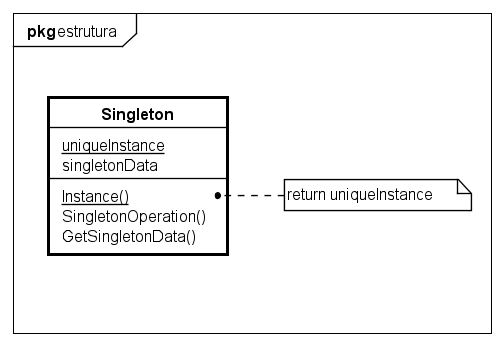
\includegraphics[scale=0.6]{5_padroes-contexto-funcional/5.1_criacionais/5.1.5_singleton/singleton_estrutura.png}
    \end{center}
    \legend{Fonte: \cite{gamma:1995}}
\end{figure}

\subsection*{Participantes}

Descreve as responsabilidades de cada classe que 
participa do padrão. Neste caso, existe 
apenas uma: o próprio Singleton, que define 
a operação de classe Instance, permitindo aos clientes 
acessarem sua única instância. Também pode ser o 
responsável por criar sua própria instância única.

\subsection*{Colaborações}

Este tópico explica como as classes participantes 
colaboram para executar as responsabilidades 
especificadas. Para o Singleton, os clientes (ou seja, 
os objetos que o acessam) acessam a instância única 
pela operação Instance.

\subsection*{Consequências}

As consequências descrevem os custos e benefícios para 
que o padrão possa realizar seu objetivo, além dos 
aspectos da estrtura de um sistema que ele permite variar 
independentemente. O Singleton enumera cinco benefícios:

Primeiro, acesso controlado à instância única, já que 
a única instância é encapsulada dentro da classe 
Singleton, ela possui controle total de como e quando 
ela pode ser acessada pelos clientes.

Segundo, espaço de nomes reduzido. Uma alternativa 
para o Singleton talvez fosse o uso de variáveis 
globais, porém o padrão evita que o espaço de nomes 
seja poluído com variáveis globais que utilizam 
instâncias únicas.

Terceiro, ele permite um refinamento de operações e da 
representação, ou seja, permite ao Singleton ter 
subclasses.

Quarto, permite um número variável de instâncias. Nesse 
caso, o padrão permite que, após ele ser implementado, 
seja simples mudar de ideia e a própria classe Singleton, 
dentro da operação Instance, volte a permitir um número 
indefinido ou até controlado de instâncias.

Quinto, é mais flexível do que operações de classe. Além 
das variáveis globais, operações de classe seriam outra 
alternativa para o Singleton, porém isso tornaria mais 
difícil voltar a ter mais de uma instância da classe, 
além de impedir, em certas linguagens, que subclasses 
redefinam operações estáticas polimorficamente.

\subsection*{Implementação}

Explicita sugestões, técnicas ou riscos que devem 
ser conhecidos durante a implementação do padrão, 
além de considerações específicas de algumas 
linguagens. Para o Singleton, existem duas 
explicações de implementação.

A primeira refere-se à garantia da existência de 
apenas uma instância, onde é sugerido tornar a operação 
de criação do Singleton em uma operação de classe 
que possui acesso a um atributo que armazena a 
instância do Singleton, caso já exista. A segunda 
trata da criação de subclasses da classe Singleton, 
onde é sugerido registrar cada instância por nome 
para que uma classe cliente possa acessar o singleton 
desejado sem precisar conhecer todas as instâncias 
existentes. Ambas as implementações são 
exemplificadas na seção de exemplo de código.


\subsection*{Exemplo de Código}

Como o nome já diz, demonstra o padrão através de 
um exemplo em código. O exemplo do Singleton é um 
construtor de labirintos, onde a classe que é 
responsável pela fabricação dos labirintos necessita 
de apenas uma instância. O código \ref{singletonnosub}
apresenta a implementação do padrão sem o uso de 
subclasses, enquanto o código \ref{singletonsub} 
apresenta uma versão com o uso de subclasses, 
onde as subclasses referenciadas são BombedMazeFactory  
e EnchantedMazeFactory. 
Ambos estão na linguagem C++ e foram retirados 
do livro, porém a implementação pode ser feita 
de forma equivalente em qualquer linguagem 
orientada a objetos.

\begin{lstlisting}[caption={Exemplo de Singleton sem subclasses}, label=singletonnosub]
    
    class MazeFactory {
    public:
        static MazeFactory* Instance();

        // interface existente vai aqui
    protected:
        MazeFactory();
    private:
        static MazeFactory* _instance;
    };


    // implementação:

    MazeFactory* MazeFactory::_instance = 0;

    MazeFactory* MazeFactory::Instance () {
        if (_instance == 0) {
            _instance = new MazeFactory;
        } 
        return _instance;
    } 

\end{lstlisting}
\legend{Fonte: \cite{gamma:1995}}


\begin{lstlisting}[caption={Exemplo de Singleton com subclasses},label=singletonsub]
    
    MazeFactory* MazeFactory::Instance () {
        if (_instance == 0) {
            const char* mazeStyle = getenv("MAZESTYLE");

            if (strcmp(mazeStyle, "bombed") == 0) {
                _instance = new BombedMazeFactory;

            } else if (strcmp(mazeStyle, "enchanted") == 0) {
                _instance = new EnchantedMazeFactory;

            // ... outras subclasses possíveis

            } else { // default
                _instance = new MazeFactory;
            }
        }
        return _instance;
    } 

\end{lstlisting}
\legend{Fonte: \cite{gamma:1995}}


\subsection*{Usos Conhecidos}

Demonstra usos desse padrão em sistemas reais. No caso 
do Singleton, é mencionado o relacionamento entre 
classes e suas metaclasses. Um exemplo atual de uso 
de Singleton é a ferramenta de injeção de dependência 
do .NET Core, onde um serviço 
pode comportar-se como um Singleton\cite{didotnet}.

\subsection*{Padrões Relacionados}

Os padrões relacionados apresentam padrões que 
possuem alguma relação ou que podem ser usados juntos 
do padrão proposto. São mencionados padrões que 
podem ser implementados utilizando o Singleton, que 
são o AbstractFactory, o Builder e o Prototype.



\chapter{Scala}

A maior parte deste trabalho utiliza demonstrações 
e exemplos implementados na linguagem de programação Scala. 
Por ser uma linguagem que mistura os conceitos de 
orientação e objetos e programação funcional, ela traz 
facilidades para transpor os conceitos e os padrões, porém, 
traz uma sintaxe que destoa do que é comumente visto 
em linguagens orientadas a objetos, o que pode prejudicar 
a compreensão dos exemplos em código dos padrões de projeto. 
O objetivo deste capítulo é explicar alguns conceitos e 
sintaxes da linguagem que serão vistos posteriormente.


\section{Construtores}

Em Scala, um construtor pode ser definido como todo o 
bloco de código envolvido pelas chaves na definição da 
classe, o que inclui também a declaração dos métodos 
e dos atributos\cite{wampler2021}. O exemplo mais 
simples de um construtor 
está no código \ref{scalaconstructor1}, onde a classe 
Person define os atributos firstName e lastName, que 
devem ser passados durante a instanciação da classe. 
Apenas essa linha é equivalente ao código \ref{javaconstructor1}, 
implementado em Java.

\begin{lstlisting}[caption={Construtor Simples em Scala},label=scalaconstructor1]

    class Person(var firstName : String, var lastName : String)

\end{lstlisting}


\begin{lstlisting}[caption={Construtor Simples em Java},label=javaconstructor1]

    public class Person {
        
        private string firstName;
        private string lastName;
        
        public Person(String firstName, string lastName){
            this.firstName = firstName;
            this.lastName = lastName;
        }
        
        public String getFirstName(){
            return this.firstName;
        }
        
        public String getLastName(){
            return this.lastName;
        }
        
        public void setFirstName(String firstName){
            this.firstName = firstName;
        }
        
        public void setLastName(String lastName){
            this.lastName = lastName;
        }
    }

\end{lstlisting}

Scala também faz uso de construtores auxiliares, definidos 
através de métodos com o nome this\cite{wampler2021}. 
Dessa forma, é possível 
definir instâncias mais flexíveis para uma classe. Esse 
recurso pode ser visto no código \ref{scalaconstructor2}.

\begin{lstlisting}[caption={Construtor Auxiliar em Scala},label=scalaconstructor2]

    class Person(var firstName : String, var lastName : String) {
       
        def this(firstName : String) {
          this(firstName, "Bar")
        }
    
        def this() {
          this("Foo", "Bar")
        }
      
        def Operation(): Unit = {
          println(lastName + ", " + firstName)
        }
  
    }
  
\end{lstlisting}



\section{Var e Val}

A linguagem também permite definir, através das 
palavras chave var e val, valores 
mutáveis ou imutáveis. Ao declarar um atributo com 
a palavra chave val, o atributo torna-se imutável, 
sendo impossível alterar seu valor.\cite{wampler2021, ordesky2008} 
Definir um atributo 
como val é semelhante a definir uma classe sem um 
método \textit{setter} para aquele atributo. Caso 
o código \ref{scalaconstructor1} seja refatorado 
para tornar o atributo lastName imutável, como no código 
\ref{immutableattr}, a implementação em Java vista no 
código \ref{javaconstructor1} tornaria-se semelhante à do código 
\ref{javaimmutableattr}.

\begin{lstlisting}[caption={Exemplo de Atributo Imutável},label=immutableattr]

    class Person(var firstName : String, var lastName : String)

\end{lstlisting}

\begin{lstlisting}[caption={Construtor Simples em Java},label=javaimmutableattr]

    public class Person {
        
        private string firstName;
        private string lastName;
        
        public Person(String firstName, string lastName){
            this.firstName = firstName;
            this.lastName = lastName;
        }
        
        public String getFirstName(){
            return this.firstName;
        }
        
        public String getLastName(){
            return this.lastName;
        }
        
        public void setFirstName(String firstName){
            this.firstName = firstName;
        }
    }

\end{lstlisting}


\section{Trait}

Uma trait é semelhante a uma interface em qualquer 
linguagem orientada a objetos. Ela define uma abstração 
de um comportamento e pode ser implementada por uma 
classe para indicar que ela implementa esse comportamento.\cite{ordesky2008} 
O código \ref{traitexample} define uma trait IButton com 
o método Click. Qualquer classe que implemente essa trait 
precisará definir uma implementação para o método Click. 
Já o código \ref{traitclassexample} mostra a classe 
Button, que implementa a trait IButton, e define a 
implementação de Click.

\begin{lstlisting}[caption={Exemplo de Trait},label=traitexample]

    trait IButton {
      def Click();
    }

\end{lstlisting}

\begin{lstlisting}[caption={Exemplo de classe que implementa uma trait},label=traitclassexample]

    class Button extends IButton {
      def Click(): Unit = println("Clicked")
    }

\end{lstlisting}

Apesar das semelhanças, diferente das interfaces em 
linguagens como Java, as traits podem definir métodos 
com implementações e até atributos, podendo servir 
como \textit{mixins}\cite{wampler2021}. Isso permite que 
as traits também possam ser usadas como alternativa 
às classes abstratas em casos específicos. Porém, para 
simplificar o entendimento dos exemplos deste 
trabalho por parte de leitores não familiarizados 
com a linguagem Scala, as traits serão utilizadas 
apenas como alternativa às interfaces.


\section{Operadores e Atributos de Classe}

A linguagem Scala não possui o modificador \textit{static}, 
utilizado para definir atributos e métodos de classe - 
ou seja, atributos e métodos que existem independentes 
da instância de uma classe. 

Isso pode ser contornado através de \textit{companion objects}. 
Um exemplo pode ser visto no código \ref{coexample}, onde 
existe a classe Companion e seu \textit{companion object}, que 
deve possuir o mesmo nome e ser definido no mesmo arquivo 
que a classe. A operação StaticOperation é executada 
independente de existir uma instância da classe, acessada 
apenas através do nome Companion.

Externamente, os \textit{companion objects} são acessados 
de forma semelhante aos membros estáticos de uma classe 
em Java, por exemplo. Isso pode ser visto no código 
\ref{coexample2}, onde o método StaticOperation é acessado 
na função principal de um programa.

\begin{lstlisting}[caption={Exemplo de companion object},label=coexample]

class Companion(private var name : String) {
  def ClassOperation(): Unit = {
    Companion.StaticOperation(name)
  }
}

object Companion {
  def StaticOperation(name : String): Unit = {
    println("Hello, " + name)
  }
}

\end{lstlisting}

\begin{lstlisting}[caption={Chamada de operações de um companion object},label=coexample2]

object Main {
  def main(args : Array[String]) : Unit = {
    Companion.StaticOperation("Name1")
    var companion = new Companion("Name2")
    companion.ClassOperation()
  }
}

\end{lstlisting}

\section{Listas imutáveis}

Diferente das coleções vistas comumente em linguagens 
orientadas a objeto, em Scala as listas são tipos 
imutáveis. Isso significa que uma operação de adição 
ou concatenação em uma lista não modificará a lista 
que realiza a operação, mas sim retornará uma nova 
lista\cite{ordesky2008}. 

Os códigos \ref{listadd} e \ref{listconcat} demonstram 
as operações de adição e concatenação em uma lista, 
respectivamente. É importante ressaltar que, mesmo 
as listas sendo imutáveis, o fato do 
atributo numbers ter sido declarado como var 
faz com que ele possa ser reatribuído com a nova lista 
resultante da operação.

\begin{lstlisting}[caption={Exemplo de adição em uma lista imutável},label=listadd]

  var numbers : List[Int] = List()
  
  def AddElement(number : Int): Unit ={
    numbers = number :: numbers
  }

\end{lstlisting}

\begin{lstlisting}[caption={Exemplo de concatenação em uma lista imutável},label=listconcat]

  var numbers : List[Int] = List()
  
  def ConcatElements(newNumbers : List[Int]): Unit = {
    numbers = newNumbers ::: numbers
  }    

\end{lstlisting}

\section{Unit}

Em diversos exemplos em código desse capítulo 
(linha 12 em \ref{scalaconstructor2}, linha 3 em 
\ref{traitclassexample}, linha 4 em 
\ref{listadd} e linha 4 em \ref{listconcat}) 
foi possível ver a palavra chave Unit. Ela é semelhante ao 
valor void utilizado em linguagens de programação como C e 
Java para indicar que uma função ou método não retorna 
nenhum valor\cite{wampler2021}.




% ----------------------------------------------------------
% PARTE
% ----------------------------------------------------------
\part{Desenvolvimento}
% ----------------------------------------------------------


% ---
% Capitulo de revisão de literatura
% ---
\chapter{Orientação a Objetos no Contexto Funcional}
% ---

% Conceitos para mapear

Parte dos padrões de projeto que serão 
analisados dependem de conceitos 
de orientação a objetos como classes ou 
encapsulamento, o que torna necessário 
realizar um mapeamento desses conceitos 
para o paradigma funcional. A intenção 
desse mapeamento não é implementar 
orientação a objetos em uma linguagem 
funcional, mas entender qual é a utilidade 
de cada um desses conceitos e de que 
forma a programação funcional pode 
oferecer essa mesma utilidade. É importante 
ressaltar que esse mapeamento não será usado 
de forma metódica ao analisar os padrões. 
Ele é uma referência para contextualizar 
o leitor nos exemplos em código 
implementados de forma funcional. 


% classes e objetos
\section{Classes e Objetos}

Um objeto pode ser definido como uma representação 
do mundo real que possui características e comportamentos, 
enquanto uma classe é uma abstração dessa representação 
que define quais características e comportamentos um objeto 
deve possuir\cite{umlsystems}. Essas características 
e comportamentos são representados em orientação a 
objetos como atributos e métodos, respectivamente. 
O Código \ref{ooclass} demonstra uma classe que 
possui os atributos \texttt{nome} e \texttt{idade}, além dos métodos 
\texttt{getNome}, \texttt{setNome}, \texttt{getIdade} 
e \texttt{setIdade}, que realizam 
operações com esses atributos.

\begin{lstlisting}[caption={Exemplo de classe em Orientação a Objetos.},label=ooclass]
    
    class Pessoa(var nome : String, var idade : Int){

        def getNome() : String = this.nome

        def setNome(nome : String) : Unit = this.nome = nome

        def getIdade() : Int = this.idade

        def setIdade(idade : Int) : Unit = this.idade = idade

    }   

\end{lstlisting}

Dessa forma, é necessário definir uma estrutura em 
programação funcional que possua características e 
funções que operam sobre essas características. 
Para agrupar características pode ser utilizada uma 
tupla, uma estrutura que armazena uma quantidade 
fixa de valores com tipos predefinidos\cite{tuplesscala}. 
Como as tuplas não podem ser modificadas, elas 
respeitam o conceito de imutabilidade das 
linguagens funcionais.

Para representar os métodos de uma classe em uma 
linguagem funcional, já que nossa estrutura de dados 
imutável não armazenará funções\footnote{Apesar de não 
ser uma abordagem utilizada para este mapeamento, é 
possível armazenar funções em tuplas.} e já 
que é necessário que nossas funções sejam puras, 
uma abordagem de implementação desses 
métodos é definir funções que recebam 
como parâmetro um valor do tipo definido em nossa 
estrutura de dados imutável. Seguindo esses dois 
princípios, uma versão funcional da classe apresentada 
no Código \ref{ooclass} pode ser vista no Código \ref{fpclass}
\footnote{ 
Este exemplo possui as notações \textit{\textunderscore1} e 
\textit{\textunderscore2}, 
que são a forma que a 
linguagem Scala utiliza para acessar a primeira e 
a segunda posição de uma tupla, respectivamente.
}.



\begin{comment}
    \footnote{
    O Código \ref{fpclass} possui as notações 
    pessoa._1 e pessoa._2, que são a forma que a 
    linguagem Scala utiliza para acessar a primeira e 
    a segunda posição de uma tupla, respectivamente.
}
    possui as notações 
\textit{._1} e \textit{._2}, que são a forma que a 
linguagem Scala utiliza para acessar a primeira e 
a segunda posição de uma tupla, respectivamente
\end{comment}

\begin{lstlisting}[caption={Representação de uma classe no contexto funcional.},label=fpclass]
    
    type Pessoa = (String, Int)

    def getNome(pessoa : Pessoa) : String = pessoa._1 

    def setNome(pessoa : Pessoa, name : String) : Pessoa = 
        (name, pessoa._2)

    def getIdade(pessoa : Pessoa) : Int = pessoa._2

    def setIdade(pessoa : Pessoa, age : Int) : Pessoa =
        (pessoa._1, age)

\end{lstlisting}

%associação
\section{Associação, Agregação e Composição}

Uma associação pode ser definida como uma 
conexão entre as classes que indica algum 
relacionamento entre elas\cite{Sommerville10}. 
O código \ref{ooassociation} demonstra uma 
associação entre as classes Cidade e Estado, onde 
a classe Estado possui uma coleção de atributos 
do tipo Cidade. Para que haja uma associação 
entre duas classes, basta que pelo menos 
uma delas tenha em seus atributos uma 
referência à outra.

\begin{lstlisting}[caption={Exemplo de associação entre classes.},label=ooassociation]
    
    class Cidade(var nome : String){

        def getNome() : String = this.nome;
        def setNome(nome : String) : Unit {
            this.nome = nome;
        }
    }

    class Estado(var nome : String, var cidades : List[Cidade]){

        def getNome() : String = this.nome;
        def setNome(nome : String) : Unit {
            this.nome = nome;
        }
        def getCidades() : List[Cidade] = this.cidades;
        def addCidade(cidade : Cidade) : Unit {
            this.cidades = this.cidades :+ cidade;
        }
    }

\end{lstlisting}

Como foi visto anteriormente, os atributos 
podem ser representados por valores salvos 
dentro de uma tupla associada a um tipo. 
Portanto, uma associação dentro do contexto 
funcional pode ser implementada armazenando 
um valor de um tipo A entre os valores da tupla 
de um tipo B. O Código \ref{fpassociation} 
demonstra o exemplo anterior implementado 
de forma funcional.

\begin{lstlisting}[caption={Exemplo de associação no contexto funcional.},label=fpassociation]
    
    type Cidade = (String)
    
    def getNome(cidade : Cidade) : String = cidade._1;
    def setNome(cidade : Cidade, nome : String) : Cidade = (nome)

    type Estado = (String, List[Cidade])
    
    def getNome(estado : Estado) : String = estado._1;
    def setNome(estado : Estado, nome : String) : Estado = (nome, estado._2)
    
    def getCities(estado : Estado) : List[Cidade] = estado._2;
    def addCity(estado : Estado, cidade : Cidade) : Estado =
        (estado._1, estado._2 :+ cidade)

\end{lstlisting}

% encapsulamento
\section{Encapsulamento}

A abordagem da seção anterior implementa 
classes e objetos, porém precisa ser 
reavaliada para que possa levar em consideração 
o encapsulamento. Encapsulamento pode ser definido 
como uma forma de limitar o acesso a um conjunto 
de dados ou comportamentos de um objeto \cite{quarkoo}. 
A motivação para isso pode vir tanto da necessidade 
de concentrar as alterações externas que um objeto 
pode sofrer em apenas um lugar quanto evitar que 
esse objeto assuma um estado que não deveria ser 
representado. 

Com a ideia de imutabilidade, pode-se 
assumir que um valor não será alterado em partes 
diferentes de uma aplicação, mas é possível 
que funções responsáveis por criar ou modificar\footnote{
    Uma função que modifica um valor é entendida 
    como uma função que recebe um valor existente 
    por parâmetro e retorna um novo valor do mesmo 
    tipo.
} 
um valor de um determinado tipo estejam 
espalhadas pela aplicação, facilitando uma 
situação em que um estado que não deveria ser 
representado por esse valor seja criado. 
Dessa forma, implementar alguma forma de 
encapsulamento ainda é importante no 
contexto funcional.

Existe mais de uma abordagem que torna 
possível implementar o encapsulamento em 
linguagens funcionais, o uso de GADTs - 
\textit{Generalized Algebraic 
Data Types}\cite{existentialhaskell} - é uma 
delas. \textit{Closures} também podem 
ser utilizadas ao armazenar valores de 
atributos enquanto retorna as funções 
necessárias para acessá-los ou modificá-los. 
Um exemplo equivalente ao do Código \ref{fpclass} 
pode ser visto no Código \ref{fpclosure}, 
implementado utilizando a linguagem funcional Clojure. 
\cite{classlessjs} Nele, a função pessoa 
funciona como um construtor que recebe como 
parâmetro o nome e a idade de uma pessoa e 
retorna um dicionário com as funções para 
recuperar ou modificar o estado de uma pessoa.
As funções de modificação retornam uma nova versão 
da pessoa com o estado alterado.

\begin{lstlisting}[caption={Representação de uma classe com \textit{closures}.},label=fpclosure]
    
    (defn pessoa [nome idade]
        {:getNome nome
         :setNome (fn [_nome] (pessoa _nome idade))
         :getIdade idade
         :setIdade (fn [_idade] (pessoa nome _idade))})

\end{lstlisting}

Apesar de não ser um conceito de programação 
funcional, também é possível aproveitar a ideia 
de modularização para esconder detalhes de 
implementação \cite{mlmodules}. Por exemplo, o 
Código \ref{modulesencap}, implementado em 
Haskell
\footnote{
    Como a linguagem Scala utiliza palavras-chave 
    como \textit{object} e \textit{private} para 
    implementar módulos, o exemplo foi feito em 
    Haskell para que não fosse associável à 
    orientação a objetos.
}
, mostra o tipo \texttt{Pessoa} com um construtor 
\texttt{P}. Apesar do tipo \texttt{Pessoa} ser exportado para fora do 
módulo, \texttt{P} não é, tornando impossível para qualquer 
função que acesse esse módulo criar algo do tipo 
\texttt{Pessoa}. Dessa forma, apenas a função \texttt{newPessoa}, 
também exportada pelo módulo, 
pode criar novos valores do tipo 
\texttt{Pessoa}. Funções implementadas dentro do módulo 
também podem deixar de ser exportadas, o que 
as tornaria semelhantes a métodos privados 
de uma classe.

\begin{lstlisting}[caption={Módulos como forma de encapsulamento.},label=modulesencap]
    
    module Pessoa (Pessoa, newPessoa, getNome, setNome, getIdade, setIdade) where

    data Pessoa = P (String, Int)

    newPessoa :: String -> Int -> Pessoa
    newPessoa nome idade = P (nome, idade)

    getNome :: Pessoa -> String
    getNome (P (nome, _)) = nome

    setNome :: Pessoa -> String -> Pessoa
    setNome (P (_, idade)) nome = P (nome, idade)

    getIdade :: Pessoa -> Int
    getIdade (P (_, idade)) = idade

    setIdade :: Pessoa -> Int -> Pessoa
    setIdade (P (nome, _)) idade = P (nome, idade)

\end{lstlisting}

Todas essas abordagens são válidas para a 
implementação do encapsulamento, sendo a 
linguagem utilizada um fator mais decisivo 
do que a abordagem em si. Por exemplo, é 
mais simples implementar a abordagem de \textit{closures} 
em Clojure por ela ser dinamicamente tipada, 
permitindo que um dicionário sem estrutura 
predefinida seja retornado. Linguagens que exigem 
uma definição mais estrita do tipo de retorno 
de uma função podem dificultar tanto a 
implementação dessas funções quanto seu uso 
no resto do programa.

Sendo o objetivo dessa seção demonstrar que 
o encapsulamento pode ser implementado e 
não definir como implementá-lo, 
a abordagem utilizada para o encapsulamento 
durante a análise dos padrões será 
omitida, a menos que ela seja relevante para 
sua implementação. Essa omissão 
também tem como objetivo não particularizar o 
método de encapsulamento utilizado durante a 
implementação dos exemplos.

% interfaces
\section{Interfaces}

Uma interface pode ser entendida como um contrato 
entre uma classe e o mundo externo, indicando que 
uma classe que implementa uma interface também 
implementará as operações definidas 
pela mesma\cite{oracleooconcepts}. 

Um exemplo do uso de interfaces é demonstrado no Código 
\ref{oopinterface1}, 
onde a interface é necessária para garantir que as 
classes \texttt{SomadorMaisUm} e \texttt{MultiplicadorPorDois} 
implementem 
a operação \texttt{calcular}, que recebe como parâmetro 
um valor do tipo inteiro e retorna outro valor 
inteiro.

% Exemplo 1 de Interfaces

\begin{lstlisting}[caption={Interfaces em Orientação a Objetos.},label=oopinterface1]
    
    trait ICalculaInteiro {
        def calcular(x : Int) : Int
    }

    class SomadorMaisUm extends ICalculaInteiro {
        def calcular(x : Int) : Int = x + 1
    }

    class MultiplicadorPorDois extends ICalculaInteiro {
        def calcular(x : Int) : Int = 2*x
    }

    def calcularInteiro(x : Int, calculador : ICalculaInteiro) : Int {
        return calculador.calcular(x)
    }

\end{lstlisting}

Utilizando funções de alta ordem e levando em 
consideração que as funções que representam nossos 
métodos não estão encapsulados em classes e 
não dependem de atributos, é possível substituir o 
objeto sendo passado por parâmetro na função 
\texttt{calcularInteiro} por uma função qualquer que recebe 
como parâmetro um valor inteiro e retorna outro 
valor inteiro. Essa alternativa pode ser vista 
no Código \ref{fpinterface1}.

\begin{lstlisting}[caption={Interfaces em Programação Funcional.},label=fpinterface1]
    
    def somaUm(x : Int) : Int = x + 1

    def multiplicaPorDois(x : Int) : Int = 2*x

    def calcularInteiro(x : Int, calcular : (Int => Int)) =
        calcular(x)
    
\end{lstlisting}



% herança
\section{Herança}

Quando é desejado que uma classe seja incluída ou 
utilizada como base para a criação de outra classe, 
usa-se a herança\cite{quarkoo}. Dessa forma, é 
possível criar implementações mais específicas 
de classes já existentes e reaproveitar o código. 
O Código \ref{ooinheritance} demonstra 
o uso da herança entre as classes \texttt{Animal} 
e \texttt{Cachorro}. 
Ao invés de reimplementar os métodos da classe 
\texttt{Animal}, a classe \texttt{Cachorro} usa herança 
para reaproveitá-los. 

\begin{lstlisting}[caption={Herança em Orientação a Objetos.},label=ooinheritance]
    
    class Animal(var nome : String) {
        def getNome() : String = nome
        
        def comer() : String {
            return "Meu nome é " + nome + " e eu posso comer";
        }
    }

    class Cachorro extends Animal {
        
        def Cachorro(nome : String) {
            super(nome);
        }

        def latir() : String {
            return "Au! Meu nome é " + super.getNome();
        }

        def comer() : String {
            return super.comer() + "\nEu como comida de cachorro";
        }
    }

\end{lstlisting}

No contexto funcional, um comportamento semelhante 
pode ser alcançado através da composição. Um tipo A 
que deseja herdar as funcionalidades de um tipo B 
deve possuir uma instância desse mesmo tipo em seus 
atributos. Para os métodos do tipo A, basta que as 
funções do tipo B sejam compostas das funções 
necessárias do tipo A. O Código \ref{fpinheritance} 
demonstra o exemplo anterior, onde um tipo \texttt{Animal} 
armazena um valor \textit{string} que representa o nome 
enquanto o tipo \texttt{Cachorro} armazena um valor \texttt{Animal}. 
As funções \texttt{latir} e \texttt{comer} que recebem como parâmetro 
um valor do tipo \texttt{Cachorro} reutilizam as funções \texttt{getNome} 
e \texttt{comer} que recebem como parâmetro um valor do tipo 
\texttt{Animal}. Nesse exemplo, o tipo \texttt{Animal} representa 
uma classe pai e o tipo \texttt{Cachorro} uma classe filha.

\begin{lstlisting}[caption={Herança em Programação Funcional},label=fpinheritance]
    
    type Animal = (String)

    def getNome(animal : Animal) : String = animal._1;
    def comer(animal : Animal) : String = 
        "Meu nome é " + getNome(animal) + " e eu posso comer"

    type Cachorro = (Animal)

    def getAnimal(cachorro : Cachorro) : Animal = cachorro._1;
    def latir(cachorro : Cachorro) : String = 
        "Au! Meu nome é " + getNome(getAnimal(cachorro))
    def comer(cachorro : Cachorro) : String = 
        comer(getAnimal(Cachorro)) + "\nEu como comida de cachorro";

\end{lstlisting}

É possível perceber que a implementação da herança 
assemelha-se à implementação de uma associação, 
por isso ela apresenta uma desvantagem: 
qualquer função do tipo que representa 
a classe pai necessitará de uma função 
intermediária do tipo que representa a classe 
filha para acessá-la. 
No contexto orientado a objetos, esses dois 
relacionamentos são diferentes, pois a 
herança trata-se de um relacionamento entre 
classes enquanto a associação é um relacionamento 
entre objetos\cite{umlsystems}. 


% ----------------------------------------------------------
% CRIACIONAIS
% ----------------------------------------------------------
%\chapter{Padrões Criacionais}

\chapter{Padrões Criacionais}

\section{Factory Method}

O padrão Factory Method tem como objetivo oferecer, através de uma 
classe Factory, uma interface para a criação de objetos. Esses objetos, 
porém, podem ser configurados através de classes que herdam de Factory.


\begin{figure}[htb]
	\caption{\label{fig_grafico}Estrutura do Factory Method}
	\begin{center}
	    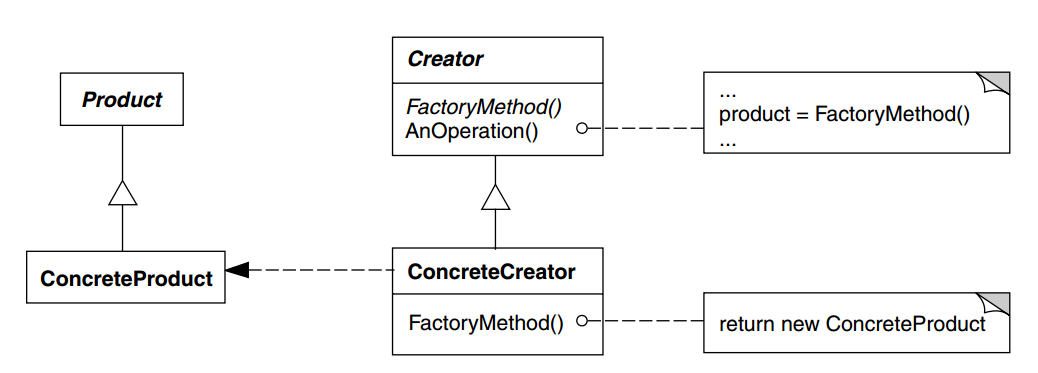
\includegraphics[scale=0.5]{5_padroes-contexto-funcional/5.1_criacionais/5.1.1_factory-method/diagram.png}
	\end{center}
\end{figure}

Exemplo Orientado a Objetos:

\begin{lstlisting}[caption={Factory Method Orientado a Objetos},label=oofactory]
    
    trait Product{
        def doStuff() : Unit
    }

    class ConcreteProduct extends Product(){

        def doStuff() : Unit = {
            
        }
    }

    abstract class Creator(){

        def someOperation() : Unit = {
            var p = createProduct()
            p.doStuff()
        }

        def createProduct() : Product
    }

    class ConcreteCreator() extends Creator{

        def createProduct() : Product = {
            return new ConcreteProduct()
        }
    }

\end{lstlisting}

Contexto Funcional:

\begin{lstlisting}[caption={Factory Method Funcional},label=fpfactory]
    
    

\end{lstlisting}
\section{Abstract Factory}

O padrão \textit{Abstract Factory} define uma família 
de objetos relacionados e uma interface para 
criá-los, sem definir sua implementação. Dessa 
forma, diferentes implementações desse 
conjunto de objetos podem ser utilizadas 
sem que as classes cliente que os utilizam 
precisem conhecê-las.\cite{gamma:1995}

O diagrama apresentado na Figura \ref{abfactory_struct} 
demonstra a estrutura desse padrão, onde a 
interface \texttt{AbstractFactory} suporta as famílias 
\texttt{ConcreteFactory1} e \texttt{ConcreteFactory2}, com cada uma 
delas definindo qual implementação das interfaces 
\texttt{AbstractProductA} e \texttt{AbstractProductB} serão 
utilizadas.

\begin{figure}[htb]
	\caption{\label{abfactory_struct}Estrutura do \textit{Abstract Factory}.}
	\begin{center}
	    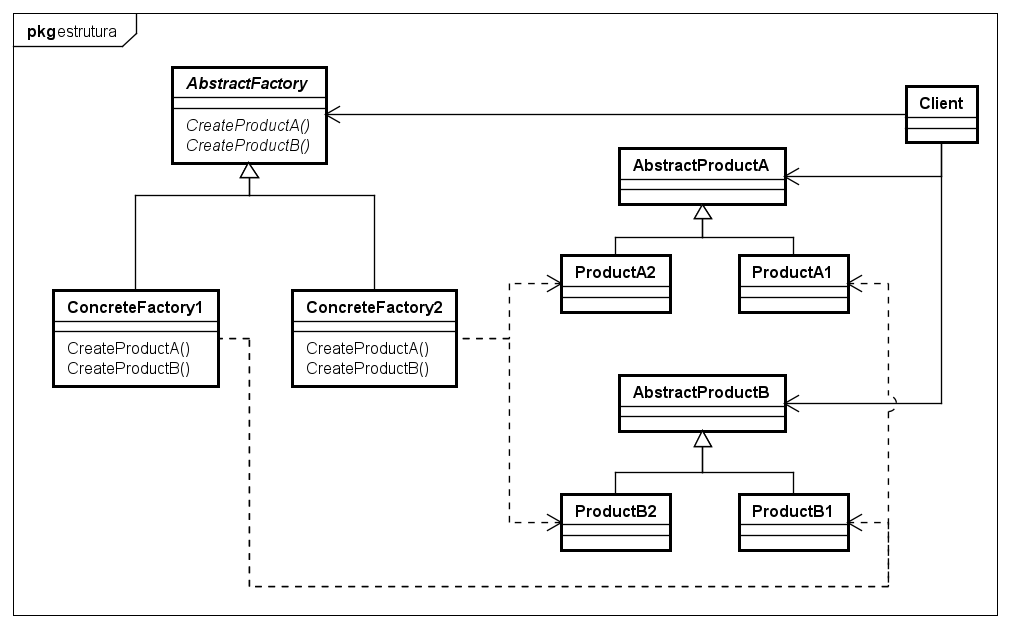
\includegraphics[scale=0.5]{5_padroes-contexto-funcional/5.1_criacionais/5.1.2_abstract-factory/abstractfactory_estrutura.png}
	\end{center}
  \caption*{Fonte: O Autor (2021)}
\end{figure}

\subsection*{Exemplo Orientado a Objetos}

Como exemplo, é apresentado um \textit{toolkit} 
que suporta tipos diferentes de interação para 
seus \textit{widgets}, como \textit{Motif} ou \textit{Presentation 
Manager} (PM). Dessa forma, para que o \textit{toolkit} 
não precise ser implementado tendo conhecimento 
de cada tipo diferente de \textit{widget}, é 
utilizado o padrão \textit{Abstract Factory} para 
definir uma família de objetos de \textit{widget} 
diferente para cada tipo de interação. 

A implementação do padrão é demonstrada no 
diagrama de classes da Figura \ref{abfactory_exemplo} 
e no Código \ref{ooabfactory}. Uma interface 
\texttt{WidgetFactory} define as operações de criação 
de todos os \textit{widgets} possíveis, enquanto 
as classes \texttt{MotifWidgetFactory} e \texttt{PMWidgetFactory} 
implementam sua criação para os tipos de 
interação suportados.

\begin{figure}[htb]
	\caption{\label{abfactory_exemplo}Exemplo de \textit{Abstract Factory}.}
	\begin{center}
	    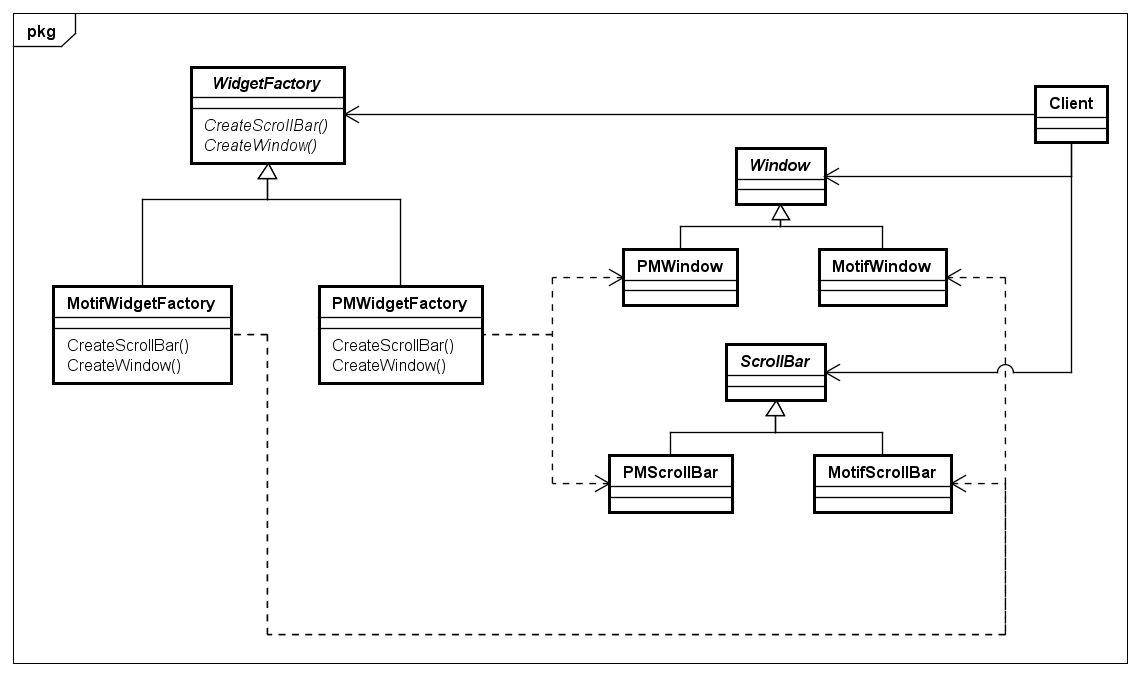
\includegraphics[scale=0.5]{5_padroes-contexto-funcional/5.1_criacionais/5.1.2_abstract-factory/abstractfactory_exemplo.png}
	\end{center}
  \caption*{Fonte: O Autor (2021)}
\end{figure}

\begin{lstlisting}[caption={\textit{Abstract Factory} Orientado a Objetos.},label=ooabfactory]
	
trait WidgetFactory {
  def CreateScrollBar() : ScrollBar
  def CreateWindow() : Window
}

trait Window 
trait ScrollBar

class MotifWidgetFactory extends WidgetFactory {
  def CreateScrollBar(): ScrollBar = new MotifScrollBar()
  def CreateWindow(): Window = new MotifWindow()
}

class PMWidgetFactory extends WidgetFactory {
  def CreateWindow(): Window = new PMWindow()
  def CreateScrollBar(): ScrollBar = new PMScrollBar()
}

class PMWindow extends Window {
  // Implementação de PMWindow
}

class MotifWindow extends Window {
  // Implementação de MotifWindow
}

class PMScrollBar extends ScrollBar {
  // Implementação de PMScrollBar
}

class MotifScrollBar extends ScrollBar {
  // Implementação de MotifScrollBar
}

\end{lstlisting}
\legend{Fonte: O Autor (2021)}


\subsection*{Contexto Funcional}

As classes e interfaces \textit{factory} podem 
ser substituídas por funções de alta ordem 
recebidas pela função cliente. 
No Código \ref{fpabfactory} são definidos, 
nas linhas 2 e 3,  
os tipos \texttt{ScrollBar} e \texttt{Window} referentes aos 
\textit{widgets} suportados pela ferramenta. 
Da mesma forma, são definidas as operações de 
criação desses \textit{widgets} para os tipos 
\texttt{PM} e \texttt{Motif}. Nas linhas 5 e 8 são definidas as 
operações para o tipo \texttt{PM}, enquanto nas linhas 
12 e 15 são definidas as para o tipo \texttt{Motif}. 

Na linha 19 é definida uma função cliente, 
que seria equivalente a uma operação da classe 
\texttt{Client} apresentada no diagrama da Figura 
\ref{abfactory_exemplo}. Ela 
recebe como parâmetro as funções para criação de 
cada \textit{widget}. Por fim, na linha 28 é 
demonstrada a chamada dessa função recebendo 
como parâmetro as funções para criar um 
\textit{scrollbar} e uma janela para o tipo 
\texttt{PM}.

\begin{lstlisting}[caption={\textit{Abstract Factory} Funcional.},label=fpabfactory]
    
type Scrollbar
type Window

def CreatePMScrollBar() : Scrollbar = {
  // Criação da scrollbar PM
}
def CreatePMWindow() : Window = {
  // Criação da janela PM
}

def CreateMotifScrollBar() : Scrollbar = {
  // Criação da scrollbar Motif
}
def CreateMotifWindow() : Window = {
  // Criação da janela Motif
}

def ClientFunction(
  scrollBarFactory : () => Scrollbar, 
  windowFactory : () => Window): Unit = {
  // ...
  val scrollbar = scrollBarFactory()
  val window = windowFactory()
  // ...
}

ClientFunction(CreatePMScrollBar, CreatePMWindow)

\end{lstlisting}
\legend{Fonte: O Autor (2021)}

No Código \ref{fpabfactory}, seria possível passar 
para a classe cliente \textit{widgets} de tipos 
misturados, já que são definidos parâmetros 
diferentes para cada função de criação. Caso 
seja desejado um exemplo mais próximo do demonstrado 
no diagrama da Figura \ref{abfactory_exemplo}, 
pode-se encapsular as funções de criação 
em uma tupla. Isso pode ser visto no Código 
\ref{fpabfactory2}, onde o tipo \texttt{WidgetFactory} 
definido na linha 2 armazena tanto uma função 
para a criação de um \textit{scrollbar} quanto a função 
para a criação de uma janela. A função 
cliente, redefinida na linha 10, agora 
recebe como parâmetro um valor do tipo 
\texttt{WidgetFactory}.

\begin{lstlisting}[caption={\textit{Abstract Factory} Funcional usando tuplas.},label=fpabfactory2]
    
type WidgetFactory = (
  () => ScrollBar, 
  () => Window
)

val PMWidgetFactory : WidgetFactory = 
  (CreatePMScrollBar, CreatePMWindow)

def ClientFunction(factory : WidgetFactory) : Unit = // ...

ClientFunction(PMWidgetFactory)

\end{lstlisting}
\legend{Fonte: O Autor (2021)}
\section{Builder}

Quando é necessário criar objetos  
complexos, o padrão Builder retira a 
responsabilidade de criação do objeto a 
ser criado e a coloca em classes separadas, 
que constroem partes do objeto. 
Isso permite que um mesmo processo de criação 
possa gerar representações diferentes de um mesmo 
objeto.

A figura \ref{builder_struct} apresenta 
a estrutura do Builder, onde a interface 
Builder define uma operação para criar uma 
parte do objeto. A classe ConcreteBuilder, que 
implementa a interface Builder, 
implementa os métodos de construção de 
uma parte do tipo Product. A classe Director 
é responsável por executar a criação das 
partes do objeto, através da operação 
Construct.

\begin{figure}[htb]
	\caption{\label{builder_struct}Estrutura do Builder}
	\begin{center}
	    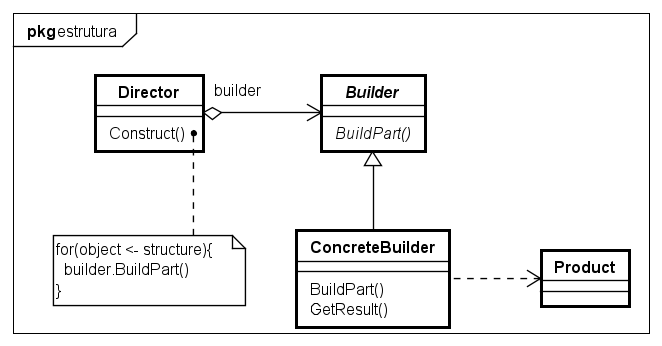
\includegraphics[scale=0.5]{5_padroes-contexto-funcional/5.1_criacionais/5.1.3_builder/builder_estrutura.png}
	\end{center}
\end{figure}

\subsection*{Exemplo Orientado a Objetos}

Como exemplo, podemos observar um leitor de 
documentos do tipo RTF (\textit{Rich Text Format}), 
que deve permitir a conversão de documentos RTF 
para outros formatos, como texto em ASCII ou em um 
\textit{widget} de texto que pode ser editado de 
forma interativa. Como a quantidade de formatos 
possíveis é grande, deve ser possível adicionar 
novos formatos sem que seja necessário modificar 
a classe do leitor de documentos RTF. 

O diagrama de classes apresentado na imagem 
\ref{builder_exemplo} demonstra o uso do padrão 
Builder para esse exemplo. Para cada formato possível 
de conversão, uma nova classe Builder é criada. 
As classes ASCIIConverter, TeXConverter e 
TextWidgetConverter representam, respectivamente, 
os \textit{builders} para os conversores para texto 
em ASCII, LaTeX e \textit{widget} de texto interativo. 
A classe RTFReader chama as operações de construção 
dos conversores desejados. O exemplo de 
implementação dessa abordagem é apresentado no 
código \ref{oobuilder}.

\begin{figure}[htb]
	\caption{\label{builder_exemplo}Exemplo de Builder}
	\begin{center}
	    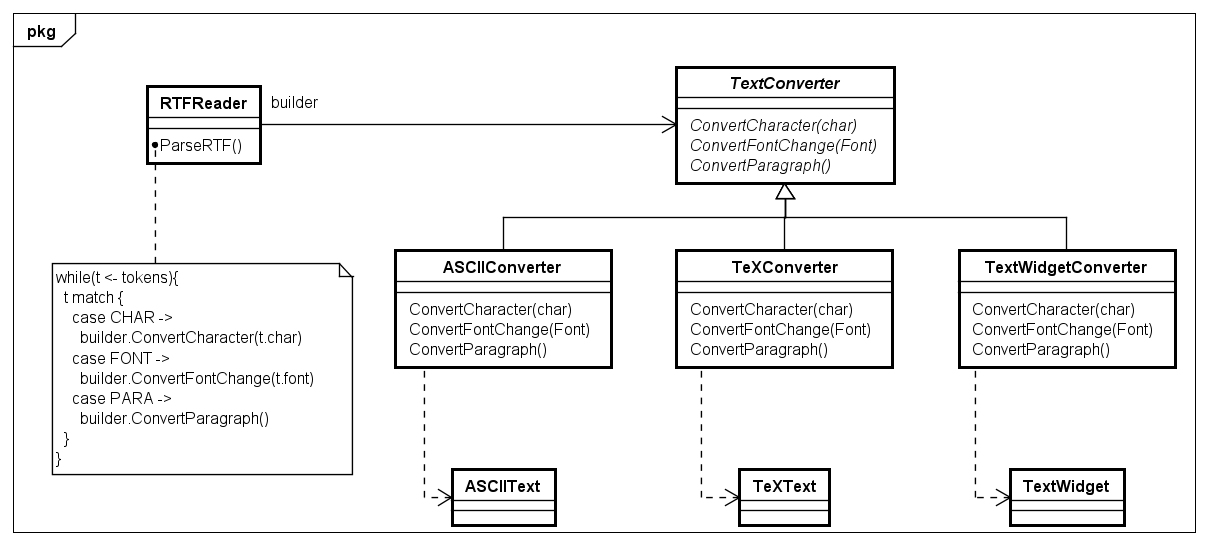
\includegraphics[scale=0.5]{5_padroes-contexto-funcional/5.1_criacionais/5.1.3_builder/builder_exemplo.png}
	\end{center}
\end{figure}

\begin{lstlisting}[caption={Builder Orientado a Objetos},label=oobuilder]

trait TextConverter {
  def ConvertCharacter(char : Char)
  def ConvertFontChange(font : String)
  def ConvertParagraph()
} 

class ASCIIConverter(val asciiText: ASCIIText) extends TextConverter {

  def ConvertCharacter(char : Char): Unit = {
    //Converter char
  }

  def ConvertFontChange(font : String): Unit = {
    //Converter fonte
  }

  def ConvertParagraph(): Unit = {
    //Converte parágrafo
  }
}

class TeXConverter(val texText : TeXText) extends TextConverter {
  def ConvertCharacter(char: Char): Unit = {
    //Converter char
  }

  def ConvertFontChange(font : String): Unit = {
    //Converter fonte
  }

  def ConvertParagraph(): Unit = {
    //Converte parágrafo
  }
}

class TextWidgetConverter(val textWidget: TextWidget) extends TextConverter {
  def ConvertCharacter(char: Char): Unit = {
    //Converter char
  }

  def ConvertFontChange(font : String): Unit = {
    //Converter fonte
  }

  def ConvertParagraph(): Unit = {
    //Converte parágrafo
  }
}

class RTFReader(var textConverter: TextConverter) {

  def SetTextConverter(textConverter: TextConverter): Unit = {
    this.textConverter = textConverter
  }

  def ParseRTF(): Unit = {
    val tokens : List[Token] = List()
    // ...
    for(t <- tokens) {
      t.Type match {
        case TokenType.CHAR => textConverter.ConvertCharacter(t.Character)
        case TokenType.FONT => textConverter.ConvertFontChange(t.Font)
        case TokenType.PARAGRAPH => textConverter.ConvertParagraph()
      }
    }
    // ...
  }
}

\end{lstlisting}

\subsection*{Contexto Funcional}

É possível aproveitar as funções de alta ordem 
da programação funcional para simplificar o 
padrão Builder. Ao invés de definir novas 
classes para cada tipo de builder, uma função 
pode receber como 
parâmetro as operações de construção desejadas. 
No código \ref{fpbuilder}, essa função é a 
ParseRTFBuilder, definida na linha 2. 
Para facilitar o reuso de tipos diferentes 
de \textit{builder}, ela retorna uma nova 
função que recebe como parâmetro uma 
lista de \textit{tokens} e 
retorna uma nova lista no formato desejado. 

A função retornada é análoga ao método 
ParseRTF da classe RTFReader do exemplo 
orientado a objetos. Com essa implementação, 
para cada variação de \textit{builder}, 
basta executar a função 
ParseRTFBuilder passando as operações 
desejadas. Isso pode ser visto na linha 16, 
onde o valor ParseRTFToASCII é o resultado 
da definição do \textit{builder} que converte 
RTF em texto no formato ASCII.

\begin{lstlisting}[caption={Builder Funcional},label=fpbuilder]
    
def ParseRTFBuilder(convertCharacter : Char => Token,
             convertFontChange : String => Token,
             convertParagraph : String => Token)
: List[Token] => List[Token] = (tokens : List[Token]) => {
  val parseRest = (tokens : List[Token]) => ParseRTFBuilder(convertCharacter, convertFontChange, convertParagraph)(tokens)
  // ...
  tokens.head.Type match {
    case TokenType.CHAR => convertCharacter(tokens.head.Character) :: parseRest(tokens.tail)
    case TokenType.FONT => convertFontChange(tokens.head.Font) :: parseRest(tokens.tail)
    case TokenType.PARAGRAPH => convertParagraph(tokens.head.Paragraph) :: parseRest(tokens.tail)
  }
  // ...
}

val ParseRTFToASCII = ParseRTFBuilder(
              ConvertASCIICharacter,
              ConvertASCIIFontChange,
              ConvertASCIIParagraph)
    
\end{lstlisting}
\subsection{Prototype}

\begin{figure}[htb]
	\caption{\label{fig_grafico}Estrutura do Prototype}
	\begin{center}
	    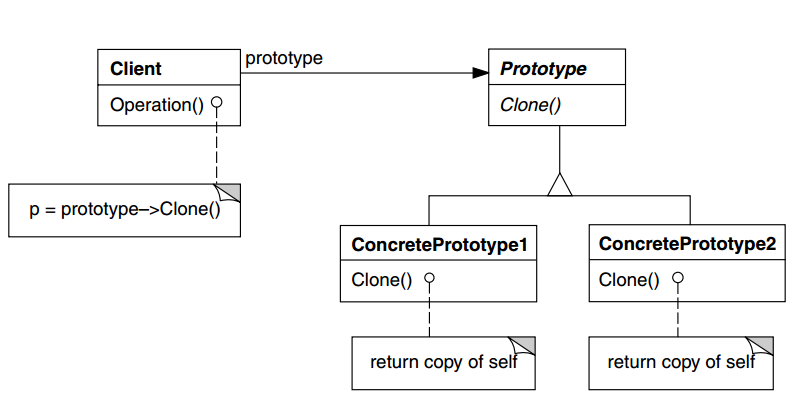
\includegraphics[scale=0.5]{5_padroes-contexto-funcional/5.1_criacionais/5.1.4_prototype/diagram.png}
	\end{center}
\end{figure}

Exemplo Orientado a Objetos:

\begin{lstlisting}[caption={Prototype Orientado a Objetos},label=ooprototype]



\end{lstlisting}

Contexto Funcional:


\begin{lstlisting}[caption={Prototype Funcional},label=fpprototype]
    

    
\end{lstlisting}
\section{Singleton}

O padrão Singleton garante que um objeto possuirá apenas uma 
instância. Além disso, fornece um único ponto acessível 
globalmente a essa instância. Esse padrão é útil 
para implementar classes que fornecem serviços sem que seja 
necessário instanciar vários objetos idênticos em 
locais diferentes do código.

A figura \ref{singleton_struct} demonstra a implementação 
do padrão. A classe Singleton possui um método construtor 
privado e armazena no atributo estático uniqueInstance uma 
instância de Singleton. Através do método de classe 
Instance, é verificado se já existe uma instância 
armazenada no atributo uniqueInstance. Caso já exista, 
ela é retornada. Caso não, a instância única é criada 
para ser retornada nas chamadas posteriores de Instance.

\begin{figure}[htb]
	\caption{\label{singleton_struct}Estrutura do Singleton}
	\begin{center}
	    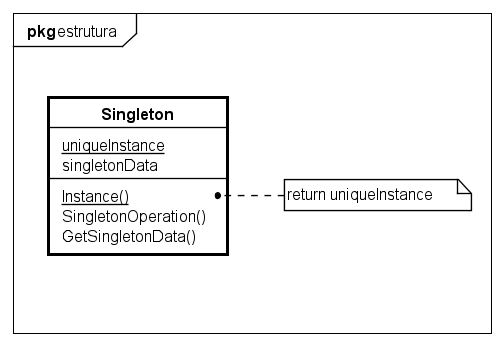
\includegraphics[scale=0.6]{5_padroes-contexto-funcional/5.1_criacionais/5.1.5_singleton/singleton_estrutura.png}
	\end{center}
\end{figure}

\subsection*{Exemplo Orientado a Objetos}

Uma classe define as operações para realizar transações com 
uma base de dados. Como a instância dela é idêntica independente 
do cliente que a utiliza, não existe a necessidade de replicar 
essas instâncias pelo código. Ela pode ser transformada em 
um Singleton, o que faz com que toda classe que deseja fazer 
uma transação na base de dados apenas solicite uma instância 
e realize as operações. A definição da classe do exemplo 
pode ser vista na figura \ref{singleton_exemplo} e no 
código \ref{oosingleton}.

\begin{figure}[htb]
	\caption{\label{singleton_exemplo}Exemplo de Singleton}
	\begin{center}
	    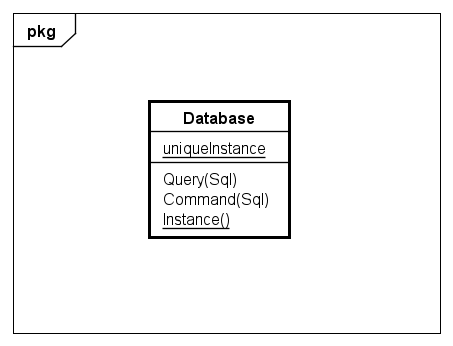
\includegraphics[scale=0.6]{5_padroes-contexto-funcional/5.1_criacionais/5.1.5_singleton/singleton_exemplo.png}
	\end{center}
\end{figure}

\begin{lstlisting}[caption={Singleton Orientação a Objetos},label=oosingleton]

class Database private(){
  def Query(sql : String) : Object = {
    //Execute query
    null
  }
  def Command(sql : String) : Unit = {
    //Execute command
  }
}

object Database {
  private var instance : Database = null

  def Instance() : Database = {
    if(instance == null){
      instance = new Database()
    }
    instance
  }
}

\end{lstlisting}

\subsection*{Contexto Funcional}

Em um contexto sem classes e objetos, 
um singleton poderia ser considerado como 
uma variável global, acessível por 
todo o programa. Essa ideia viola o conceito 
de função pura, já que uma função que acessa 
um singleton deixa de depender apenas de seus 
parâmetros. Para o caso em que o Singleton 
armazene algum estado, o conceito de imutabilidade 
também precisaria ser violado, já que o 
valor que armazena o Singleton precisaria ser 
mutável para ser alterado de dentro de uma 
função. Com isso, não existe uma implementação 
equivalente ao Singleton no contexto funcional.

% ----------------------------------------------------------
% ESTRUTURAIS
% ----------------------------------------------------------
%\chapter{Padrões Estruturais}

\chapter{Padrões Estruturais}

\section{Adapter}

Quando a interface de uma classe, objeto ou biblioteca não 
é compatível com a interface atual do cliente que deseja 
utilizar essa interface, o padrão Adapter fornece uma 
solução que evita a refatoração e a dependência da interface 
do cliente para a interface desejada.

Existem duas formas de realizar essa adaptação. Um Adapter 
de classe (Figura \ref{adapter_struct}), que só é possível 
para linguagens que implementam herança múltipla, implementa 
uma classe que herda tanto da classe que representa a interface 
da aplicação quanto da classe que representa a interface que 
deseja ser utilizada. 

\begin{figure}[htb]
	\caption{\label{adapter_struct}Estrutura do Adapter de Classe}
	\begin{center}
	    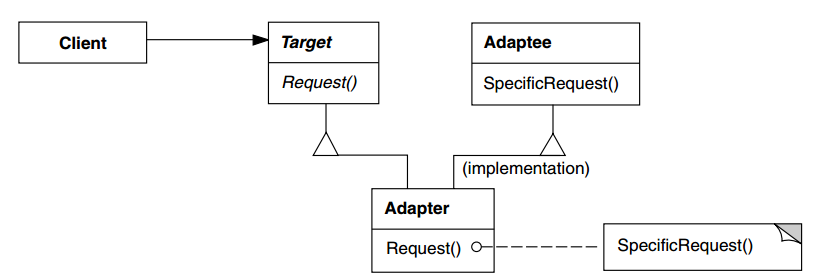
\includegraphics[scale=0.5]{5_padroes-contexto-funcional/5.2_estruturais/5.2.1_adapter/diagram2.png}
	\end{center}
\end{figure}

Já o Adapter de Objeto (Figura \ref{adapter_alt_struct}) 
herda apenas da classe que representa 
a interface da aplicação e reimplementa a operação desejada 
de forma que, após adaptar para a operação para a interface 
desejada, delega a realização da mesma para um objeto que 
implemente essa interface.

\begin{figure}[htb]
	\caption{\label{adapter_alt_struct}Estrutura do Adapter de Objeto}
	\begin{center}
	    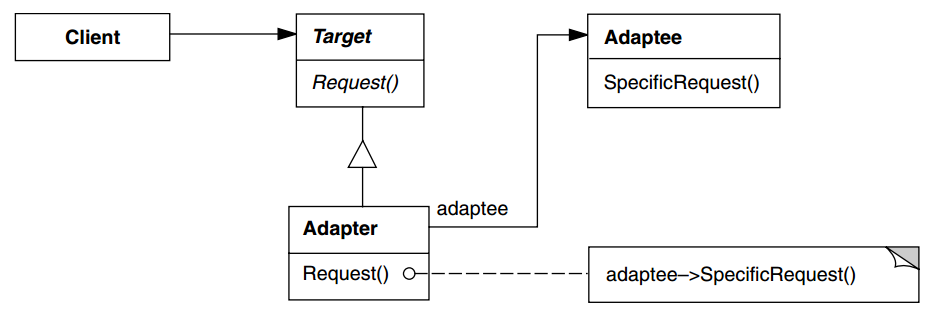
\includegraphics[scale=0.4]{5_padroes-contexto-funcional/5.2_estruturais/5.2.1_adapter/diagram.png}
	\end{center}
\end{figure}

\subsection*{Exemplo Orientado a Objetos}

Como exemplo é apresentada uma ferramenta gráfica 
que permite a edição de diversos objetos gráficos 
simples, entre eles linhas e polígonos. Porém, 
a aplicação deseja também editar elementos textuais, 
que são mais complexos de se gerenciar. Como já existem 
ferramentas prontas para gerenciar esse tipo de 
elemento, é desejado reutilizá-lo. Já que as 
ferramentas prontas não foram feitas pensando na 
aplicação de ferramenta gráfica do exemplo, uma 
classe Adapter é implementada para adaptar a 
ferramenta textual para a aplicação que deseja 
utilizá-la. Para esse exemplo, é utilizada a 
abordagem de Adapter de objeto, onde um objeto 
do tipo da ferramenta textual é armazenado. O 
diagrama de classes do exemplo pode ser visto na 
figura \ref{adapter_exemplo}, enquanto a 
implementação em código pode ser vista no código 
\ref{ooadapter}.


\begin{figure}[htb]
	\caption{\label{adapter_exemplo}Exemplo de Adapter}
	\begin{center}
	    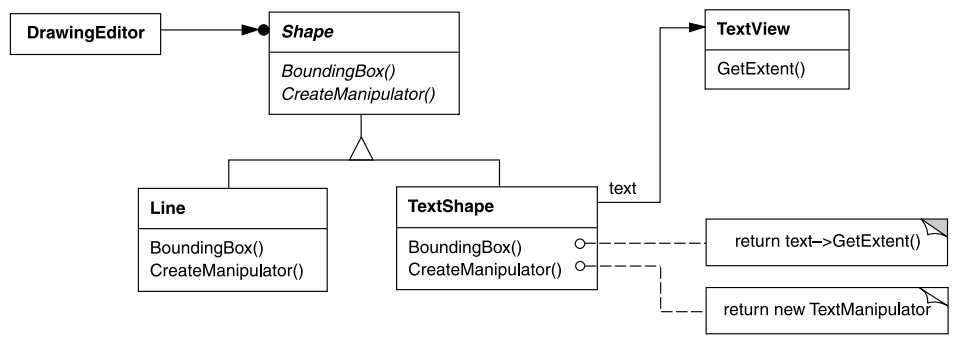
\includegraphics[scale=0.45]{5_padroes-contexto-funcional/5.2_estruturais/5.2.1_adapter/exemplo_adapter.png}
	\end{center}
\end{figure}


\begin{lstlisting}[caption={Adapter Orientado a Objetos},label=ooadapter]

class Shape(
	var bottomLeft : Point, 
	var topRight : Point
) {

}

class Line() extends Shape {

}

class TextShape(
	textView : TextView,
	var bottomLeft : Point, 
	var topRight : Point) extends Shape {

}

class TextView(
	var x : Coord, var y : Coord,
	var width : Coord : var height : Coord
) {


}


\end{lstlisting}



\subsection*{Contexto Funcional}

Existem duas formas simples de implementar um Adapter em uma linguagem 
funcional: usando funções de alta ordem e composição de funções.

Através de funções de alta ordem é possível passar por parâmetro, 
quando necessário, uma função que adapta o valor definido no cliente 
para o valor que precisa ser recebido pela função incompatível. O 
problema dessa abordagem é a necessidade do cliente conhecer a função 
Adapter e a biblioteca.

Já com composição de funções, uma função composta da função Adapter 
e da função incompatível é fornecida para o cliente, que sem precisar 
saber que está usando um Adapter, pode realizar a operação incompatível 
sem problemas.

\begin{lstlisting}[caption={Adapter Funcional},label=fpadapter]
    

    
\end{lstlisting}
\section{Bridge}

\begin{figure}[htb]
	\caption{\label{bridge_struct}Estrutura do Bridge}
	\begin{center}
	    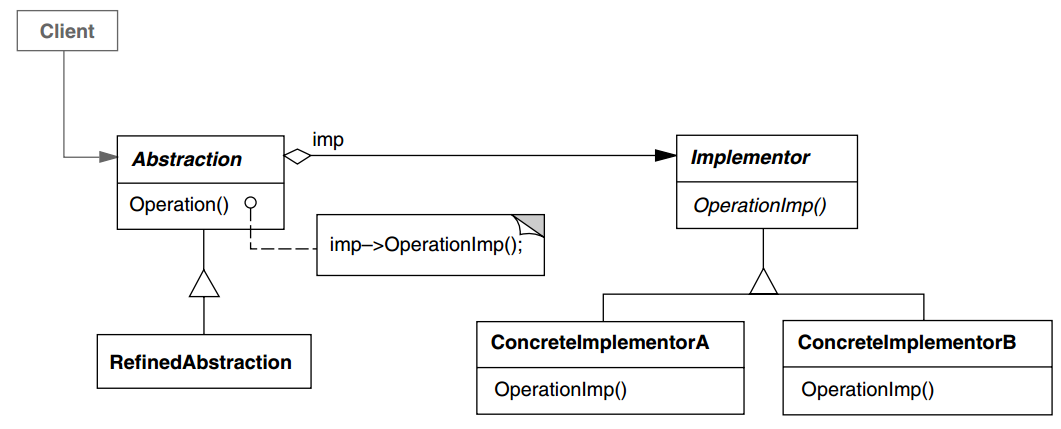
\includegraphics[scale=0.4]{5_padroes-contexto-funcional/5.2_estruturais/5.2.2_bridge/diagram.png}
	\end{center}
\end{figure}

Exemplo Orientado a Objetos:

\begin{lstlisting}[caption={Bridge Orientado a Objetos},label=oobridge]



\end{lstlisting}

Contexto Funcional:


\begin{lstlisting}[caption={Bridge Funcional},label=fpbridge]
    

    
\end{lstlisting}
\section{Composite}

Esse padrão fornece uma estrutura de objetos 
organizados como uma árvore, representados 
por uma hierarquia parte-todo. 
Ele torna possível tratar tanto o conjunto 
quanto os objetos individuais de forma 
uniforme, sem que seja necessário conhecer 
os elementos pertencentes a um conjunto para 
tratá-lo.

A figura \ref{composite_struct} demonstra a 
estrutura do padrão, onde uma interface Component 
define tanto um objeto nó, representado pela 
classe Composite, quanto um objeto folha, 
representado pela classe Leaf. Os elementos 
filhos da classe Composite são todos instâncias 
de Component, o que faz com que a classe não 
saiba se seus filhos são outros objetos compostos 
ou se são objetos folha.

\begin{figure}[htb]
	\caption{\label{composite_struct}Estrutura do Composite}
	\begin{center}
	    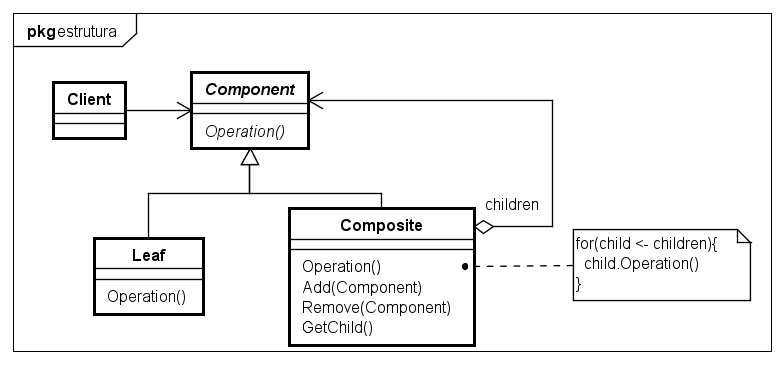
\includegraphics[scale=0.5]{5_padroes-contexto-funcional/5.2_estruturais/5.2.3_composite/composite_estrutura.png}
	\end{center}
\end{figure}

\subsection*{Exemplo Orientado a Objetos}

Como exemplo, é apresentada uma ferramenta gráfica 
onde o usuário pode agrupar diversas formas e 
elementos 
para formar diagramas maiores e mais complexos. 
Apesar do usuário tratar esses diagramas como um 
único elemento gráfico, a aplicação precisa levar 
em consideração todos os elementos dos quais ele 
é composto. Dessa forma, o padrão Composite permite 
abstrair os elementos menores, tratando o elemento 
composto como algo único, da mesma forma que 
são tratados os elementos não compostos. A figura 
\ref{composite_exemplo} demonstra o diagrama de 
classes para esse exemplo, enquanto o código 
\ref{oocomposite} traz um exemplo de implementação.

\begin{figure}[htb]
	\caption{\label{composite_exemplo}Exemplo de Composite}
	\begin{center}
	    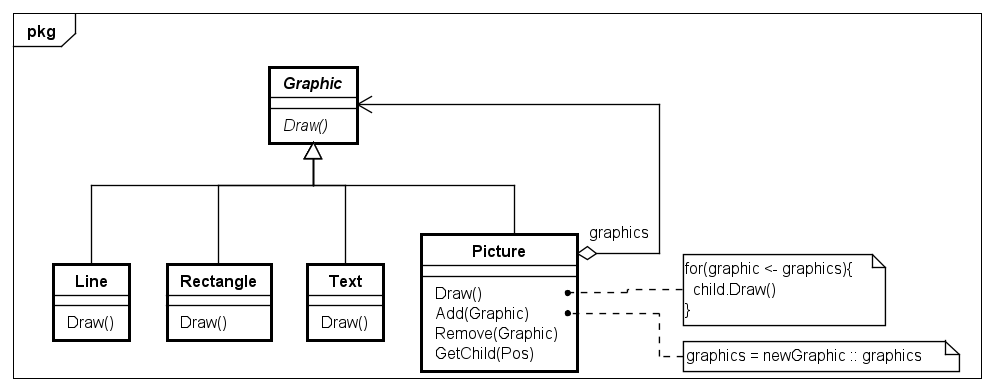
\includegraphics[scale=0.5]{5_padroes-contexto-funcional/5.2_estruturais/5.2.3_composite/composite_exemplo.png}
	\end{center}
\end{figure}

\begin{lstlisting}[caption={Composite Orientado a Objetos},label=oocomposite]

trait Graphic {
  def Draw();
}

class Picture extends Graphic {
  private var graphics : List[Graphic] = List()

  def Draw() : Unit = {
    graphics.foreach(f => f.Draw())
  }

  def Add(graphic: Graphic): Unit = {
    graphics = graphic :: graphics
  }

  def Remove(graphic: Graphic) : Unit = {
    graphics = graphics.filter(g => g != graphic)
  }

  def GetChild(pos : Int) : Graphic = graphics(pos)
}

class Text extends Graphic {
  def Draw() : Unit = {
    //Desenha o elemento na tela
  }
}

class Rectangle extends Graphic {
  def Draw() : Unit = {
    //Desenha o elemento na tela
  }
}

class Line extends Graphic {
  def Draw() : Unit = {
    //Desenha o elemento na tela
  }
}

\end{lstlisting}

\subsection*{Contexto Funcional}

O código \ref{fpcomposite} demonstra como é 
possível declarar a estrutura do padrão Composite 
utilizando funções de alta ordem. A função 
Draw, definida na linha 2, é equivalente à função 
Draw da classe Picture do exemplo orientado a 
objetos. A diferença é que ela recebe como parâmetro 
uma lista de funções e retorna uma nova função, 
com a mesma assinatura, que executa todas as 
funções da lista. As funções DrawLine, DrawRectangle 
e DrawText, definidas nas linhas 5, 10 e 15, 
respectivamente, são equivalentes aos elementos 
folha da estrutura de árvore proposta pelo 
Composite. Elas recebem como parâmetro todos 
os valores necessários para desenhar os elementos 
gráficos e retornam uma função para 
desenhá-los.

As funções retornadas são adicionadas a uma 
lista que deve ser passada para a função Draw. 
Como a assinatura de Draw é igual à das funções 
que ela recebe, uma nova chamada de Draw pode 
conter tanto "funções folha" quanto funções 
que são resultado da chamada de Draw. Isso 
favorece a vantagem do padrão Composite de 
permitir que toda a estrutura seja tratada 
de forma indefinida, sem que a função 
cliente precise saber se está tratando de um 
grupo de elementos ou de um elemento apenas. 

\begin{lstlisting}[caption={Composite Funcional},label=fpcomposite]
    
def Draw(functions : List[() => Unit]) : () => Unit =
  () => functions.foreach((function) => function())

def DrawLine(length : Int) : () => Unit =
  () => {
    // Desenha linha
  }

def DrawRectangle(width : Int, height : Int) : () => Unit =
  () => {
    // Desenha retângulo
  }

def DrawText(text : String) : () => Unit =
  () => {
    // Escreve texto
  }
    
\end{lstlisting}

O código \ref{fpcompositeapp} demonstra a 
aplicação do padrão. O valor DrawGraphics, 
definido na linha 2, é o resultado da aplicação 
de Draw para uma lista contendo uma função que 
desenha uma linha e uma função que desenha 
um retângulo. Já o valor DrawAllText, definido 
na linha 7, é definida através de duas funções 
que desenham texto. Na linha 12, o valor 
DrawEverything é definido a partir das funções 
armazenadas nos valores DrawGraphics e 
DrawAllText. Ao ser executado, ele executará 
também todas as funções definidas anteriormente 
tratando todo o conjunto como um único elemento, 
da forma como o padrão Composite propõe.

\begin{lstlisting}[caption={Aplicação do Composite Funcional},label=fpcompositeapp]
    
val DrawGraphics : () => Unit = Draw(
  List(
    DrawLine(5),
    DrawRectangle(4, 5)))

val DrawAllText : () => Unit = Draw(
  List(
    DrawText("Text 1"),
    DrawText("Text 2")))

val DrawEverything : () => Unit = Draw(
  List(
    DrawGraphics,
    DrawAllText))
    
\end{lstlisting}
\subsection{Decorator}

O padrão Decorator permite adicionar responsabilidades a um 
objeto de forma dinâmica. Essa dinamicidade é alcançada 
substituindo a herança por uma agregação, permitindo que a 
classe decorada delegue responsabilidades para as classes que 
a extendem. As classes de extensão implementam uma mesma 
interface que as classes decoradas e possuem um objeto dessa 
mesma classe entre seus atributos. Dessa forma, uma classe 
de extensão pode tanto referenciar outra classe de extensão 
quanto o objeto decorado, formando uma estrutura de pilha 
onde o elemento ao fundo é o objeto decorado que será o 
alvo das operações de todos os extensores presentes na 
estrutura.

O maior problema resolvido pelo Decorator é a grande 
quantidade de classes que deveriam existir caso houvessem 
muitas extensões para uma classe. O problema cresce ainda 
mais quando é necessário que essas funcionalidades mudem 
dinamicamente, gerando diversas combinações de grupos de 
funcionalidades possíveis.

\begin{figure}[htb]
	\caption{\label{fig_grafico}Estrutura do Decorator}
	\begin{center}
	    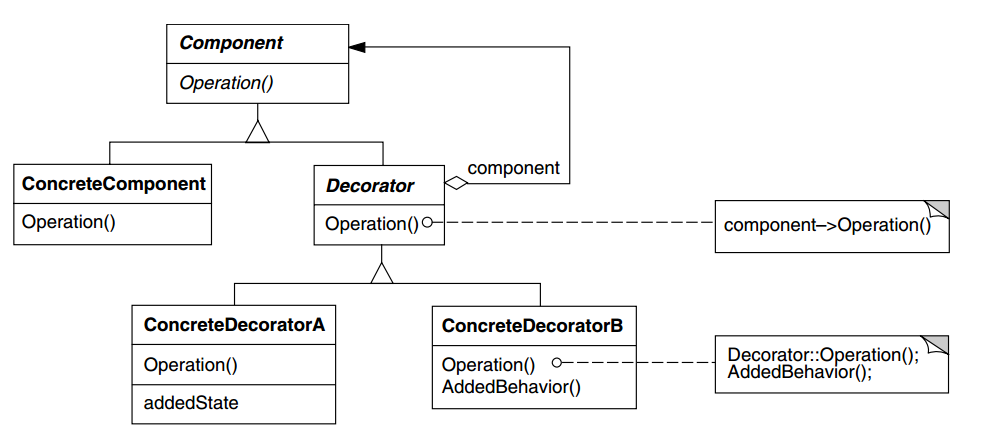
\includegraphics[scale=0.5]{5_padroes-contexto-funcional/5.2_estruturais/5.2.4_decorator/diagram.png}
	\end{center}
\end{figure}

Exemplo Orientado a Objetos:

\begin{lstlisting}[caption={Decorator Orientado a Objetos},label=oodecorator]



\end{lstlisting}

Contexto Funcional:

O mesmo objetivo é alcançado de forma simples através de 
composição de funções. Caso um valor precise ser decorado 
com diversas funções, uma função recebe esse valor como 
parâmetro e uma lista com todas as funcionalidades que irão 
estendê-lo. Essas funções são então chamadas uma por uma, 
gerando também uma pilha de chamadas que finalmente 
retorna o resultado da combinação de todas as operações.

\begin{lstlisting}[caption={Decorator Funcional},label=fpdecorator]
    

    
\end{lstlisting}
\section{Façade}

Quando um subsistema possui muitas interfaces 
de acesso às suas funcionalidades, o acesso de 
classes clientes de outros subsistemas a ele 
torna-se descentralizado, aumentando a dependência 
entre os dois sistemas. Para minimizar esse problema, 
o padrão Façade fornece uma interface generalizada 
para todo o subsistema, de forma que as classes 
clientes possam comunicar-se apenas com um ponto 
de entrada. A Figura \ref{facade_struct} demonstra 
o padrão, na qual uma classe Façade, que é o ponto de 
acesso ao subsistema, possui uma referência para 
os componentes que antes eram diretamente acessíveis.\cite{gamma:1995}

\begin{figure}[htb]
	\caption{\label{facade_struct}Estrutura do Façade.}
	\begin{center}
	    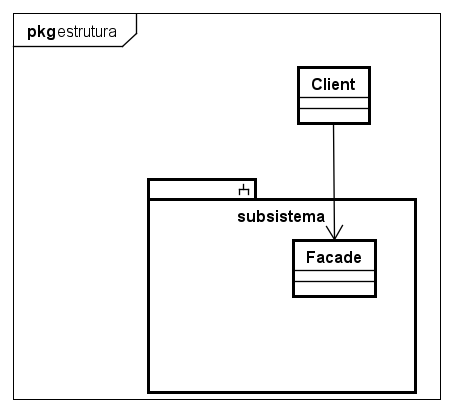
\includegraphics[scale=0.4]{5_padroes-contexto-funcional/5.2_estruturais/5.2.5_facade/facade_estrutura.png}
	\end{center}
\end{figure}

\subsection*{Exemplo Orientado a Objetos}

Como exemplo de uso do Façade, pode-se considerar 
um compilador que oferece diversas funcionalidades. 
Essas funcionalidades são apresentadas no diagrama 
de classes da Figura \ref{facade_exemplo}, representadas 
pelas classes Scanner, Parser, ProgramNodeBuilder e 
CodeGenerator. Por mais que alguns clientes desejem 
acessar essas funcionalidades diretamente, a maioria 
deseja apenas compilar seu programa, sem importar-se 
com as etapas necessárias para isso. Assim, ao invés de 
criar uma dependência entre o cliente e as 
funcionalidades, a classe Compiler fornece um ponto 
de acesso a todas elas, permitindo que um cliente 
que deseja apenas compilar seu código possa fazer 
isso diretamente. O Código \ref{oofacade} demonstra 
a implementação desse exemplo.

\begin{figure}[htb]
	\caption{\label{facade_exemplo}Exemplo de Façade.}
	\begin{center}
	    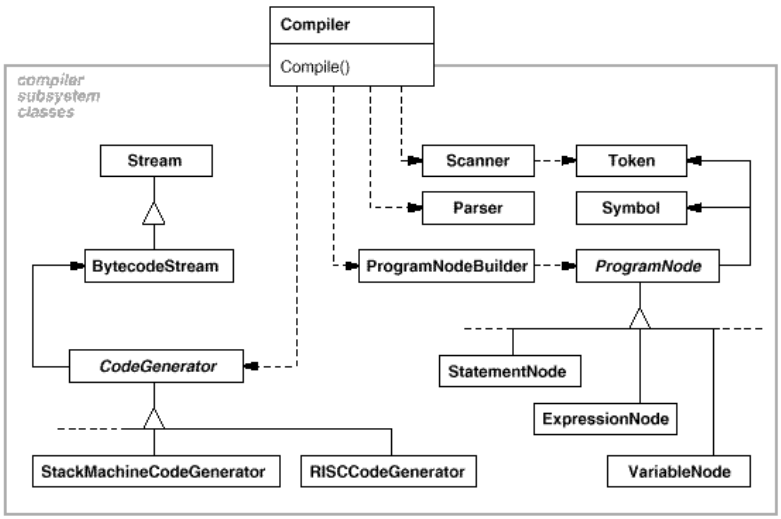
\includegraphics[scale=0.4]{5_padroes-contexto-funcional/5.2_estruturais/5.2.5_facade/facade_exemplo.png}
	\end{center}
\end{figure}


\begin{lstlisting}[caption={Façade Orientado a Objetos.},label=oofacade]

class Scanner(val input : Stream[String]) {
  def Scan() : Token = {
    //Recupera token na stream de código fonte
  }
}

class Parser {
  def Parse(scanner : Scanner, builder : ProgramNodeBuilder) : SyntacticTree[ProgramNode] = {
    //Retorna a árvore de análise
  }
}

class ProgramNodeBuilder(var rootNode : ProgramNode) {
  // Possui os métodos para criação dos nós do programa
}

class CodeGenerator() {
  // Possui os métodos para gerar o código de máquina do programa
  def Traverse(rootNode : ProgramNode) : Stream[Byte] = {
    // Percorre a árvore e gera o bytecode
  }
}

class Compiler {
  def Compile(input : Stream[String]) : Stream[Byte] = {
    val scanner = new Scanner(input)
    val programNodeBuilder = new ProgramNodeBuilder(null)
    val parser = new Parser();

    parser.Parse(scanner, programNodeBuilder);

    val codeGenerator = new CodeGenerator();
    val parseTree = programNodeBuilder.rootNode;

    codeGenerator.Traverse(parseTree);
  }
}

\end{lstlisting}

\subsection*{Contexto Funcional}

Esse padrão pode ser implementado de duas formas: 
definindo um módulo que é utilizado como ponto de 
acesso para outros módulos ou definindo uma 
função dentro de um módulo que é um ponto de 
acesso para outras funções não exportadas do 
mesmo módulo. Independente da forma utilizada, 
a função Compile, que é o ponto de acesso, permanece 
a mesma. Ela pode ser vista no Código \ref{facadecompile}. 

Para que essa função seja implementada de forma 
funcional, a implementação vista no Código \ref{oofacade} 
foi alterada para que seja utilizada uma composição 
de funções. Na linha 5, a função Scan é chamada, 
seu resultado é passado para a função Parse, cujo 
resultado é passado para a função Traverse. Essa sim, 
retorna a \textit{stream} de \textit{bytes} com o 
código compilado do programa.

\begin{lstlisting}[caption={Função de acesso Compile.},label=facadecompile]
    
object Compiler {

  def Compile(input: Stream[String]): Stream[Byte] = {
    (Traverse compose Parse compose Scan) (input)
  }
  
}
    
\end{lstlisting}

O Código \ref{facademodules} demonstra o primeiro caso, 
no qual as operações utilizadas pela função Compile são 
definidas em módulos separados. Apenas o módulo 
Compiler precisa conhecer e importar essas funções.

\begin{lstlisting}[caption={Função de acesso Compile.},label=facademodules]
    
object Scanner{
  private def Scan(input : Stream[String]) : Scanner = 
    // Faz o scan do código fonte
}

object Parser{
  private def Parse(scanner : Scanner)
  : ProgramNodeBuilder = 
    // Gera a árvore abstrata sintática com os tokens
}

object CodeGenerator{
  private def Traverse(builder : ProgramNodeBuilder) : Stream[Byte] = 
    // Percorre a árvore para gerar o código de máquina
}

\end{lstlisting}

Para o segundo exemplo, o Código \ref{facadepvtfunc} define 
as funções como membros não exportados do módulo Compiler. 
Dessa forma, o módulo cliente não conseguirá acessá-los, 
precisando acessar suas funcionalidades apenas através da 
função Compile.

\begin{lstlisting}[caption={Função de acesso Compile.},label=facadepvtfunc]
    
  // módulo Compiler    

  private def Scan(input : Stream[String]) : Scanner = 
    // Faz o scan do código fonte

  private def Parse(scanner : Scanner)
  : ProgramNodeBuilder = 
    // Gera a árvore abstrata sintática com os tokens

  private def Traverse(builder : ProgramNodeBuilder) : Stream[Byte] = 
    // Percorre a árvore para gerar o código de máquina
    
\end{lstlisting}

\begin{comment}
\subsection*{Vantagens e Desvantanges}

A implementação funcional desse padrão não apresenta 
vantagens ou desvantagens, tendo em vista que ela apenas 
depende da forma como a linguagem separa ou agrupa 
suas implementações - seja através de classes ou módulos. 
\end{comment}
\section{Flyweight}

O padrão Flyweight permite economizar o espaço em memória 
da aplicação ao fornecer uma instância compartilhada de 
uma classe, para que ela não precise ser instanciada 
diversas vezes.

\begin{figure}[htb]
	\caption{\label{flyweight_struct}Estrutura do Flyweight}
	\begin{center}
	    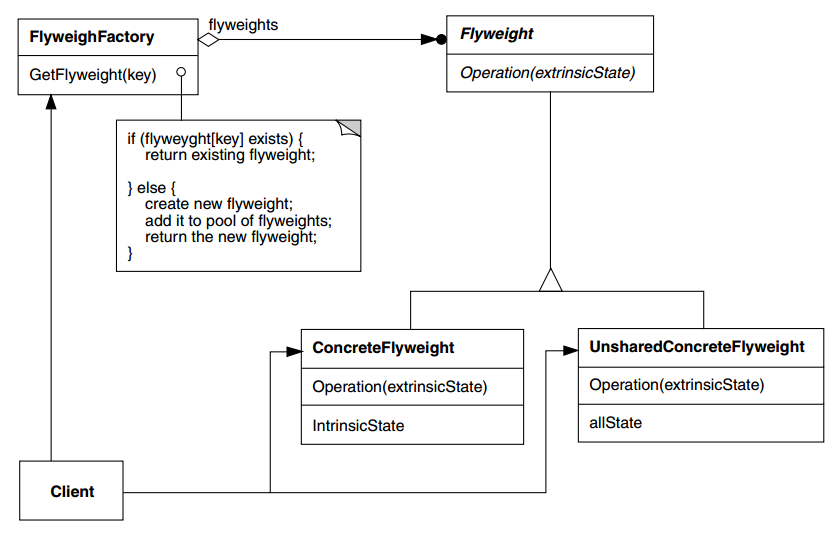
\includegraphics[scale=0.5]{5_padroes-contexto-funcional/5.2_estruturais/5.2.6_flyweight/diagram.png}
	\end{center}
\end{figure}

Exemplo Orientado a Objetos:

\begin{lstlisting}[caption={Flyweight Orientado a Objetos},label=ooflyweight]



\end{lstlisting}

Contexto Funcional:

A ideia do Flyweight assemelha-se à de memoização, onde o 
retorno de uma função pura é armazenado para que seu valor 
não precise ser recalculado quando os mesmos parâmetros 
são passados. Essa abordagem só é possível para funções 
puras pois, caso ocorram efeitos colaterais ou a função 
dependa de dados externos, o resultado pode ser diferente 
para os mesmos parâmetros, gerando um resultado não 
confiável.

Apesar da ideia de memoização parecer mais focada no tempo 
de execução no que no espaço em memória, dependendo da 
implementação é possível economizar ambos.

\begin{lstlisting}[caption={Flyweight Funcional},label=fpflyweight]
    

    
\end{lstlisting}
\section{Proxy}

O padrão Proxy adiciona uma camada de acesso 
a um objeto, fazendo com que qualquer interação 
com o objeto Proxy seja controlada antes de ser 
repassada para o objeto real. Existe mais 
de uma motivação para seu uso, apesar 
da estrutura do padrão, 
apresentada na Figura \ref{proxy_struct},  
permanecer a mesma. Essas motivações 
podem ser divididas em três grupos de 
proxy: remoto, virtual e de proteção. \cite{gamma:1995}

Um proxy remoto pode ser utilizado como um 
representante de um objeto, servindo como um 
intermediário e armazenando dados que devem 
ser repassados para o objeto real. Já um 
proxy virtual armazena informações sobre 
um objeto de forma que ele possa ser criado 
apenas quando for necessário, economizando 
espaço ou tempo de execução. Por fim, um 
proxy de proteção pode controlar o acesso 
a um objeto, exigindo que um objeto cliente 
precise cumprir algum requisito antes de 
acessar o objeto real. \cite{gamma:1995}

\begin{figure}[htb]
	\caption{\label{proxy_struct}Estrutura do Proxy.}
	\begin{center}
	    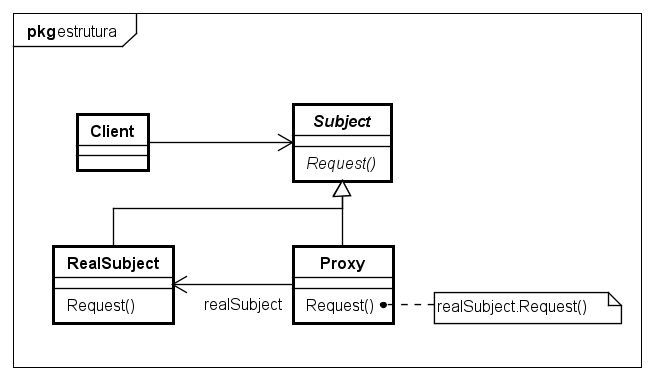
\includegraphics[scale=0.5]{5_padroes-contexto-funcional/5.2_estruturais/5.2.7_proxy/proxy_estrutura.png}
	\end{center}
\end{figure}

\subsection*{Exemplo Orientado a Objetos}

Como exemplo de Proxy podem ser utilizadas 
imagens que são incluídas em editores de 
texto. É desejado que um documento seja aberto 
rapidamente e o carregamento das imagens 
presentes nele pode causar uma lentidão 
desnecessária. Para isso, é criado um objeto 
Proxy que armazena em seus atributos as 
informações necessárias, como o caminho 
para a imagem e seu posicionamento no 
documento. Quando o documento termina de 
ser aberto, as imagens são carregadas de 
fato através de seus proxys. Esse é um 
exemplo de proxy virtual, seu diagrama de 
classes pode ser visto na Figura \ref{proxy_exemplo} 
e a implementação no Código \ref{ooproxy}.

\begin{figure}[htb]
	\caption{\label{proxy_exemplo}Exemplo de Proxy.}
	\begin{center}
	    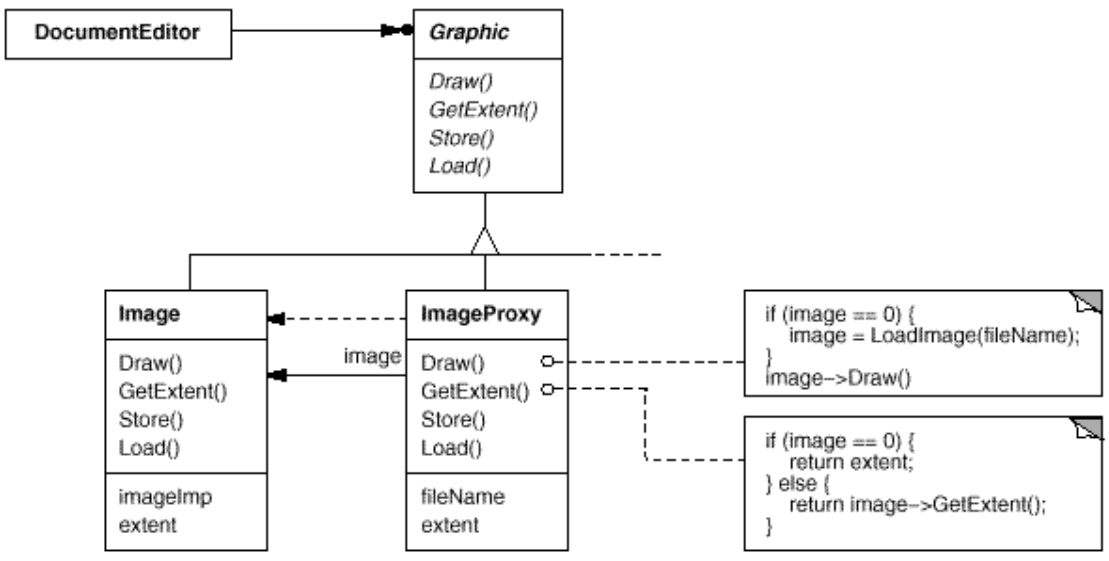
\includegraphics[scale=0.5]{5_padroes-contexto-funcional/5.2_estruturais/5.2.7_proxy/proxy_exemplo.png}
	\end{center}
\end{figure}

\begin{lstlisting}[caption={Proxy Orientado a Objetos.},label=ooproxy]

trait Graphic {
  def Draw(point : Point)
  def GetExtent() : Point
  def Store(ostream : Stream[Byte])
  def Load(istream : Stream[Byte])
}

class Image (private val filename : String) extends Graphic {

  private var extent : Point = new Point

  def Draw(point: Point): Unit = {
    //Desenha imagem na tela
  }

  def GetExtent(): Point = extent

  def Store(ostream: Stream[Byte]): Unit = {
    //Salva imagem em um arquivo
  }

  def Load(istream: Stream[Byte]): Unit = {
    //Carrega imagem de um arquivo
  }
}

class ImageProxy(var filename : String, var extent : Point) extends Graphic {

  private var image : Image = null

  override def Draw(point: Point): Unit = {
    if(image == null){
      image = new Image(filename)
    }
    image.Draw(point)
  }

  override def GetExtent(): Point = {
    if(image==null){
      image = new Image(filename)
    }
    image.GetExtent()
  }

  def Store(ostream: Stream[Byte]): Unit = {
    //Salva imagem em um arquivo
  }

  def Load(istream: Stream[Byte]): Unit = {
    //Carrega imagem de um arquivo
  }
}

\end{lstlisting}

\subsection*{Contexto Funcional}

Para implementar um Proxy, uma função do 
editor de documentos pode receber como 
parâmetro uma função cuja assinatura seja 
a mesma do método Draw no exemplo orientado 
a objetos. Dessa forma, tanto é possível 
receber a função real quanto a função 
intermediária, sem que a função cliente 
esteja ciente de qual está sendo utilizada. 
A função intermediária, assim como nos 
métodos da classe intermediária no exemplo 
orientado a objetos, executará a função 
real, de acordo com o tipo de proxy que 
deve ser implementado. 

No Código \ref{fpproxy}, a função intermediária 
DrawImageProxy, definida na linha 6, chama a 
função real DrawImage, definida na linha 2. 
A função EditorFunction, definida na linha 11, 
representa uma função cliente qualquer que 
precisa desenhar a imagem. Ao invés de chamar 
diretamente a função DrawImage, ela recebe 
como parâmetro uma função com a mesma assinatura, 
para que seja possível que ela receba a função 
Proxy.

Existem algumas desvantagens quanto a essa 
implementação. Não é possível que haja 
estado atrelado ao Proxy, pois para que 
esse estado seja refletido na função 
cliente, é necessário que uma nova função, 
atualizada com o novo estado do Proxy, seja 
retornada pelas funções intermediárias. 
Isso faz com que o cliente precise gerenciar 
a mudança do Proxy, violando 
um dos propósitos do padrão. 

\begin{lstlisting}[caption={Proxy Funcional.},label=fpproxy]
    
def DrawImage(point : Point, image : Image) : Image = {
  // Desenha a imagem
}

def DrawImageProxy(point : Point, image : Image) : Image = {
  // Proxy realiza as operações necessárias antes de desenhar a imagem
  DrawImage(point, image)
}

def EditorFunction(filename : String, Draw : (Point, Image) => Image) : Unit = {
  //...
  img = Draw(point, img)
  //...
}
    
\end{lstlisting}

% ----------------------------------------------------------
% COMPORTAMENTAIS
% ----------------------------------------------------------
%\chapter{Padrões Comportamentais}

\chapter{Padrões Comportamentais}

\section{Chain of Responsibility}

Chain of Responsability propõe criar uma estrutura para 
tratar solicitações feitas por um objeto cliente. As classes 
que tratam as solicitações são chamadas de \textit{handlers}. 
Uma solicitação é passada adiante por uma cadeia de 
\textit{handlers} até que seja tratada ou 
até que a cadeia chegue ao fim e a solicitação 
não possa ser atendida, retornando uma indicação 
de que a solicitação não pôde ser atendida.

Essa abordagem permite desacoplar os clientes das classes 
que tratam as solicitações e permite que os \textit{handlers} 
sejam definidos dinamicamente. Por outro lado, pode não ser 
possível prever se uma solicitação de um cliente será atendida, 
caso o \textit{handler} adequado não esteja na cadeia. A 
estrutura do padrão pode ser vista na figura \ref{chain_struct}.

\begin{figure}[htb]
	\caption{\label{chain_struct}Estrutura do Chain of Responsibility}
	\begin{center}
	    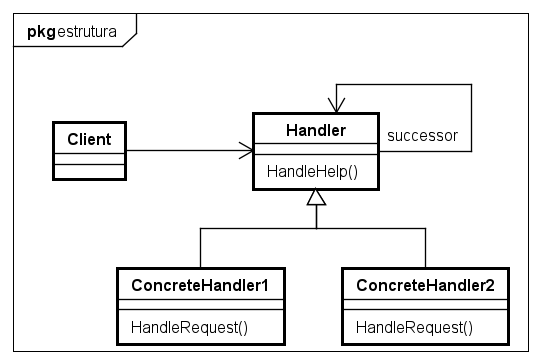
\includegraphics[scale=0.5]{5_padroes-contexto-funcional/5.3_comportamentais/5.3.01_chain-of-responsibility/chainofresponsibility_struct.png}
	\end{center}
\end{figure}

\subsection*{Exemplo Orientado a Objetos}

O exemplo do Chain of Responsibility traz um recurso 
de \textit{help} utilizado nos componentes de uma 
interface gráfica. O recurso é sensível ao contexto, 
bastando que o usuário solicite a ajuda no local 
desejado. O objeto que fornece a ajuda não é 
conhecido pelos objetos dos \textit{widgets} da 
interface, ele pertence a uma cadeia que é 
percorrida sempre que o usuário solicita 
a ajuda. A figura \ref{chain_exemplo} e o código 
\ref{oochresponsibility} demonstram esse exemplo.

\begin{figure}[htb]
	\caption{\label{chain_exemplo}Exemplo de Chain of Responsibility}
	\begin{center}
	    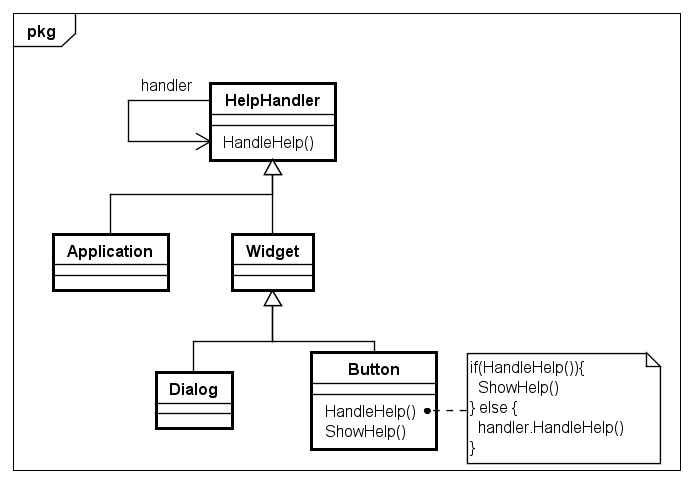
\includegraphics[scale=0.5]{5_padroes-contexto-funcional/5.3_comportamentais/5.3.01_chain-of-responsibility/chainofresponsibility_exemplo.png}
	\end{center}
\end{figure}

\begin{lstlisting}[caption={Chain of Responsibility Orientação a Objetos},label=oochresponsibility]

class HelpHandler(handler: HelpHandler = null, topic : Topic.Value = Topic.NO_HELP_TOPIC) {

  private var _handler : HelpHandler = handler
  private var _topic : Topic.Value = topic

  def HasHelp(): Boolean = {
    _topic != Topic.NO_HELP_TOPIC
  }

  def SetHandler(handler : HelpHandler, topic : Topic.Value) : Unit = {
    this._handler = handler
    this._topic = topic
  }

  def HandleHelp() : Unit = {
    if(_handler != null){
      _handler.HandleHelp()
    }
  }
}

class Widget(parent : Widget, topic : Topic.Value = Topic.NO_HELP_TOPIC)
  extends HelpHandler(parent, topic)
  
class Button(parent : Widget, topic: Topic.Value = Topic.NO_HELP_TOPIC)
  extends Widget(parent, topic) {

  override def HandleHelp(): Unit = {
    if(HasHelp()){
      //Oferece ajuda sobre o botão
    } else {
      parent.HandleHelp()
    }
  }
}

class Dialog(handler : HelpHandler, topic : Topic.Value = Topic.NO_HELP_TOPIC)
  extends Widget(null) {

  SetHandler(handler, topic)

  override def HandleHelp(): Unit = {
    if(HasHelp()) {
      // Oferece ajuda sobre dialog
    } else {
      handler.HandleHelp()
    }
  }
}

class Application(topic: Topic.Value)
  extends HelpHandler(null, topic) {

  override def HandleHelp(): Unit = {
    //Apresenta uma lista de tópicos de ajuda
  }
}

\end{lstlisting}

\subsection*{Contexto Funcional}

O Chain of Responsability encadeia funções que 
tratam solicitações, de forma que uma próxima 
função seja chamada quando a solicitação não 
pode ser tratada. É possível implementá-lo 
utilizando funções de alta ordem, onde um 
\textit{handler} é uma função, ao invés de 
uma classe, que armazena em uma \textit{closure} 
a função do próximo elemento da cadeia. 

O código \ref{fpchresponsibility} demonstra a 
criação dos \textit{handlers}. Na linha 2, a 
função HandleButton recebe como parâmetro um 
tópico e o próximo \textit{handler} da cadeia, 
assim como a classe Button do exemplo orientado 
a objetos. Ela retorna uma função que verifica 
se a solicitação pode ser tratada e, caso 
não seja, chama o \textit{handler} armazenado. 
A função HandleDialog, na linha 12, é 
implementada de forma análoga. Já a função 
HandleHelp, na linha 22, não recebe novos 
\textit{handlers}, oferecendo ajuda de forma 
genérica, da mesma forma que a classe 
Application do exemplo orientado a objetos.

\begin{lstlisting}[caption={Chain of Responsibility Funcional},label=fpchresponsibility]
    
def HandleButton(topic : Topic.Value, handler : () => Unit) : () => Unit = {
  () => {
    if(HasHelp(topic)){
      //Oferece ajuda sobre o botão
    } else {
      handler()
    }
  }
}

def HandleDialog(topic : Topic.Value, handler : () => Unit) : () => Unit = {
  () => {
    if(HasHelp(topic)){
      //Oferece ajuda sobre o dialog
    } else {
      handler()
    }
  }
}

def HandleHelp() : Unit = {
  //Apresenta uma lista de tópicos de ajuda
}
    
\end{lstlisting}

O código \ref{fpchainfunction} demonstra a criação 
da cadeia, onde as funções apresentadas anteriormente 
são criadas e encadeadas, criando a função 
ChainofResponsibility que será utilizada para 
tratar todas as solicitações.

\begin{lstlisting}[caption={Função Chain of Responsability},label=fpchainfunction]
    
val ChainofResponsibility: () => Unit = HandleButton(Topic.BUTTON,
  HandleDialog(Topic.DIALOG,
    HandleHelp))
      
\end{lstlisting}
\section{Command}

O padrão Command permite encapsular operações 
em objetos. Isso permite que seja mantido um 
histórico das operações realizadas, que seja 
criada uma sequência de operações a serem 
executadas e até mesmo que operações realizadas 
possam ser desfeitas.

Para alcançar isso, uma classe Command armazena o 
objeto alvo da operação e define uma operação 
de execução e uma de reversão, quando necessário. 
Uma outra classe pode ser responsável por armazenar 
uma coleção de \textit{commands}, mantendo o 
histórico ou sequência de operações. 

Esse padrão funciona como uma solução para definir 
\textit{callbacks}, ou seja, operações que podem ser 
predefinidas e executadas futuramente no código. Sua 
estrutura pode ser vista na imagem \ref{command_struct}.

\begin{figure}[htb]
	\caption{\label{command_struct}Estrutura do Command}
	\begin{center}
	    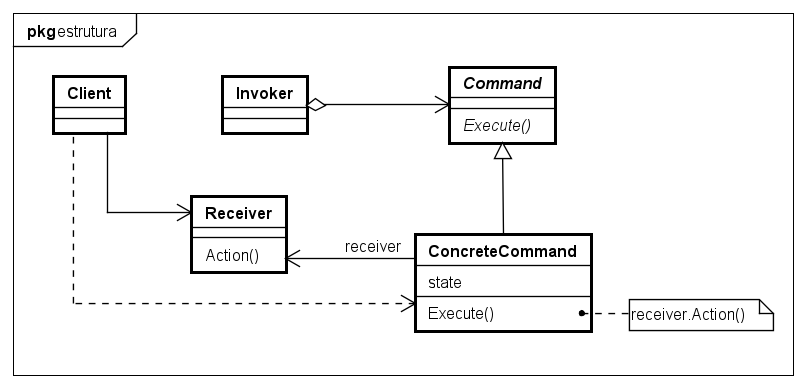
\includegraphics[scale=0.5]{5_padroes-contexto-funcional/5.3_comportamentais/5.3.02_command/command_struct.png}
	\end{center}
\end{figure}

\subsection*{Exemplo Orientado a Objetos}

O exemplo do Command traz um \textit{toolkit} para 
construção de interfaces de usuário, onde ao clicar 
ou realizar uma ação sobre botões e menus, uma 
operação deve ser executada. Porém, os botões e 
menus não devem conhecer essas operações, elas são 
definidas pelo desenvolvedor que utiliza os toolkits. 
Dessa forma, o padrão Command permite isolar as 
operações dos \textit{widgets}. O exemplo traz as 
operações PasteCommand, que tem como alvo um 
documento da aplicação, e OpenCommand, que tem como 
alvo o objeto da aplicação. Além disso, há um 
MacroCommand que permite executar uma sequência 
de comandos. O exemplo é apresentado no diagrama da 
imagem \ref{command_exemplo} e no código \ref{oocommand}.

\begin{figure}[htb]
	\caption{\label{command_exemplo}Exemplo de Command}
	\begin{center}
	    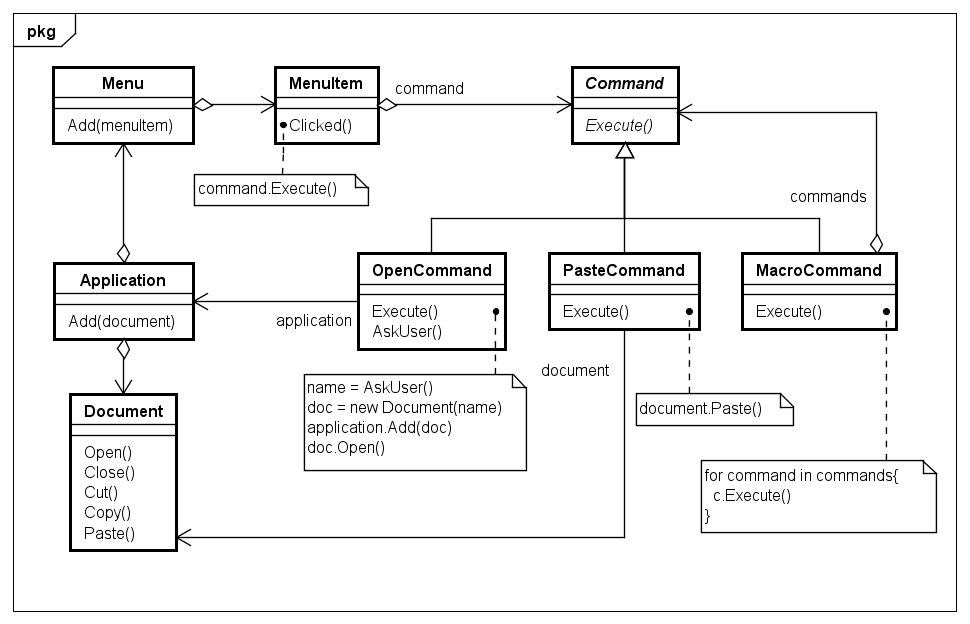
\includegraphics[scale=0.5]{5_padroes-contexto-funcional/5.3_comportamentais/5.3.02_command/command_exemplo.png}
	\end{center}
\end{figure}

\begin{lstlisting}[caption={Command Orientação a Objetos},label=oocommand]

abstract class Command {
  def Execute()
}

class OpenCommand(var application : Application) extends Command {
  def Execute(): Unit = {
    var name = AskUser()
    if(name != null){
      val document = new Document(name)
      application.Add(document)
      document.Open()
    }
  }

  def AskUser() : String = {
    //Solicita ao usuário o arquivo que será aberto
  }
}

class PasteCommand(var document : Document) extends Command {
  def Execute(): Unit = {
    document.Paste()
  }
}

class MacroCommand extends Command {

  private var commands : List[Command] = List()

  def Execute(): Unit = {
    commands.foreach(command => {
      command.Execute()
    })
  }
}
    
\end{lstlisting}

\subsection*{Contexto Funcional}

A a intenção do Command é encapsular operações 
em objetos. Com as funções de alta ordem da programação 
funcional, essa funcionalidade já é alcançada. 
Entretanto, existem duas particularidades 
do padrão Command que devem ser consideradas. 

O padrão encapsula, junto da operação, uma 
referência para o objeto alvo. Dessa forma, 
quando a operação é realizada, ocorre 
um efeito colateral, desencorajado 
no contexto funcional. Para evitar isso, o 
comando deve receber, ao ser executado, o 
valor alvo como parâmetro e retornar o 
valor atualizado.

A segunda particularidade é que o padrão 
também permite uma operação de desfazer. Como 
tanto a operação de fazer quanto a de desfazer 
são encapsuladas em um mesmo objeto, é necessário 
possuir um valor que armazena ambas as operações 
no contexto funcional. Isso pode ser feito 
através de uma tupla que armazena as duas 
operações.

O código \ref{fpcommand} demonstra uma implementação 
genérica do padrão no contexto funcional. Na linha 2, 
é definido um tipo Command que é uma tupla que 
armazena duas funções: fazer e desfazer. A função 
CreateCommand, na linha 4, é uma função auxiliar para 
a criação de um command. Caso não seja fornecida 
uma função de desfazer, a função é substituída por 
uma função identidade que recebe um valor como 
parâmetro e retorna esse mesmo valor.

As funções auxiliares Execute, na linha 12, e 
Unexecute, na linha 14, recebem como parâmetro o valor 
alvo e um comando. Elas executam a primeira e a 
segunda função armazenadas na tupla Command, 
respectivamente.

A função CommandMany, da linha 16, é uma função auxiliar 
para executar uma lista de \textit{commands}. Ela recebe 
como parâmetro um alvo, uma lista de \textit{commands} e 
uma operação que recebe um alvo e um comando. Essa 
operação genérica é utilizada para que essa função 
possa ser reaproveitada tanto para executar uma 
sequência de \textit{commands} quando desfazê-los. 
As funções ExecuteMany, na linha 20, e UnexecuteMany, 
na linha 23, chamam a função CommandMany passando 
como operação as função Execute e Unexecute, 
respectivamente.


\begin{lstlisting}[caption={Command Funcional},label=fpcommand]
    
type Command[A] = (A => A, A => A)

def CreateCommand[A](Do : (A) => A,
                     Undo : Option[(A) => A] = None) : Command[A] =
  (Do,
    Undo match {
      case Some(function) => function
      case None => (x) => x
  })

def Execute[A](target : A, command : Command[A]) : A = command._1(target)

def Unexecute[A](target : A, command: Command[A]) : A = command._2(target)

def CommandMany[A](target : A, commands : List[Command[A]], operation : (A, Command[A]) => A): A =
    if(commands.isEmpty) target
    else CommandMany(operation(target, commands.head), commands.tail, operation)

  def ExecuteMany[A](target : A, commands : List[Command[A]]) : A =
    CommandMany(target, commands, Execute)

  def UnexecuteMany[A](target : A, commands : List[Command[A]]) : A = {
    CommandMany(target, commands, Unexecute)
    
\end{lstlisting}

O código \ref{fpcommandexample} demonstra como o exemplo 
orientado a objetos poderia ser implementado a partir das 
funções auxiliares vistas. O valor ExecuteOpen, visto 
na linha 2, implementa a abertura de um documento em uma 
aplicação e retorna o estado atualizado dessa aplicação 
com o documento aberto. Já a função ExecutePaste, na 
linha 8, realiza a operação de colar um documento. 
O valor resultingApplication na linha 14 é o estado 
resultante da aplicação após a execução de ambos os 
comandos através da função auxiliar ExecuteMany.

\begin{lstlisting}[caption={Exemplo funcional de Command},label=fpcommandexample]
    
val ExecuteOpen = CreateCommand[Application](
  (target : Application) => {
    //Executa comando de abrir
  } : Application
)

val ExecutePaste = CreateCommand[Application](
  (target : Application) => {
    //Executa comando de colar
  }
)
  
val resultingApplication = ExecuteMany(application, List(ExecuteOpen, ExecutePaste))
    
\end{lstlisting}

\begin{comment}
\subsection*{Vantagens e Desvantagens}

O Command funcional consegue economizar classes, resumindo a 
complexidade do padrão à criação de uma tupla para os casos 
onde é desejado implementar a operação de desfazer. Para 
os casos onde isso não é necessário, a implementação se torna 
ainda mais simples, já que as funções de alta ordem em si 
já suprem a necessidade de encapsular operações. A grande 
desvantagem da implementação funcional é que a execução das 
operações se torna mais dependente do valor alvo. O valor 
atualizado sempre precisa ser repassado para o comando para 
que qualquer modificação feita anteriormente - seja por outro 
trecho da aplicação ou por um comando executado anteriormente - 
seja considerada durante a execução.
\end{comment}
\subsection{Interpreter}

De acordo com GoF, o Interpreter define uma representação para 
a gramática de uma linguagem e usa um interpretador para 
interpretar sentenças dessa linguagem.

Apesar da definição parecer específica, o padrão pode ser 
generalizado para qualquer hierarquia de classes, desde que 
não seja muito complexa. Dessa forma, o padrão permite 
interpretar essa hierarquia e realizar uma operação que 
dependa da forma como essas classes estão dispostas, por 
exemplo.

\begin{figure}[htb]
	\caption{\label{fig_grafico}Estrutura do Interpreter}
	\begin{center}
	    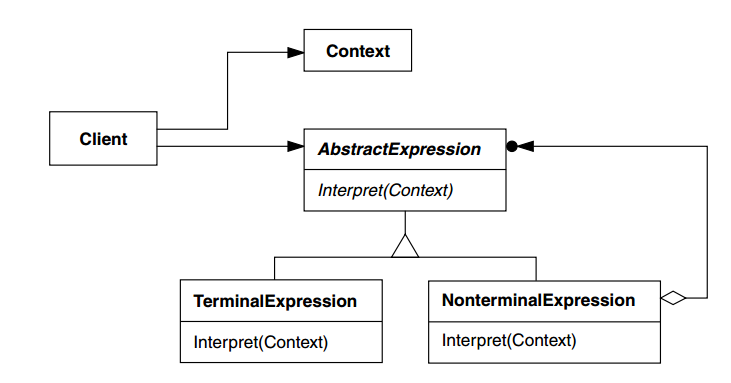
\includegraphics[scale=0.5]{5_padroes-contexto-funcional/5.3_comportamentais/5.3.03_interpreter/diagram.png}
	\end{center}
\end{figure}

Exemplo Orientado a Objetos:

\begin{lstlisting}[caption={Interpreter Orientação a Objetos},label=oointerpreter]


    
\end{lstlisting}

Contexto Funcional:

O próprio GoF cita pattern matching como um exemplo de 
aplicação do padrão Interpreter. Apesar de não ser um 
conceito necessariamente funcional, pattern matching costuma 
ser nativamente implementado por linguagens como Haskell e 
Scala. As linguagens funcionais também costumam implementar 
de forma mais simples tipos algébricos, que são definidos 
quase identicamente às gramáticas usadas para definir 
linguagens. Dessa forma, o que antes necessitaria de diversas 
classes e interfaces para uma hierarquia que não poderia 
ser muito complexa, pode ser traduzido como uma função 
que aproveita o pattern matching naturalmente para decidir 
e interpretar um valor definido através de um tipo abstrato.

\begin{lstlisting}[caption={Interpreter Funcional},label=fpinterpreter]
    

    
\end{lstlisting}
\section{Iterator}

\begin{figure}[htb]
	\caption{\label{iterator_struct}Estrutura do Iterator}
	\begin{center}
	    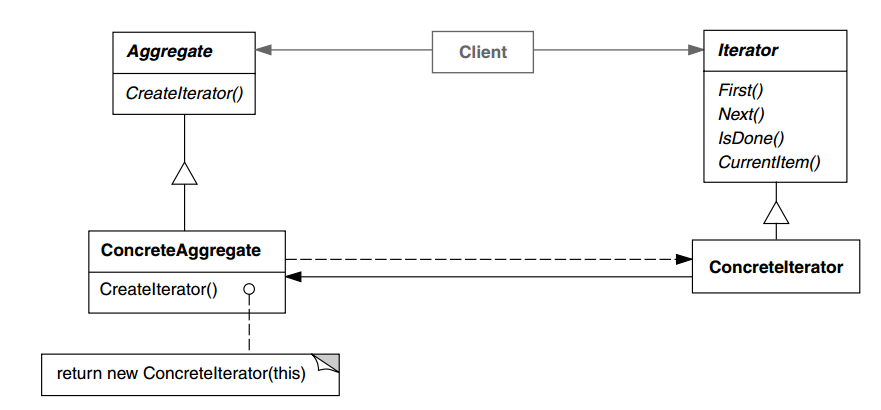
\includegraphics[scale=0.5]{5_padroes-contexto-funcional/5.3_comportamentais/5.3.04_iterator/diagram.png}
	\end{center}
\end{figure}

Exemplo Orientado a Objetos:

\begin{lstlisting}[caption={Iterator Orientação a Objetos},label=ooiterator]


    
\end{lstlisting}

Contexto Funcional:


\begin{lstlisting}[caption={Iterator Funcional},label=fpiterator]
    

    
\end{lstlisting}
\section{Mediator}


Nesse padrão, um objeto chamado de \textit{Mediator} age como intermediário 
entre um grupo de objetos, ficando responsável por qualquer 
interação entre eles. O \textit{Mediator} conhece todos 
esses objetos enquanto cada objeto conhece apenas o 
\textit{Mediator}, o que os torna 
mais independentes, simplificando sua reutilização
 e concentrando as dependências entre eles 
em um só lugar. \cite{gamma:1995}

A estrutura do padrão é apresentada na Figura \ref{mediator_struct}. 
Uma interface \texttt{Mediator} define as operações que um tipo de 
objeto \textit{Mediator} deve possuir. \texttt{ConcreteMediator} representa 
uma classe que implementa essas operações. Um \texttt{Colleague} 
é um objeto conhecido pelo \texttt{Mediator} e cada \texttt{ConcreteColleague} 
pode ser tanto um objeto que possui operações refletidas 
em outros objetos quanto ser um dos objetos afetados 
indiretamente por outro \texttt{Colleague}.

\begin{figure}[htb]
	\caption{\label{mediator_struct}Estrutura do \textit{Mediator}.}
	\begin{center}
	    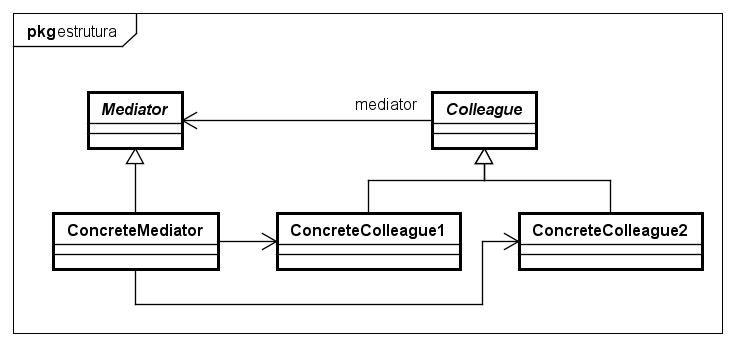
\includegraphics[scale=0.5]{5_padroes-contexto-funcional/5.3_comportamentais/5.3.05_mediator/mediator_estrutura.png}
	\end{center}
  \caption*{Fonte: O Autor (2021)}
\end{figure}

\subsection*{Exemplo Orientado a Objetos}

Como exemplo, é considerada uma janela de uma aplicação 
que apresenta diversos \textit{widgets}, entre eles uma caixa 
de entrada de texto e uma lista de seleção. Quando um item é 
selecionado na lista, o texto contido nele deve aparecer 
na caixa de entrada de texto. O \textit{Mediator} é responsável 
por alterar a caixa de entrada de texto quando um item 
é selecionado na lista, enquanto a lista é responsável 
por informar ao \textit{Mediator} quando um item for selecionado. 
A Figura \ref{mediator_exemplo} apresenta o diagrama 
de classes para esse exemplo. O Código \ref{oomediator} 
apresenta a implementação do padrão para esse exemplo.

\begin{lstlisting}[caption={\textit{Mediator} Orientado a Objetos.},label=oomediator]

abstract class DialogDirector {

  def ShowDialog() : Unit = {
    //Exibe o dialog
  }

  def CreateWidget()
  def WidgetChanged(widget: Widget)
}

class FontDialogDirector() extends DialogDirector {

  private var list : ListBox = null
  private var field : EntryField = null

  override def CreateWidget(): Unit = {
    this.list = new ListBox(this)
    this.field = new EntryField(this)
  }

  override def WidgetChanged(widget: Widget): Unit = {
    this.field.text = this.list.selection
  }
}

abstract class Widget(val director : DialogDirector) {
  def Changed() : Unit = director.WidgetChanged(this)
}

class EntryField(director : DialogDirector) extends Widget(director) {
  var text : String = ""
}

class ListBox(director : DialogDirector) extends Widget(director){
  private var _selection : String = ""
  def selection : String = _selection

  def SetSelection(selection : String) : Unit = {
    this._selection = selection
    Changed()
  }
}
    
\end{lstlisting}
\legend{Fonte: O Autor (2021)}

\begin{figure}[htb]
	\caption{\label{mediator_exemplo}Exemplo de \textit{Mediator}.}
	\begin{center}
	    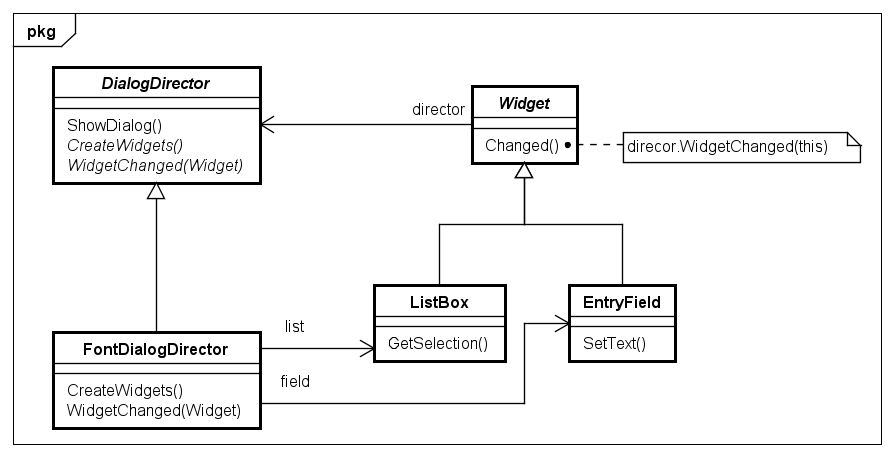
\includegraphics[scale=0.5]{5_padroes-contexto-funcional/5.3_comportamentais/5.3.05_mediator/mediator_exemplo.png}
	\end{center}
  \caption*{Fonte: O Autor (2021)}
\end{figure}

\subsection*{Contexto Funcional}

O Código \ref{fpmediator} demonstra a implementação 
funcional do \textit{Mediator}. Uma função é responsável por 
gerenciar as interdependências entre os valores 
dos tipos \texttt{EntryField}, definido na linha 2, e \texttt{ListBox}, 
definido na linha 12. Quando a função mediadora \texttt{ChangeSelection}, 
definida na linha 22, é chamada, ela precisa receber 
como parâmetro o elemento alvo e o elemento dependente, 
além das informações necessárias para executar a 
operação \texttt{ChangeListBoxSelection}. A função retorna 
tanto o \textit{colleague} alvo da operação 
quanto os \textit{colleagues} afetados, mantendo 
a função cliente que chama essa operação atualizada 
quanto ao estado de ambos os valores. 

A vantagem dessa abordagem é que ela torna possível 
que as funções dos \textit{colleagues} (no Código 
\ref{fpmediator}, \texttt{ChangeEntryFieldText} e 
\texttt{ChangeListBoxSelection}) sejam idependentes dos 
mediadodores, favorecendo seu reuso. A desvantagem 
é que é necessário realizar, na função cliente, 
um gerenciamento quanto ao estado de todos os 
\textit{colleagues}, já que a função mediadora 
deve ser pura e não realiza efeitos colaterais.

\begin{lstlisting}[caption={\textit{Mediator} Funcional.},label=fpmediator]
    
type EntryField = String

def ChangeEntryFieldText(text : String,
						 entryField: EntryField)
: EntryField =
  text
  
def GetText(entryField : EntryField) : String =
  entryField
  
type ListBox = String
  
def ChangeListBoxSelection(selection : String,
						   listBox: ListBox)
: ListBox =
  selection
  
def GetSelection(listBox : ListBox)  : String=
  listBox
  
def ChangeSelection(selection : String,
					entryField: EntryField,
					listBox : ListBox) : (EntryField, ListBox) = {
  (ChangeListBoxSelection(selection, listBox), ChangeEntryFieldText(selection, entryField))
}
	    
\end{lstlisting}
\legend{Fonte: O Autor (2021)}
\section{Memento}

O Memento permite armazenar e restaurar o estado interno de um 
objeto sem expor esse estado. Dessa forma, o encapsulamento do 
objeto em questão não é violado, mesmo seu estado sendo armazenado 
externamente.

Isso é alcançado através de uma classe Memento que armazena os 
atributos da classe que precisa ser salva (Originator). A geração 
de um objeto Memento só é possível através do próprio Originator, 
assim como a recuperação de seus atributos. Uma classe Caretaker 
é usada para armazenar objetos do tipo Memento e repassá-los para 
um Originator que precisa acessar o estado do Memento.

\begin{figure}[htb]
	\caption{\label{memento_struct}Estrutura do Memento}
	\begin{center}
	    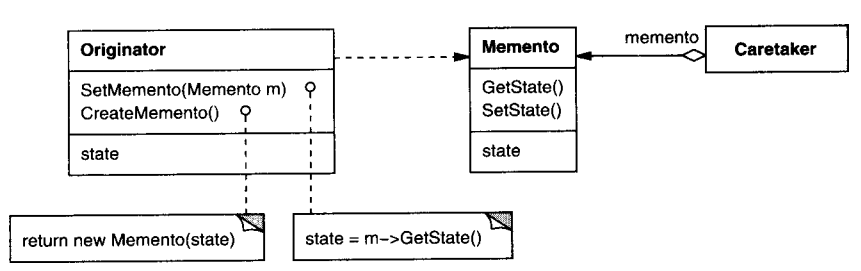
\includegraphics[scale=0.5]{5_padroes-contexto-funcional/5.3_comportamentais/5.3.06_memento/diagram.png}
	\end{center}
\end{figure}

Exemplo Orientado a Objetos:

\begin{lstlisting}[caption={Memento Orientação a Objetos},label=oomemento]



\end{lstlisting}

Contexto Funcional:

A ideia de armazenar estados anteriores pode ser alcançada com uma 
estrutura que armazena o valor atual do Originator e uma cópia do 
elemento desejado (ou uma lista armazenando um histórico de cópias). 
A partir dessa estrutura, é simples implementar funções que criam 
a cópia, atualizam o valor do Originator externamente e atualizam 
o valor do Originator a partir dos Mementos.

\begin{lstlisting}[caption={Memento Funcional},label=fpmemento]



\end{lstlisting}
\section{Observer}

O padrão Observer permite criar uma dependência de muitos 
objetos para um entre objetos. Dessa forma, quando um 
objeto em específico é alterado, um grupo de objetos 
pré-configurados é notificado. Esse comportamento é 
semelhante a um \textit{publish and subscribe}, onde 
um objeto é um \textit{publisher} que publica notificações 
para os objetos inscritos. A dinâmica do padrão pode ser 
vista no diagrama da figura \ref{observer_struct}.

\begin{figure}[htb]
	\caption{\label{observer_struct}Estrutura do Observer}
	\begin{center}
	    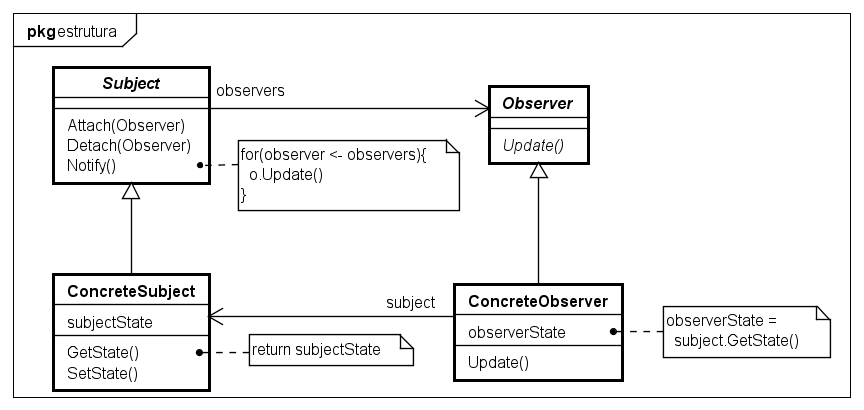
\includegraphics[scale=0.5]{5_padroes-contexto-funcional/5.3_comportamentais/5.3.07_observer/observer_estrutura.png}
	\end{center}
\end{figure}

\subsection*{Exemplo Orientado a Objetos}

Como exemplo, pode ser considerada uma aplicação 
gráfica que possui uma tabela e um gráfico de 
barras que apresentam informações de grupos 
A, B e C. Essas informações são dados utilizados 
pela aplicação que podem ser alterados por outros 
elementos gráficos, como botões ou caixas de texto. 
Para que a tabela e o gráfico estejam atualizados, 
eles são armazenados pela classe que centraliza 
esses dados de forma que ela os notifique 
caso os dados sejam atualizados. O diagrama 
de classes para o exemplo pode ser visto na figura 
\ref{observer_exemplo}, enquanto a implementação 
pode ser vista no código \ref{ooobserver}.

\begin{figure}[htb]
	\caption{\label{observer_exemplo}Exemplo de Observer}
	\begin{center}
	    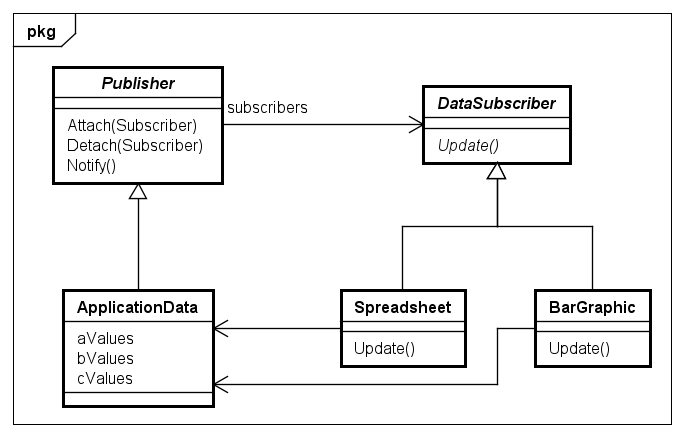
\includegraphics[scale=0.5]{5_padroes-contexto-funcional/5.3_comportamentais/5.3.07_observer/observer_exemplo.png}
	\end{center}
\end{figure}

\begin{lstlisting}[caption={Observer Orientação a Objetos},label=ooobserver]

abstract class Publisher {
  private var subscribers : List[DataSubscriber] = List.empty

  def Attach(subscriber: DataSubscriber) : Unit = {
    subscribers = subscriber :: subscribers
  }

  def Detach(subscriber: DataSubscriber) : Unit = {
    subscribers = subscribers.filter(sub => sub != subscriber)
  }

  def Notify() : Unit = {
    for(subscriber <- subscribers){
      subscriber.Update()
    }
  }
}

class ApplicationData extends Publisher {
  private var aValues : List[Int] = List.empty
  private var bValues : List[Int] = List.empty
  private var cValues : List[Int] = List.empty

  def SetValues(_aValues : List[Int],
                _bValues : List[Int],
                _cValues : List[Int]): Unit = {
    this.aValues = _aValues
    this.bValues = _bValues
    this.cValues = _cValues
    Notify()
  }

  def GetAValues() : List[Int] = aValues
  def GetBValues() : List[Int] = bValues
  def GetCValues() : List[Int] = cValues
}

trait DataSubscriber {
  def Update()
}

class Spreadsheet(val data : ApplicationData) extends DataSubscriber {
  override def Update(): Unit = {
    var aValues = data.GetAValues()
    var bValues = data.GetBValues()
    var cValues = data.GetCValues()
    //Atualiza a tabela com os novos valores
  }
}

class BarGraphic(data: ApplicationData) extends DataSubscriber {
  override def Update(): Unit = {
    var aBar = data.GetAValues().sum
    var bBar = data.GetBValues().sum
    var cBar = data.GetCValues().sum
    //Atualiza o gráfico com os novos valores
  }
}
    
\end{lstlisting}

\subsection*{Contexto Funcional}

O padrão Observer depende bastante de 
efeitos colaterais em sua implementação, 
já que depende de outros objetos serem avisados 
quando o estado do objeto observado for 
atualizado. Uma abordagem semelhante à vista 
no padrão Mediator, onde as funções clientes 
gerenciam os observáveis e os subordinados, 
poderia ser utilizada para trazer um resultado 
semelhante. Porém, existe uma abordagem - a 
programação reativa funcional - que se encaixa 
no contexto funcional e serve como alternativa 
para o padrão Observer\cite{reactiveprog}.

Programação reativa funcional pode ser entendida 
como a interseção entre programação reativa e 
programação funcional. Programação reativa traz a 
ideia de reagir ou responder a eventos, que são 
mensagens propagadas por um programa. Dessa forma, 
programação reativa funcional é um método de 
programação reativa que busca aproveitar os 
conceitos de composicionalidade e funções puras 
da programação funcional.\cite{reactiveprog}
\footnote{A linguagem Scala suporta programação 
reativa funcional através do \textit{framework} 
Akka, disponível em \url{https://akka.io/}.}
\section{State}

O State permite alterar o comportamento de um objeto baseado 
em seu estado interno. Uma interface define os comportamentos 
que dependem do estado do objeto e classes que a implementam 
definem a implementação dos mesmos. Dessa forma, o objeto 
principal delega as operações às classes que representam 
seu estado.

Esse padrão contribui para o reuso de operações comuns quando 
diversas classes relacionadas teriam que ser reinstanciadas 
durante uma mudança de estado. Também é permitido que o 
estado mude dinamicamente durante a execução.

\begin{figure}[htb]
	\caption{\label{state_struct}Estrutura do State}
	\begin{center}
	    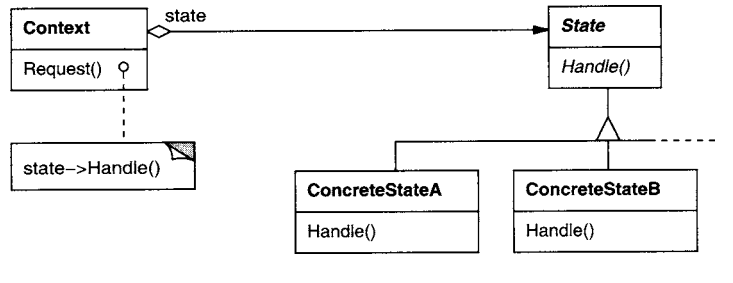
\includegraphics[scale=0.5]{5_padroes-contexto-funcional/5.3_comportamentais/5.3.08_state/diagram.png}
	\end{center}
\end{figure}

\subsection*{Exemplo Orientado a Objetos}

\begin{figure}[htb]
	\caption{\label{state_exemplo}Exemplo de State}
	\begin{center}
	    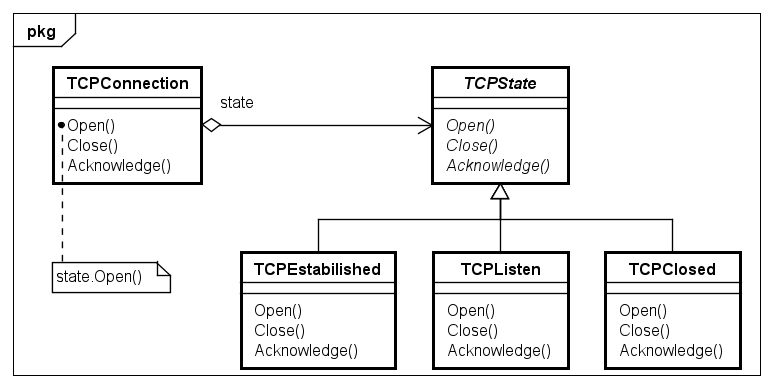
\includegraphics[scale=0.5]{5_padroes-contexto-funcional/5.3_comportamentais/5.3.08_state/state_exemplo.png}
	\end{center}
\end{figure}

\begin{lstlisting}[caption={State Orientação a Objetos},label=oostate]

trait State{
    def pressButton() : State
}

class OnState() extends State {
    def pressButton() : State = new OffState()
}

class OffState() extends State {
    def pressButton() : State = new OnState()
}

class Lamp(state : State) {
    def pressButton() : Unit {
        this.state = state.pressButton()
    }
}
    
\end{lstlisting}

\subsection*{Contexto Funcional}

\begin{comment}
Normalmente, a primeira alternativa que se tem em mente é 
o monad State. Porém, esse monad é focado em comportamentos 
que alteram o estado atual do nosso valor. Por mais que isso 
seja possível através do padrão State, por definição, sua 
intenção é fornecer comportamentos que não necessariamente 
altera o estado interno do valor.

Dessa forma, uma maneira interessante de definir o State 
no contexto funcional é utilizando uma case class que armazena, 
além dos valores comuns, um valor referente a um State. 
Esse State nada mais é do que outra clase class que 
irá armazenar, através de funções, os comportamentos que 
dependem de um estado. Da mesma forma que uma interface 
define as assinaturas das operações no exemplo orientado a 
objetos, aqui a definição da case class definirá que tipos 
de comportamentos a case class principal deverá possuir.

\begin{lstlisting}[caption={State Funcional},label=fpstate]
    
case class LampState(pressButton : () => Lamp)

case class Lamp(state : LampState)

def pressButton(lamp : Lamp) : Lamp =
    lamp.state.pressButton()

val onState : LampState = LampState(() => offState)

val offState : LampState = LampState(() => onState)
    
\end{lstlisting}

É importante notar que, aqui, quando o estado do valor 
principal precisa ser supostamente modificado, o que na 
verdade acontecerá é que a função da case class State 
irá retornar o nosso valor atualizado.

\end{comment}
\subsection{Strategy}

O padrão Strategy define grupos de algoritmos encapsulados e
 intercambiáveis para um determinado contexto. Esses 
 algoritmos podem ser definidos ou trocados em tempo de 
 execução, permitindo que os clientes que os utilizem possam
  alternar entre as implementações definidas livremente.

O Strategy soluciona o problema de classes relacionadas 
diferirem apenas em algum comportamento, permitindo que 
esse comportamento possa ser isolado e o resto da implementação 
das classes reaproveitado. Ele também evita a utilização de 
muitas operações condicionais. Ao invés de verificar qual 
deve ser o comportamento toda vez que ele precisar ser 
executado, o comportamento é pré-definido pelo contexto.

\begin{figure}[htb]
	\caption{\label{fig_grafico}Estrutura do Strategy}
	\begin{center}
	    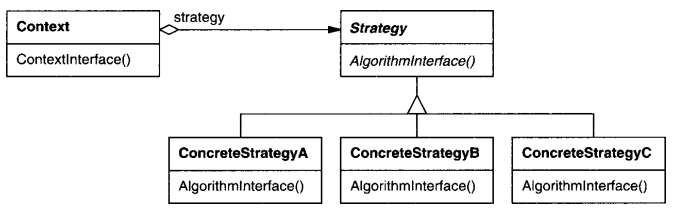
\includegraphics[scale=0.5]{5_padroes-contexto-funcional/5.3_comportamentais/5.3.09_strategy/diagram.png}
	\end{center}
\end{figure}

Exemplo Orientado a Objetos:

\begin{lstlisting}[caption={Strategy Orientação a Objetos},label=oostrategy]
    
    trait Strategy {
        def execute(a : Int, b : Int) : Int
    }

    class ConcreteStrategyAdd() extends Strategy {
        def execute(a : Int, b : Int) : Int = {
            a + b
        }
    }

    class ConcreteStrategySubtract() extends Strategy {
        def execute(a : Int, b : Int) : Int = {
            a - b
        }
    }

    class ConcreteStrategyMultiply() extends Strategy {
        def execute(a : Int, b : Int) : Int = {
            a * b
        }
    }

    class Context() {
        
        private var strategy : Strategy

        def setStrategy(strategy : Strategy) =
            this.strategy = strategy

        def executeStrategy(a : Int, b : Int) : Int =
            this.strategy.execute(a, b)

    }

\end{lstlisting}

Contexto Funcional:

No contexto funcional, o encapsulamento de algoritmos 
ou de comportamentos diferentes pode ser alcançado através 
de funções de alta ordem (high-order functions). Nesse caso,
 não é necessário definir interfaces ou objetos para encapsular 
 esses comportamentos, eles podem ser recebidos através da 
 passagem de parâmetro como funções:


\begin{lstlisting}[caption={Strategy Funcional},label=fpstrategy]
    
    def executeAdd(a : Int, b: Int) : Int = {
        a + b
    }

    def executeSubtract(a : Int, b: Int) : Int = {
        a - b
    }

    def executeMultiply(a : Int, b: Int) : Int = {
        a * b
    }

    def executeStrategy(execute : (a : Int, b : Int) => Int) : Int =
        execute(a, b)

\end{lstlisting}

Porém, existe uma desvantagem. A função [executeStrategy] 
acima aceita qualquer função que receba dois parâmetros 
inteiros e retorne um valor inteiro. Isso significa que 
qualquer função definida que não faça parte da solução 
mas que atenda a esse requisito pode ser usada como uma
 estratégia:

 \begin{lstlisting}[caption={Strategy Funcional: Problema},label=fpstrategyproblem]
    
    def executeOutOfScope(a : Int, b : Int) : Int = {
        a ** 2 + b ** 2
    }

\end{lstlisting}

No caso orientado a objetos, os comportamentos estão 
ecanpsulados em interfaces, o que torna mais segura a 
implementação dos comportamentos.
\section{Template Method}

A ideia do Template Method é fornecer um esqueleto para um algoritmo 
e deixar para outras classes a tarefa de implementar as funções que 
compõem esse algoritmo. Uma classe abstrata define a operação Template 
Method, onde são executas as etapas do algoritmo, definidas em função 
das operações abstratas ainda não implementadas.

Esse padrão ajuda a evitar repetição de código, concentrando 
em apenas uma classe a estrutura de uma operação. Além disso, 
não só apenas a estrutura do algoritmo como qualquer etapa em 
comum para todas as subclasses pode ser concentrada na superclasse, 
evitando mais ainda a repetição do código. A estrutura do padrão 
pode ser vista na figura \ref{tpmethod_struct}.

\begin{figure}[htb]
	\caption{\label{tpmethod_struct}Estrutura do Template Method}
	\begin{center}
	    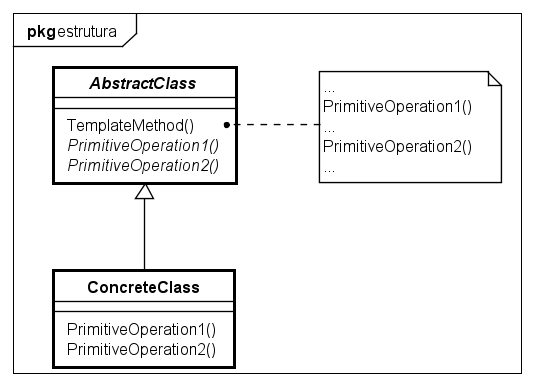
\includegraphics[scale=0.5]{5_padroes-contexto-funcional/5.3_comportamentais/5.3.10_template-method/templatemethod_estrutura.png}
	\end{center}
\end{figure}

\subsection*{Exemplo Orientado a Objetos}

Como exemplo pode ser consideraro um \textit{framework} que fornece uma classe para abrir documentos. Essa classe possui operações abstratas para cada etapada da abertura de um documento, de forma que as subclasses que a estendem podem definir formas diferentes de abrir documentos de tipos diferentes. A operação AddDocument é o template method, responsável por chamar as demais operações implementadas pelas subclasses. 
O diagrama de classes do exemplo pode ser visto na imagem \ref{tpmethod_exemplo}, 
enquanto a implementação pode ser vista no código \ref{ootpmethod}.

\begin{figure}[htb]
	\caption{\label{tpmethod_exemplo}Exemplo de Template Method}
	\begin{center}
	    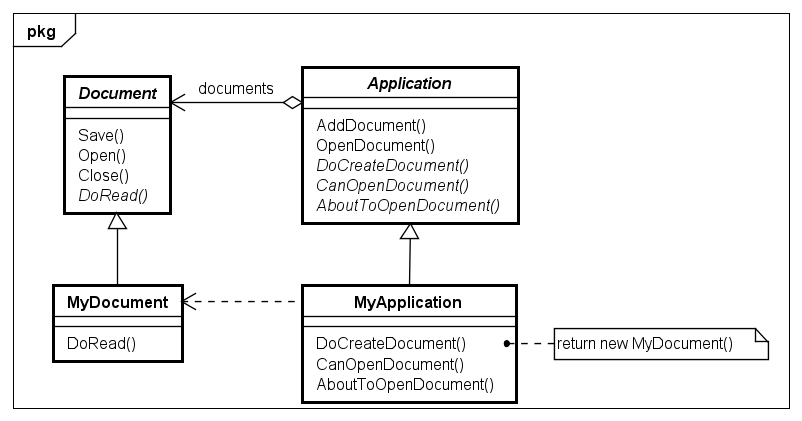
\includegraphics[scale=0.5]{5_padroes-contexto-funcional/5.3_comportamentais/5.3.10_template-method/templatemethod_exemplo.png}
	\end{center}
\end{figure}

\begin{lstlisting}[caption={Template Method Orientação a Objetos},label=ootpmethod]

abstract class Document {
  def Save() : Unit = {
    //Salva um document
  }
  def Open() : Unit = {
    //Abre um documento
  }
  def Close() : Unit = {
    //Fecha um documento
  }
  def DoRead()
}

class MyDocument extends Document {
  def DoRead(): Unit = {
    //Faz leitura do documento
  }
}

abstract class Application {

  var documents : List[Document] = List.empty

  def AddDocument(document : Document) : Unit = {
    documents = document :: documents
  }

  def OpenDocument(fileName : String) : Unit = {
    if(!CanOpenDocument(fileName)){

    } else {
      val doc = DoCreateDocument()
      AddDocument(doc)
      AboutToOpenDocument(doc)
      doc.Open()
      doc.DoRead()
    }
  }

  def DoCreateDocument() : Document
  def CanOpenDocument(fileName : String) : Boolean
  def AboutToOpenDocument(document : Document)
}

class MyApplication extends Application {
  def DoCreateDocument() : Document = new MyDocument
  def CanOpenDocument(fileName : String) : Boolean = {
    //Verifica se documento pode ser aberto
    true
  }
  def AboutToOpenDocument(document : Document): Unit = {
    //Operação ao abrir documento
  }
}

\end{lstlisting}

\subsection*{Contexto Funcional}

No contexto funcional, a mesma ideia pode ser alcançada 
através de funções de alta ordem e composição de funções. 
O método OpenDocument (o \textit{template method}) é 
uma função de alta ordem que recebe como parâmetro todas 
as funções necessárias para executar o algoritmo. 
O exemplo pode ser visto no código \ref{fptpmethod}.

\begin{lstlisting}[caption={Template Method Funcional},label=fptpmethod]
    
object Application {

  trait Document {
    def Open()
    def DoRead()
  }

  def AddDocument(document : Document,
                  documents : List[Document]) : List[Document] =
    document :: documents


  def OpenDocument(filename : String,
                   documents : List[Document],
                   DoCreateDocument : () => Document,
                   CanOpenDocument : (String) => Boolean,
                   AboutToOpenDocument : (Document) => Unit) : Unit = {
    if(!CanOpenDocument(filename)){
      //...
    } else {
      var _documents : List[Document] = Nil
      val doc = DoCreateDocument()
      _documents = AddDocument(doc, documents)
      AboutToOpenDocument(doc)
      doc.Open()
      doc.DoRead()
    }
  }

}

\end{lstlisting}

Para definir uma implementação do algoritmo, basta 
definir uma nova função que é a combinação do método 
template com as funções que representam as etapas do 
algoritmo. O código \ref{algotpmethod} define uma 
nova função, MyApplicationOpenDocument, que recebe 
como parâmetro o nome do arquivo e uma lista de 
documentos. Ela retorna a função OpenDocument com as 
funções específicas para o tipo de documento 
desejado sendo passadas como parâmetro, nas linhas 
6, 7 e 8. Dessa forma, a função MyApplicationOpenDocument 
pode ser reutilizada da mesma forma que a classe 
MyApplication seria reutilizada no exemplo orientado 
a objetos.

\begin{lstlisting}[caption={Definição do algoritmo},label=algotpmethod]
    
val MyApplicationOpenDocument = 
    (filename : String, documents : List[Document]) => 
      OpenDocument(filename, documents,
        CreateMyDocument,
        MyCanOpenDocument,
        MyAboutToOpenDocument)

\end{lstlisting}

\begin{comment}
\subsection*{Vantagens e Desvantagens}

É possível definir novos \textit{templates} com operações 
pré-definidas facilmente criando uma combinação parcial 
das funções necessárias para a execução do algoritmo. 
Assim, poderia ser implementada uma função cujas 
operações DoCreateDocument e CanOpenDocument sejam idênticas, 
mas que permitisse implementações diferentes de 
AboutToOpenDocument. Para que isso pudesse ser feito 
no exemplo orientado a objetos, seria necessário 
definir uma nova subclasse abstrata de Application.
\end{comment}

\section{Visitor}

O padrão Visitor permite realizar 
operações em uma estrutura de objetos sem precisar alterá-los 
e sem precisar que os objetos conheçam as 
operações que estão sendo realizadas. \cite{gamma:1995}

Uma estrutura alvo de um Visitor pode possuir objetos de 
classes diferentes. Por isso, o padrão deve implementar 
uma operação Visit para cada uma dessas classes, 
através de uma sobrecarga de métodos. Para que essa 
abordagem funcione, as classes da estrutura devem implementar 
uma operação Accept que recebe como parâmetro um 
Visitor genérico e chama sua operação Visit, 
passando uma referência para a instância atual 
(através da palavra chave this) 
como parâmetro. Dessa forma, a função chamada é a 
que recebe como parâmetro uma instância da 
classe em questão.

Esse padrão permite estender objetos para novas operações 
sem comprometer sua implementação ou poluir as classes com 
diversas operações que não são de sua responsabilidade. 
Sua estrutura pode ser vista na Figura \ref{visitor_struct}.

\begin{figure}[htb]
	\caption{\label{visitor_struct}Estrutura do Visitor}
	\begin{center}
	    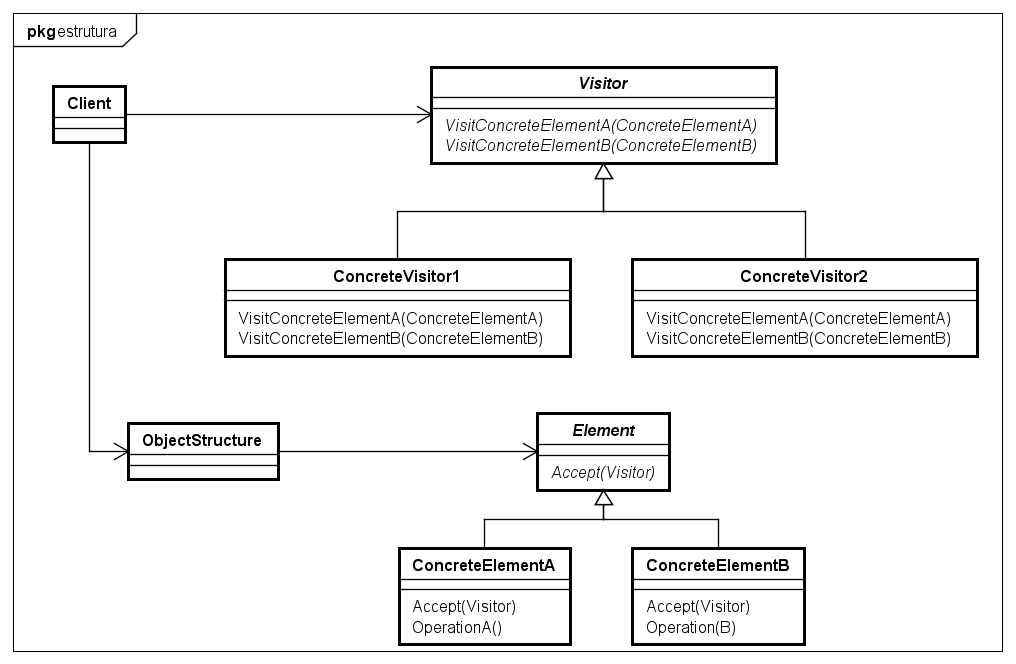
\includegraphics[scale=0.5]{5_padroes-contexto-funcional/5.3_comportamentais/5.3.11_visitor/visitor_estrutura.png}
	\end{center}
\end{figure}

\subsection*{Exemplo Orientado a Objetos}

Um compilador precisa fazer a análise de árvore abstrata sintática de 
um programa. Essa análise inclui diversas operações diferentes, como 
checagem de tipos e geração de código. Para que os nós da árvore 
não precisem implementar essas operações, elas implementam uma operação 
genérica que recebe como parâmetro qualquer Visitor. Dessa forma, para 
cada operação desejada, basta implementar uma nova classe Visitor 
que percorrerá os elementos da árvore abstrata sintática. O diagrama 
de classes para o exemplo pode ser visto na Figura \ref{visitor_exemplo1}, 
enquanto a implementação pode ser vista no Código \ref{oovisitor}.

\begin{figure}[htb]
	\caption{\label{visitor_exemplo1}Exemplo de Visitor}
	\begin{center}
	    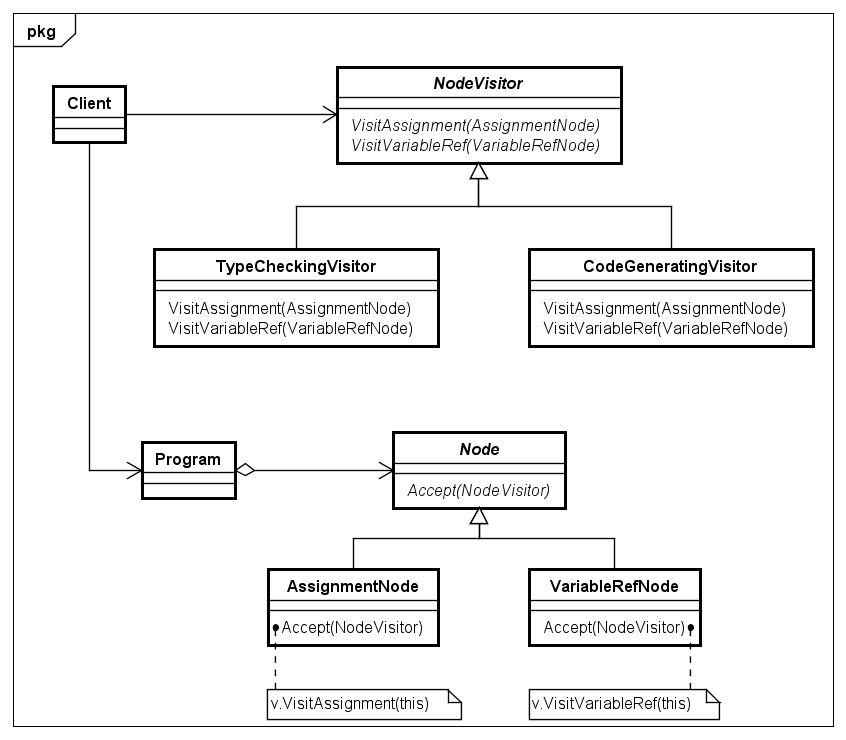
\includegraphics[scale=0.5]{5_padroes-contexto-funcional/5.3_comportamentais/5.3.11_visitor/visitor_exemplo.png}
	\end{center}
\end{figure}

\begin{lstlisting}[caption={Visitor Orientação a Objetos},label=oovisitor]

trait NodeVisitor {
  def VisitAssignment(node : AssignmentNode)
  def VisitVariableRef(node : VariableRefNode)
}

trait Node {
  def Accept(visitor : NodeVisitor)
}

class AssignmentNode extends Node {
  def Accept(visitor: NodeVisitor): Unit = visitor.VisitAssignment(this)
}

class VariableRefNode extends Node {
  def Accept(visitor : NodeVisitor) : Unit = visitor.VisitVariableRef(this)
}

class TypeCheckingVisitor extends NodeVisitor {

  def VisitAssignment(node: AssignmentNode): Unit = {
    //Operações de checagem de tipo para atribuição
  }

  def VisitVariableRef(node: VariableRefNode): Unit = {
    //Operações de checagem de tipo para variáveis
  }
}

class CodeGeneratingVisitor extends NodeVisitor {

  def VisitAssignment(node: AssignmentNode): Unit = {
    //Operações de geração de código para atribuição
  }

  def VisitVariableRef(node: VariableRefNode): Unit = {
    //Operações de geração de código para variáveis
  }
}

\end{lstlisting}

\subsection*{Contexto Funcional}

Uma das maiores vantagens do padrão Visitor 
é o uso de multimétodos, onde um método é 
executado de forma dinâmica, baseado no tipo 
de um objeto em tempo de execução. Essa 
funcionalidade é possível através do polimorfismo 
nas linguagens orientadas a objetos.\cite{gamma:1995}

Uma funcionalidade semelhante que algumas 
linguagens funcionais implementam é o 
\textit{pattern matching}\cite{realworldhaskell,
functionalscala}. 
Ela consiste em avaliar um valor a partir de 
um padrão predefinido, ou seja, a operação 
que será realizada dependerá do valor avaliado
\cite{functionalscala}. 
No caso do padrão Visitor, todos os métodos 
sobrecarregados que executam a operação 
em cada tipo de elemento da coleção são 
substituídos por um único método que 
reconhece o tipo de valor da estrutura. 
Essa abordagem possui suas desvantagens, 
dependendo de como a linguagem implementa 
o \textit{pattern matching}. No caso de Scala, 
pode ser necessário incluir nos valores da 
estrutura um valor enumerável que identifica o 
tipo do elemento. 

O Código \ref{fpvisitor} demonstra como o 
exemplo orientado a objetos pode ser implementado. 
O tipo Node, definido na linha 2, armazena um valor 
enumerável com os tipos de nó suportados 
pela aplicação, além dos outros valores 
armazenados por um nó - representados pelo tipo 
NodeValue. A função DefineNodeVisitor, definida 
na linha 4, aproveita o uso de funções de alta ordem 
para gerar tipos diferentes de Visitor. Ela 
recebe como parâmetro duas funções, uma que 
realiza uma operação para o tipo de nó Assignment e 
outra que realiza uma operação para o tipo de 
nó VariableRef. Ela retorna uma nova função - o 
Visitor - que recebe como parâmetro uma coleção 
de nós e retorna a mesma coleção após aplicadas 
todas as operações. Nas linhas 9 e 11 é onde 
ocorre o \textit{pattern matching}. Uma operação 
de desconstrução é aplicada na tupla que representa 
um nó. Caso o nó seja do tipo Assignment, o 
primeiro caso é executado. Caso seja do tipo 
VariableRef, o segundo caso é executado.

\begin{lstlisting}[caption={Visitor Funcional},label=fpvisitor]
    
type Node = (NodeType.Value, NodeValue)

def DefineNodeVisitor(AssignmentNodeVisitor : NodeValue => Node,
                      VariableRefNodeVisitor : NodeValue => Node) :
List[Node] => List[Node] = {
  (nodes : List[Node]) => {
    nodes.map {
      case (NodeType.AssignmentNode, value) => 
        AssignmentNodeVisitor(value)
      case (NodeType.VariableRefNode, value) => 
        VariableRefNodeVisitor(value)
    }
  }
}
    
\end{lstlisting}

% ----------------------------------------------------------
% PARTE
% ----------------------------------------------------------
%\part{Resultados}
% ----------------------------------------------------------
\part{Resultados}

% ---
% Apresentação dos Resultados
% ---
\chapter{Apresentação dos Resultados}
% ---

Nos capítulos anteriores, foram analisados todos 
vinte e três padrões de projeto \textit{Gang of 
Four}, com o objetivo de extrair o problema 
resolvido pelo padrão e analisar, a partir dos 
conceitos de programação funcional apresentados, 
como uma solução para o mesmo problema poderia ser 
alcançada. 

Foi possível separar as análises realizadas em 
quatro grandes grupos, com o primeiro sendo 
dividido em três subgrupos: 

\begin{alineas}
    \item Padrões resolvidos por funções de alta ordem
    \begin{alineas}
        \item Funções de alta ordem como alternativa a classes abstratas ou interfaces
        \item Valores que armazenam funções
        \item Funções que armazenam valores em closures
    \end{alineas}
    \item Padrões com soluções alternativas
    \item Padrões sem diferenças relevantes
    \item Padrões que não fazem sentido no contexto funcional
\end{alineas}

Esses grupos estão organizados na tabela 
\ref{resultados}, onde são apresentados os 
padrões pertencentes a cada grupo com a 
quantidade de padrões pertencentes ao grupo. 
Cada grupo será explicado com mais detalhes 
no decorrer do capítulo.

\begin{quadro}[htb]
    \caption{\label{resultados}Agrupamento de análises dos padrões}
    \begin{tabular}{@{}llll@{}}
        \toprule
                                  &                            & Padrões                 & Quantidade         \\ \midrule
        \multirow{14}{*}{Grupo A} & \multirow{7}{*}{A.1} & Factory Method          & \multirow{7}{*}{7} \\
                                  &                            & Builder                 &                    \\
                                  &                            & Adapter                 &                    \\
                                  &                            & Bridge                  &                    \\
                                  &                            & Proxy                   &                    \\
                                  &                            & Strategy                &                    \\
                                  &                            & Template Method         &                    \\ \cmidrule(r){2-4}
                                  & \multirow{3}{*}{A.2} & Abstract Factory        & \multirow{3}{*}{3} \\
                                  &                            & Command                 &                    \\
                                  &                            & State                   &                    \\ \cmidrule(r){2-4}
                                  & \multirow{4}{*}{A.3} & Composite               & \multirow{4}{*}{4} \\
                                  &                            & Decorator               &                    \\
                                  &                            & Chain of Responsibility &                    \\
                                  &                            & Interpreter             &                    \\ \cmidrule(r){1-4}
        \multicolumn{2}{l}{\multirow{3}{*}{Grupo B}}           & Iterator                & \multirow{3}{*}{3} \\
        \multicolumn{2}{l}{}                                   & Observer                &                    \\
        \multicolumn{2}{l}{}                                   & Visitor                 &                    \\ \cmidrule(r){1-4}
        \multicolumn{2}{l}{\multirow{3}{*}{Grupo C}}           & Façade                  & \multirow{3}{*}{3} \\
        \multicolumn{2}{l}{}                                   & Flyweight               &                    \\
        \multicolumn{2}{l}{}                                   & Mediator                &                    \\ \cmidrule(r){1-4}
        \multicolumn{2}{l}{\multirow{3}{*}{Grupo D}}           & Prototype               & \multirow{3}{*}{3} \\ 
        \multicolumn{2}{l}{}                                   & Singleton               &                    \\
        \multicolumn{2}{l}{}                                   & Memento                 &                    \\ \cmidrule(r){1-4} %\cmidrule(l){4-4} 
    \end{tabular}
\end{quadro}

\section{Padrões resolvidos por funções de alta ordem}

Entre as soluções vistas, a que é aplicada na 
maior parte dos padrões é o uso de funções de alta 
ordem como alternativa a interfaces ou classes. 
Um total de catorze dos vinte e três padrões 
se encaixa nessa categoria. Por isso, ainda foi 
possível dividir esses padrões em três  
subcategorias quanto a como as funções de alta 
ordem foram aplicadas. Alguns padrões acabam se 
encaixando em mais de uma delas, mas para 
evitar repetições e para simplificar o agrupamento, 
cada padrão será explicado no grupo mais próximo 
da solução proposta. 

% Factory Method, Builder, Adapter, Bridge, 
% Proxy, Strategy, Template Method
\subsection{Funções de alta ordem como alternativa a 
            classes abstratas ou interfaces}

Como foi visto no mapeamento de conceitos orientados 
a objeto para conceitos de programação funcional, 
funções de alta ordem podem servir como alternativas 
para o uso de interfaces. Alguns dos padrões analisados 
baseiam-se no uso de interfaces para definir a assinatura 
de funções que a classe cliente deve receber. De forma 
equivalente, é possível que uma função cliente recebe, 
por parâmetro, uma função com a assinatura equivalente 
à da interface. Essa é a abordagem utilizada com os 
padrões Builder, Adapter, Bridge, Proxy e Strategy. 

De forma semelhante, as funções de alta ordem são 
alternativas ainda mais interessantes ao uso de 
classes abstratas, como é o caso dos padrões 
Factory Method e Template Method. Ambos baseiam-se 
em definir uma operação abstrata que deve ser 
implementada por uma subclasse. Uma alternativa 
a essa implementação é fazer com que as funções 
que dependam dessa operação abstrata a recebam 
por parâmetro.

% Abstract Factory, Command, State
\subsection{Valores que armazenam funções}

Os padrões Abstract Factory, Command e 
State também baseiam-se em passar funções de 
alta ordem como parâmetro para funções clientes. 
Porém, para esses três padrões existe uma quantidade 
maior de funções que o cliente deve receber. Além 
disso, pode ser mais interessante que as implementações 
dessas funções sejam dependentes entre si, ou seja, 
todas as funções de um Strategy pertençam a uma mesma 
estratégia, todas as funções do Abstract Factory criem 
o mesmo tipo de valor e a função de desfazer do 
Command esteja relacionada à função principal executada. 
Agrupar essas funções em um mesmo valor pode 
contribuir para retirar das funções clientes a 
responsabilidade de garantir que elas possuam 
essa equivalência.

% Composite, Decorator, Chain of Responsibility, Interpreter
\subsection{Funções que armazenam valores em closures}

Algumas implementações basearam-se em definir funções 
que retornam novas funções. Isso é necessário para 
que seja possível configurar as funções retornadas 
com valores recebidos por parâmetro pelas funções 
que as criam. Esse é o comportamento definido pelas 
closures, onde uma determinada função armazena 
um valor do escopo da função que a retornou. 

O padrão Composite define funções para gerar os 
elementos nós e os elementos folha. Dessa forma, 
a partir de uma única função, vários elementos 
folha e nó configurados com valores diferentes 
podem ser gerados.

De forma semelhante, o padrão Decorator define 
funções que podem receber como parâmetro valores 
variados enquanto retorna uma nova função com 
a mesma assinatura da função decorada. 

O padrão Chain of Responsibility aproveita a mesma 
ideia para gerar as funções da cadeia. O tópico e 
a próxima função da cadeia são passadas por parâmetro 
previamente, armazenadas na closure e reaproveitadas 
na função retornada. 

Por fim, o padrão Interpreter apresenta um comportamento 
semelhante ao Composite, definindo funções que retornam 
os elementos terminais e não terminais, permitindo 
inclusive definir funções mais genéricas que recebem 
a função que aplica a regra da gramática por parâmetro.

% Iterator, Observer, Visitor
\section{Padrões com soluções alternativas}

Os padrões Iterator, Observer e Visitor possuem 
implementações alternativas que não necessariamente 
seguem à risca a ideia do padrão. No caso do Iterator, 
existe a diferença entre o gerencimaneto por parte 
do cliente e por parte da coleção entre as 
alternativas orientada a objetos e funcional. No 
caso do Observer, o conceito no qual ele se 
baseia - programação reativa - é levado em 
consideração ao substituí-lo pela programação 
reativa funcional. Já o Visitor, apesar de também 
aproveitar-se de funções de alta ordem, na verdade 
é resolvido pelo recurso \textit{pattern matching}, 
que não é um conceito exclusivamente funcional, 
porém costuma ser implementado em linguagens 
funcionais. Nesse caso, o padrão não foi 
resolvido por programação funcional em si, 
mas sim por uma alternativa próxima. 

% Façade, Flyweight, Mediator
\section{Padrões sem diferenças relevantes}

Alguns dos padrões analisados possuem 
uma implementação muito semelhante ou 
equivalente entre os contextos orientados 
a objeto e funcionais, como se a solução 
proposta pelo padrão estivesse apenas 
sendo reutilizada por si só, sem 
recursos adicionais oriundos da programação 
funcional que contribuem para a 
resolução do problema. 

Da mesma forma que o padrão Façade orientado 
a objetos baseia-se no acesso entre as classes, 
a implementação funcional baseia-se no acesso 
entre módulos. Como ambas as ideias são 
análogas, a implementação do padrão na verdade 
não possui mudanças significativas. 

Da mesma forma, o padrão Flyweight, tanto no 
contexto orientado a objetos quanto no funcional, 
é implementado através de memoização. Já o Mediator 
baseia-se em possuir uma função (ou classe) que 
gerencia as dependências entre valores (ou objetos). 
No caso desses dois padrões, ambos possuem 
pequenas diferenças como consequência de suas 
implementações - por exemplo, não existem os dois 
tipos de Flyweight intrínseco ou extrínseco 
graças à imutabilidade e há a necessidade do 
cliente gerenciar a mudança de estado dos 
\textit{colleagues} no Mediator -, mas a ideia 
por trás da implementação de ambos é análoga 
à versão orientada a objetos.

% Prototype (imutabilidade), Singleton (funções puras), 
% Memento (imutabilidade)
\section{Padrões que não fazem sentido no contexto funcional}

Para alguns padrões, o problema proposto deixa 
de existir graças aos conceitos já implementados 
em linguagens funcionais. No caso dos padrões 
analisados neste trabalho, encaixam-se nessa 
categoria o Singleton, o Prototype e o Memento. 

Como a intenção do padrão Singleton pode 
ser entendida como a definição de uma variável 
global, sua implementação no contexto funcional 
viola o conceito de funções puras e imutabilidade - 
para o caso em que o Singleton armazena algum 
estado compartilhado. Portanto, tentar 
implementá-lo não faz sentido. 

Para o caso do Prototype, como visto anteriormente, 
o uso de estruturas de dados imutáveis trazem um 
gerenciamento mais simples de memória. Não existe 
preocupação quanto a uma referência compartilhada 
para um mesmo valor, já que seu estado não pode ser 
modificado. Dessa forma, não há a necessidade de 
definir uma implementação que compartilhe dados.

Por fim, o padrão Memento, também graças à 
imutabilidade, não precisaria se preocupar quanto 
a expor o estado interno de um valor. Assim, é 
possível gerar \textit{snapshots} apenas copiando 
valores anteriores, sem preocupações adicionais. 

%% ---
% Avaliação dos Resultados
% ---
\chapter{Avaliação dos Resultados}
% ---

% É importante descrever quais resultados são mais
% relevantes e como eles contribuem com a área 
% de estudo
%\section{Avaliação}



% Um bom embasamento teórico é fundamental para 
% dar credibilidade aos resultados da pesquisa 
% Portanto, o investigador deve comparar as 
% ideais de outros autores com a descoberta do 
% seu trabalho
%\section{Comparação com a literatura}



% Quando a coleta de dados é representativa, 
% o pesquisador pode fazer generalizações
%\section{Generalização}

% ---
% Conclusão
% ---
\chapter{Conclusão}
% ---

\lipsum[31-33]


% ----------------------------------------------------------
% Finaliza a parte no bookmark do PDF
% para que se inicie o bookmark na raiz
% e adiciona espaço de parte no Sumário
% ----------------------------------------------------------
\phantompart


% ----------------------------------------------------------
% ELEMENTOS PÓS-TEXTUAIS
% ----------------------------------------------------------
\postextual
% ----------------------------------------------------------

% ----------------------------------------------------------
% Referências bibliográficas
% ----------------------------------------------------------
\bibliography{functionaldesignpatterns-references}





%---------------------------------------------------------------------
% INDICE REMISSIVO
%---------------------------------------------------------------------
\phantompart
\printindex
%---------------------------------------------------------------------

\end{document}
